
% Diese Datei gilt als Master für die Latex-Kompilierung.
% Hier werden die einzelnen Unterdateien zusammengeführt.
% Im Latex-Programm daher immer diese Datei kompilieren und nicht die Unterdateien selbst!
% Wenn eine neue Datei hinzugefügt wurde, muss diese hier unbedingt eingebunden werden!!
% Gemeinsame Einstellungen aus der Präambel
% PRÄAMBEL für Latexdokumente
% Diese Datei muss als erstes in einem neuen Latexdokument eingebunden werden (per \insert )
% und darf NICHT (!) in einen document-Block eingebettet werden!

%\documentclass[fontsize=11pt, paper=a4, headinclude, twoside=false, parskip=half+, pagesize=auto, numbers=noenddot, open=right, toc=listof, toc=bibliography]{scrreprt}
\documentclass[headsepline,footsepline,footinclude=false,parskip=half+, oneside,fontsize=11pt,paper=a4,listof=totoc,bibliography=totoc]{scrbook} % one-sided

% PDF-Kompression
\pdfminorversion=5
\pdfobjcompresslevel=1

% Allgemeines
%\usepackage[automark]{scrpage2} % Kopf- und Fußzeilen
\usepackage{amsmath,marvosym} % Mathesachen
\usepackage[T1]{fontenc} % Ligaturen, richtige Umlaute im PDF
\usepackage[utf8]{inputenc}% UTF8-Kodierung für Umlaute usw

% Schriften
%\usepackage{mathpazo} % Palatino für Mathemodus
%\usepackage{mathpazo,tgpagella} % auch sehr schöne Schriften
% \usepackage{fourier}
\usepackage{setspace} % Zeilenabstand

% Schriften-Größen
\setkomafont{disposition}{\normalfont\bfseries} % use serif font for headings
\linespread{1.05} % adjust line spread for mathpazo font
%\setkomafont{chapter}{\Huge\rmfamily} % Überschrift der Ebene
%\setkomafont{section}{\Large\rmfamily}
%\setkomafont{subsection}{\large\rmfamily}
%\setkomafont{subsubsection}{\rmfamily}
%\setkomafont{chapterentry}{\large\rmfamily} % Überschrift der Ebene in Inhaltsverzeichnis
%\setkomafont{descriptionlabel}{\bfseries\rmfamily} % für description Umgebungen
%\setkomafont{captionlabel}{\small\bfseries}
%\setkomafont{caption}{\small}
%\usepackage{xspace} % Für manuelle Abstände

% Sprache: Deutsch
\usepackage[ngerman]{babel} % Silbentrennung
\usepackage[ngerman]{translator} % Deutsche Überschriften

% PDF
\usepackage[ngerman,pdfauthor={Joshua Hirsch},  pdfauthor={Joshua Hirsch}, pdftitle={Bachelorarbeit}, breaklinks=true,baseurl={http://www.corpuls.world}]{hyperref}
%\usepackage[final]{microtype} % mikrotypographische Optimierungen
\usepackage{url}
\usepackage{pdflscape} % einzelne Seiten drehen können

%  Bibliographie
\usepackage{bibgerm} % Umlaute in BibTeX
\usepackage{epigraph} % Hervorgehobene Zitate

% Glossar
\usepackage[acronym,nonumberlist,toc]{glossaries}
\renewcommand*{\glspostdescription}{} %Den Punkt am Ende jeder Beschreibung deaktivieren
\makeglossaries

% Tabellen
\usepackage{multirow} % Tabellen-Zellen über mehrere Zeilen
\usepackage{multicol} % mehre Spalten auf eine Seite
\usepackage{tabularx} % Für Tabellen mit vorgegeben Größen
\usepackage{longtable} % Tabellen über mehrere Seiten
\usepackage{array}
\usepackage{float}
\usepackage{rotating} % Tabellen im Querformat

% Bilder
\usepackage{graphicx} % Bilder
\usepackage{color} % Farben
\usepackage{floatflt} % Textumfluss
\usepackage{caption} % Verbesserte Untertitel
\graphicspath{{images/}}
\DeclareGraphicsExtensions{.pdf,.png,.jpg} % bevorzuge pdf-Dateien
\usepackage{subfigure} % mehrere Abbildungen nebeneinander/übereinander
\newcommand{\subfigureautorefname}{\figurename} % um \autoref auch für subfigures benutzen
\usepackage[all]{hypcap} % Beim Klicken auf Links zum Bild und nicht zu Caption gehen
\usepackage[section]{placeins} % Bilder nur in zugehöriger Section unterbringen

% Bildunterschrift
\setcapindent{0em} % kein Einrücken der Caption von Figures und Tabellen
\setcapwidth{0.9\textwidth}
\setlength{\abovecaptionskip}{0.2cm} % Abstand der zwischen Bild- und Bildunterschrift

% Quellcode
\usepackage{listings} % für Formatierung in Quelltexten
\definecolor{grau}{gray}{0.25}
\lstset{
	extendedchars=true,
	basicstyle=\tiny\ttfamily,
	%basicstyle=\footnotesize\ttfamily,
	tabsize=2,
	keywordstyle=\textbf,
	commentstyle=\color{grau},
	stringstyle=\textit,
	numbers=left,
	numberstyle=\tiny,
	% für schönen Zeilenumbruch
	breakautoindent  = true,
	breakindent      = 2em,
	breaklines       = true,
	postbreak        = ,
	prebreak         = \raisebox{-.8ex}[0ex][0ex]{\Righttorque},
}

% linksbündige Fußnoten
%\deffootnote{1.5em}{1em}{\makebox[1.5em][l]{\thefootnotemark}}


% für autoref von Gleichungen in itemize-Umgebungen
\makeatletter
\newcommand{\saved@equation}{}
\let\saved@equation\equation
\def\equation{\@hyper@itemfalse\saved@equation}
\makeatother 

% Einstellungen der Seitenränder
% Change it! Look at Master-Thesis CGU
\usepackage[left=2.5cm,right=3cm,top=2cm,bottom=2cm,includeheadfoot]{geometry}
%\typearea{14} % typearea am Schluss berechnen lassen, damit die Einstellungen oben berücksichtigt werden
% Kopf- und Fußzeile
%\usepackage{fancyhdr}
%\fancypagestyle{plain}{
%	\fancyhf{}
%	        %Kopfzeile links bzw. innen
%	\fancyhead[L]{Bachelorarbeit}
%	        %Kopfzeile rechts bzw. außen
%	\fancyhead[R]{\scshape\leftmark}
%	        %Linie oben
%	\renewcommand{\headrulewidth}{0.5pt}
%	        %Fußzeile mittig
%	\fancyfoot[L]{{\scriptsize Joshua Hirsch}}
%	\fancyfoot[R]{{\small \thepage}}
%}
%\pagestyle{plain}
% Kopf- und Fußzeile
%\usepackage{fancyhdr}

% Stuff
\usepackage{lipsum}


% Mini tableofcontent at ech chapter
\usepackage[nohints]{minitoc} % Table of content at each chapter
% Mini tables of content at a chapter
\dominitoc
% Only subsections in main TOC (no subsub)
% \setcounter{tocdepth}{1}
\mtcselectlanguage{german}
\addto{\captionsngerman}{% Making babel aware of special titles
  \renewcommand{\mtctitle}{Inhalt}
}
\usepackage[activate={true,nocompatibility},final,tracking=true,kerning=true,spacing=true,factor=1100,stretch=10,shrink=10]{microtype}
% Eigene Befehle %%%%%%%%%%%%%%%%%%%%%%%%%%%%%%%%%%%%%%%%%%%%%%%%%5

% Bearbeitungshinweise im Text
\newcommand{\todo}[1]{
      {\colorbox{red}{ TODO: #1 }}
}
\newcommand{\todotext}[1]{
      {\color{red} TODO: #1} \normalfont
}
\newcommand{\info}[1]{
      {\colorbox{blue}{\color{white}(INFO: #1)}}
}

% Einfache Abkürzung
\newcommand{\abk}[2] {
	\newacronym{#1}{#1}{#2}
}

% bild mit defnierter Breite einfügen
\newcommand{\bild}[4]{
  \begin{figure}[!hbt]
    \centering
      \vspace{1ex}
      \includegraphics[width=#2]{images/#1}
      \caption[#4]{\label{fig:#1} #3}
    \vspace{1ex}
  \end{figure}
}
% bild mit eigener Breite
\newcommand{\bildfix}[3]{
  \begin{figure}[!hbt]
    \centering
      \vspace{1ex}
      \includegraphics{images/#1}
      \caption[#3]{\label{fig:#1} #2}
      \vspace{1ex}
  \end{figure}
}
% Bild todo
\newcommand{\bildtodo}[2]{
  \begin{figure}[!hbt]
    \begin{center}
      \vspace{2ex}
	      \includegraphics[width=6cm]{../common/todo}
      %\caption{\label{#1} \color{red}{ TODO: #2}}
      \caption{\label{fig:#1} \todotext{#2}}
      %{\caption{\label{#1} {\todo{#2}}}}
      \vspace{2ex}
    \end{center}
  \end{figure}
}
% Bild im Anhang
\newcommand{\bildanhang}[3]
{
  \begin{figure}[!hbt]
    \centering
    \vspace{1ex}
    \includegraphics[width=\linewidth]{images/anhang/#1}
    \caption[#3]{\label{fig:#1} #2}
    \vspace{1ex}
  \end{figure}
}
% Bild am rechten Rand
\newcommand{\bildrechts}[4]
{
	\begin{floatingfigure}[r]{#2}
		%\centering
		\includegraphics[width=#2]{images/#1}
		\captionsetup{width=#2}
		\caption[#4]{\label{fig:#1} #3}		
	\end{floatingfigure}
}

% Lokale Definitionen


\newglossaryentry{Zoomen}
{
     name=Zoomen,
     description={Vergrößerung ("`Zoom in"') oder Verkleinerung ("`Zoom out"') eines Bildschirminhaltes. Vom Englischen "`to zoom"', inzwischen aber auch in deutscher Umgangssprache gebräuchlich.}
}

\newglossaryentry{Key-Performance-Indicator}
{
     name=Key-Performance-Indicator,
     description={Zu Deutsch Kennzahl oder Leistungsindikator sind \glqq Zahlen, die zur Beurteilung der Leistung des betrachteten Objektes dienen. Es kann sich bei den Leistungsindikatoren entsprechend der verfolgten Ziele um Zeit-, Mengen- oder Wertgrößen handeln.\grqq{}  \cite[S. 342, S. 3f]{Friedl.2003, Maute.2009} }
}

\newglossaryentry{C.P.R}
{
     name=\textbf{C}ardio\textbf{p}ulmonary \textbf{r}esuscitation,
     description={Zu Deutsch kardiopulmonale Reanimation oder Herz-Lungen-Wiederbelebung ist die Sofortmaßnahme, wenn es zu einem Atem- und Kreislaufstillstand kommt. Dabei sollen etwa 100-120 Kompressionen des Brustkorbes mit einer optimalen Tiefe zwischen 5-6cm, sowie falls professionelles Personal vor Ort ist, Beatmungen durchgeführt werden. (vgl.\cite{Nolan.2010, Monsieurs.2015}) }
}

\newglossaryentry{CPR-Feedbacksensor}
{
     name=CPR-Feedbacksensor,
     description={\todo }
}

\newglossaryentry{C.C.F}
{
     name=\textbf{C}hest \textbf{C}ompression \textbf{F}raction,
     description={Zu Deutsch Brust-Kompressions-Anteil ist die \todo }
}

\newglossaryentry{A.E.D}
{
     name=\textbf{A}utomatisierter \textbf{e}xterner \textbf{D}efibrillator,
     description={\todo }
}

\newglossaryentry{pacer}
{
     name=Pacer,
     description={\todo }
}

\newglossaryentry{filter}
{
     name=Filter?,
     description={\todo }
}

\newglossaryentry{rest}
{
     name=REST?,
     description={\todo }
}
\newglossaryentry{cql}
{
     name=CQL?,
     description={\todo }
}

\newglossaryentry{Drilldown}
{
     name=Drilldown,
     description={\todo }
}

\newglossaryentry{Hovern}
{
     name=Hovern,
     description={\todo }
}

\newglossaryentry{Button}
{
     name=Button,
     description={\todo }
}

\newglossaryentry{Kapnografie}
{
     name=Kapnografie,
     description={\todo }
}

\newglossaryentry{Binning}
{
     name=Binning,
     description={\todo }
}

\newglossaryentry{Feature}
{
     name=Feature,
     description={\todo }
}

\newglossaryentry{Dashboard}
{
     name=Dashboard,
     description={\todo }
}


\newglossaryentry{Archetyp}
{
     name=Archetyp,
     description={\glqq 2.a. (Psychologie) eins der ererbten, im kollektiven Unbewussten bereitliegenden urtümlichen Bilder, die Gestaltungen [vor]menschlicher Grunderfahrungen sind und zusammen die genetische Grundlage der Persönlichkeitsstruktur repräsentieren (nach C. G. Jung).
     2.b. (bildungssprachlich) Urform, Musterbild\grqq \cite{Dudenredaktion.2015}}
}

\newglossaryentry{uuid}
{
     name=Universally Unique Identifier,
     description={\todo }
}
\newglossaryentry{mm}
{
     name=Mission Marker,
     description={\todo }
}

\abk{BRK}{Bayerisches Rotes Kreuz}
\abk{DRK}{Deutsches Rotes Kreuz}
\abk{GS}{GS Elektromedizinische Geräte G. Stemple GmbH}
\abk{KPI}{\gls{Key-Performance-Indicator}}
\abk{CPR}{\gls{C.P.R}}
\abk{CCF}{\gls{C.C.F}}
\abk{AED}{\gls{A.E.D}}
\abk{NIBD}{nicht-invasive Blutdruckmessung}
\abk{C3}{\textsf{corpuls\textsuperscript{\color{corpulsred}{3}}}}
\abk{C1}{\textsf{corpuls\textsuperscript{\color{corpulsred}{1}}}}
\abk{cCPR}{\textsf{corpuls\textsuperscript{\color{corpulsred}{cpr}}}}
\abk{cAED}{\textsf{corpuls\textsuperscript{\color{corpulsred}{aed}}}}
\abk{LIVE}{\textsf{corpuls\color{corpulsred}{.web} \color{black}{LIVE}}}
\abk{ANALYSE}{\textsf{corpuls\color{corpulsred}{.web} \color{black}{ANALYSE}}}
\abk{REVIEW}{\textsf{corpuls\color{corpulsred}{.web} \color{black}{REVIEW}}}
\abk{REST}{Representational State Transfer}
\abk{CQL}{Corpuls Query Language}
\abk{UUID}{\gls{uuid}}
\abk{MM}{\gls{mm}}
\abk{BI}{Business Intelligence}
\abk{DWH}{Data Warehouse}
\abk{ETL}{Extract-Transform-Load}
\abk{QMC}{Qlik Management Console}



% hier beginnt der eigentliche Inhalt
\begin{document}

\begin{titlepage}
  \centering

  \vspace{30mm}
  
\includegraphics[width=40mm]{logos/hs-small}  

  \vspace{5mm}
  {\huge\MakeUppercase{\getUniversity{}}}\\
  
  \vspace{5mm}
  
\includegraphics[width=12mm]{logos/ai}
  
  %\vspace{5mm}
  {\large\MakeUppercase{\getFaculty{}}}\\
  

  \vspace{23mm}
  {\Large \getDoctype{}}

  \vspace{7mm}
  \begin{doublespace}
    {\huge\bfseries \getTitle{}}
  \end{doublespace}


  \vspace{35mm}
  \begin{tabular}{l l}
    Verfasser: & \getAuthor{} \\
    \small{Matrikelnummer:} & \small{\getNumber{}} \\
    Referent: & \getSupervisor{} \\
    Korreferent: & \getAdvisor{} \\
    Abgabedatum: & \getSubmissionDate{} \\
  \end{tabular}

  \vspace{10mm}
  
\includegraphics[width=75mm]{logos/gs}
\end{titlepage}
 % Die Titelseite
\newpage\thispagestyle{empty}
%\begin{samepage}
\section*{Zusammenfassung}

Die nachfolgende Arbeit beschäftigt sich mit der grafischen Auswertung von einer Vielzahl von Rettungsdiensteinsätzen, welche auf einem \acrlong{ANALYSE}-Server liegen.
Dies ist das Datenmanagement-Produkt der \textsf{corpuls\color{corpulsred}{.web}}-Produktfamilie, welche sich mit der Persistierung von Einsatzdaten auseinandersetzt.
Diese stammen von Geräten der Firma \acrlong{GS}, welche kabellos oder per Speicherkarte importiert wurden.

Da die Daten in Form einer großen, unübersichtlichen Tabelle vorliegen, ist die Notwendigkeit einer grafischen Darstellung essentiell, um die große Menge an Informationen in Wissen und Erkenntnisse beim Anwender zu konvertieren.

Hierfür werden gemäß etablierter Prozesse des Requirements Engineering entsprechende Anforderungen der Nutzergruppen erhoben, analysiert und spezifiziert.
Parallel erfolgt die Erstellung eines Prototypen, welche ebenfalls mit Stakeholdern evaluiert wird.
Im Zuge dessen werden geeignete Datenmodelle untersucht und daraus resultierend Entwicklungsanweisungen für einen Export der Daten erarbeitet.

Des Weiteren ist die Erweiterung des Exports um mehrdimensionale Daten ein Bestandteil dieser Arbeit, damit tiefgreifendere Auswertungen beispielsweise zu einer Herz-Lungen-Wiederbelebung möglich sind.

Schlussendlich gibt es eine Vielzahl an konzeptionierten und umgesetzten Dashboards mit Visualisierungen und Diagrammen, die den größten Teil der erhobenen Fragen der Anwender beantworten soll.

\section*{Abstract}
The following work deals with the graphical evaluation of a large number of
rescue operations which are located on a \acrlong{ANALYSE} server.
This is the data management product of the \textsf{corpuls\color{corpulsred}{.web}} product family, which deals with the persistence of rescue operation data.
These originate from devices of the company GS Elektromedizinische Geräte G. Stemple GmbH, which were imported wirelessly or by memory card.

Since the data is available in the form of a large, incomprehensible table, the necessity of a graphical representation is essential in order to convert the large amount of information into knowledge and insights for the user.

For this purpose, corresponding requirements of the user groups are collected, analyzed and specified according to established processes of requirements engineering.
At the same time, a prototype is created, which is also evaluated with stakeholders.
In this context, suitable data models are investigated and instructions for the development for an export of the data are elaborated.
\vbox{
Furthermore the extension of the export by multidimensional data is a component of this work, so that more thorough evaluations are possible for example to a cardiopulmonary resuscitation.

Finally, a variety of conceptualized and implemented dashboards with visualizations and diagrams were designed to answer most of the collected questions asked by users.}
%\end{samepage}
%\newpage % Zusammenfassung


% Inhaltsverzeichnis
\pagenumbering{roman} % römische Ziffern
\singlespacing
\microtypesetup{protrusion=false}
\tableofcontents{}
\microtypesetup{protrusion=true}
\newpage

\pagenumbering{arabic} % arabische Seitenzahlen für den Rest des Dokuments


%%%%%%%%%% HIER DIE EINZELNEN KAPITEL EINBINDEN:

%\onehalfspacing
\chapter{Einleitung}
\label{einleitung}


\section{Firmenvorstellung}
\subsection{Produkte}
%\subsection{corpuls.web ANALYSE}

\section{Problemstellung}
\subsection{Fragestellung}
\subsection{Zielsetzung}
\subsection{Abgrenzung}

\section{Vorgehensbeschreibung}
\chapter{Grundlagen \& Stand der Technik}
\label{kap:Grundlagen}
\minitoc\pagebreak

\todo{maybe if time: mehr Quellen und ausgearbeiteter}

\section{Visualisierung von Daten}
\label{sec:visual}
Ein großer Aspekt dieser Arbeit ist das Darstellen und Visualisieren von gemessenen oder generierten Daten.
Dies beschreibt den Vorgang vorhandene Daten, die in heterogenen Formaten und Typen vorliegen, in eine visuelle, grafische Form umzuwandeln, sodass sie für den Menschen leichter wahrzunehmen und lesbar sind.
Mit einem einzigen Blick können mehrere Tausend Daten(-punkte) auf einmal verarbeitet werden.
Dabei kommt die Visualisierung zuerst als Sinnes-Reiz beim Betrachter an, daraufhin wird sie identifiziert, wahrgenommen und interpretiert \cite{Goldstein.2015, FischerStabel.2018}.
Für die gleiche Datenmenge bräuchte ein Mensch unvergleichbar mehr Zeit, um die selbige Interpretation der Daten zu erhalten.

Diese Möglichkeit der schnellen und effizienten Interpretation für die vorliegenden Daten dieser Arbeit  bereitzustellen ist eine der Zielstellungen.
Hierfür müssen vorab diverse Grundlagen gelegt werden, damit diese bei der späteren \fullref{kap:anforderungsanalyse}, \fullref{kap:konzept} und \fullref{kap:umsetzung} stets beachtet werden.

\subsection{Definitionen}
Zunächst werden grundlegende Begriffe wie Daten, Datenanalyse oder Visualisierung definiert, damit eine einheitliche Basis geschaffen wird.
\subsubsection{Daten}
Daten sind gemäß \cite{Dudenredaktion.2015}:
\begin{quote}
\glqq durch Beobachtungen, Messungen, statistische Erhebungen gewonnene [Zahlen]werte, [...] Angaben, formulierbare Befunde. \\
EDV: elektronisch gespeicherte Zeichen, Angaben, Informationen\grqq{}
\end{quote}

Demnach gibt es heterogene Daten, welche in Form von Zahlen, Buchstaben, Texten vorliegen können.
In Anblick auf die vorliegenden Daten dieser Arbeit gibt es beispielsweise gemessene Vitaldaten von Patienten wie Herz- \& Atemfrequenz oder die Sauerstoffsättigung.
Weiter sind auch vereinzelt Angaben zu dem Patienten, wie das Alter, oder generelle Informationen wie der Tag und die Uhrzeit eines Einsatzes als Daten gespeichert.
 
\subsubsection{Datenanalyse}
\label{subsub:datenanalyse}
Daten können analysiert werden.
Dabei bezeichnet die Analyse die strukturierte Untersuchung von Elementen, welche zunächst aufgeteilt und geordnet werden, damit anschließend eine Auswertung betrieben werden kann.
Dabei kann laut Fischer \cite{Fischer.2014} grundlegend zwischen zwei Formen der Analyse unterschieden werden: konfirmativ und explorativ.
\begin{description}
\item[konfirmative Analyse] bezeichnet die Überprüfung von bestehenden Hypothesen.
Dabei werden bekannte Methoden angewandt, um die jeweilige Hypothese zu bestätigen oder zu widerlegen.
\item[explorative Analyse] ist gekennzeichnet durch das Fehlen von gestellten Hypothesen.
Hierbei wird nach neuen Erkenntnissen oder Fragestellungen gesucht, welche durch Trends, Muster oder Beziehungen entdeckt werden.
\end{description}

Da bei dieser Arbeit das zu untersuchende Element der Analyse stets Daten sind, handelt es sich in diesem Kontext immer um \glqq Datenanalysen\grqq{} \cite{Schumann.2000}.
Es kommen hier sowohl explorative als auch konfirmative Datenanalysen zum Einsatz, da es bereits bestehende Hypothesen in Form von Fragestellungen der Nutzer gibt.
Andererseits gibt es auch vermeintlich viele, bisher unbekannte, Zusammenhänge, welche durch die Interaktion der Anwender mit den Visualisierungen zum Vorschein kommen können.


\subsubsection{Visualisierung}
\label{subsub:visual}
Eine Visualisierung ist nach McCormick \cite{Mccormick.1987} das transformieren von Information in geometrische Repräsentation von graphischen Objekten.
Dies erleichtert dem Menschen die Aufnahme von Informationen, insbesondere aber das Erkennen von Zusammenhängen und Strukturen innerhalb der Daten.
Die Subjektivität der Individuen ermöglicht keine einwandfreie Garantie des Informationsflusses zum jeweiligen Anwender. %\cite{Fischer.2014}. 
Auch kann unterschieden werden, ob eine Visualisierung unterstützend zu einer Niederschrift beiträgt, oder sie als Haupt-Informationsquelle die tragende Figur ist \cite{Bassler.2010}.
Im Zuge dieser Arbeit wird letzteres das Mittel der Wahl sein.

Nach \cite{Card.2007} kann die Datenvisualisierung als besondere Form einer Visualisierung abgegrenzt werden.
Dabei gibt es fünf Eigenschaften, die eine solche spezielle Form klassifizieren:
\begin{itemize}
\item Computergestützte Anzeige 
\item Der Nutzer kann interaktiv Auswahlen treffen oder Filter bestimmen, um die anzuzeigenden Daten einzuschränken
\item Die Eigenschaften der Daten werden in visuellen Elementen wie Form, Farbe oder Größe unterschiedlich dargestellt
\item Abstrakte Daten können dargestellt werden, welche keiner physischen Form zugrunde liegen
\item Die Fähigkeiten des Menschen in Bezug auf die Wahrnehmung wird berücksichtigt 
\end{itemize}

Demzufolge wird im Kontext dieser Arbeit der Begriff Datenvisualisierung und Visualisierung synonym verwendet, da die entsprechenden Eigenschaften auf die hier erarbeiteten Visualisierungen zutreffen.
%\todotext{konfirmativ und explorativ visualis (fischer s.26?}

%WordCloud
Es gibt nach \cite{Schumann.2000} einen \glqq Visualisierungsprozess\grqq{}, welcher den Weg von Rohdaten bis zum Bild abstrahieren soll.

\bild
{visualprozess}
{8cm}
{Der Prozess einer Visualisierung von den Rohdaten zum fertig generierten Bild. Bildquelle \cite[S.50]{FischerStabel.2018} (verändert)}
{Der Prozess einer Visualisierung}

Dieser Prozess ist in Abbildung \ref{fig:visualprozess} erkennbar.
Nachfolgend werden die einzelnen Phasen kurz erläutert:
\begin{description}
\item[Rohdaten] In der ersten Phase muss eine oder mehrere Quellen der Daten festgelegt werden. 
Anschließend wird grob gesichtet und so eine Datenbasis gelegt.
\item[Filtering] Anschließend werden die Rohdaten aufbereitet, wobei beispielsweise eine Bereinigung, Interpolation oder Neuberechnung von Daten vorgenommen werden
\item[Mapping] Daraufhin kommt nach \cite{FischerStabel.2018} das Hauptproblem der Visualisierung: Die Auswahl einer geeignet Darstellungsform passend zu den Daten. 
Dabei gibt es diverse Möglichkeiten, welche Darstellungsform mit welchen Attributen (Größe, Farbe, Form) umgesetzt wird. 
\item[Rendering] Als Letztes werden die aufbereiteten Daten mit der gewählten Darstellungsform als Bild oder interaktive Visualisierung erzeugt.
Dies geschieht heutzutage häufig über sogenannte \gls{BI}-Werkzeuge wie Qlik (siehe \ref{sub:qlik})
\end{description}




\subsection{Gestaltungsgrundsätze}
\label{sub:grundsaetze}
In der Wahrnehmungspsychologie gibt es diverse Erkenntnisse, wie das menschliche Gehirn unterschiedliche Muster und Strukturen erkennt.
Dabei sind diese Fähigkeiten größtenteils evolutionär geprägt, da es für den Menschen schon immer wichtig war, schnell Entscheidungen zu treffen, oder komplexe neue Aufgabestellungen zu lösen.
Dabei greift das Gehirn auf zuvor erlernten oder erlebten Ereignissen zurück, um neue Aufgaben klassifizieren zu können.

Heutzutage finden sich die Auswirkungen dieser Prägungen in dem Alltag jedes Menschen wieder.
Dabei ist die Form der Wahrnehmung nie objektiv, sondern stets subjektiv, da diese Fähigkeit der Mustererkennung auf Basis von Erfahrungen aufbaut, welche bei jedem Menschen im Laufe des Lebens unterschiedlich sind.
Dies ist eine wichtige und essentielle Erkenntnis, da hierbei die Interpretation von Datenvisualisierungen divergieren kann \cite[4.3]{Fischer.2014}.

Dennoch gibt es diverse Grundregeln, welche sich im Laufe der Jahrtausende bei den Menschen durchgesetzt haben. Diese wurden zuerst von Wertheim in seiner Forschung \glqq Lehre von der Gestaltung\grqq{} schriftlich festgehalten \cite{Wertheimer.2017}.
Nach und nach wurden diese von mehreren Psychologen oder Designern unter den \glqq Gestaltungs-Gesetzen\grqq{} oder -Prinzipien aufgefasst und abgewandelt, wodurch sie sich indes unterscheiden.
Nachfolgend werden fünf, für Diagramme und Visualisierungen relevante Gesetze nach \cite[5.2]{Heber.2018} \& \cite{Ware.2009} näher betrachtet. 
Hierbei sind vor allem bei Visualisierungen mit Zahlen, wie sie in dieser Arbeit größtenteils vorliegen werden, die ersten beiden Gesetze von sehr hoher Relevanz.

\subsubsection{Das Gesetz der Nähe}
\begin{figure}[ht]
\begin{subfigure}{.5\linewidth}
  \centering
  % include first image
  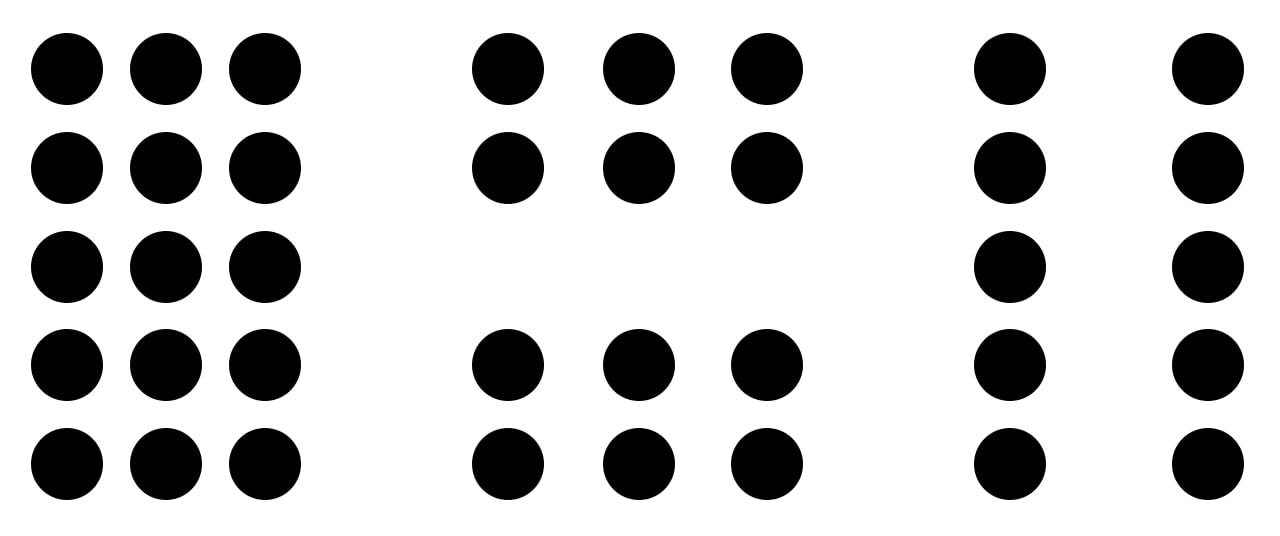
\includegraphics[width=.95\linewidth]{img/gNaehe}  
  \caption{Schematische Darstellung zur Nähe}
  \label{fig:naeheSchema}
\end{subfigure}
\begin{subfigure}{.5\linewidth}
  \centering
  % include second image
  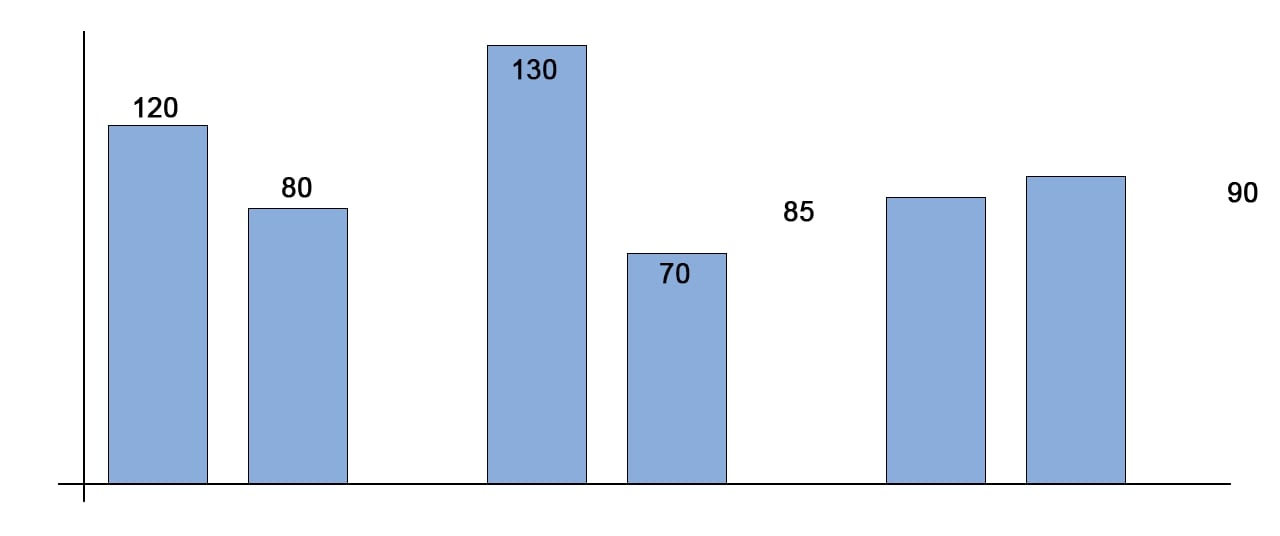
\includegraphics[width=.95\linewidth]{img/gNaeheDia}  
  \caption{Beispiel an einem Balkendiagramm mit zwei positiven und einem negativen (rechts) Beispiel}
  \label{fig:naeheDia}
\end{subfigure}
\caption[Gesetz der Nähe]{Darstellung des Gesetzes der Nähe. Links schematisch und rechts an einem Balkendiagramm dargestellt. Bildquelle: Eigene Darstellung}
\label{fig:naehe}
\end{figure}
%\bild
%{gNaehe}
%{8cm}
%{Beispiel des Gesetzes der Nähe. Eigene Darstellung}
%{Gesetz der Nähe}

Das Gesetz der Nähe besagt, dass Elemente, die nahe beieinander liegen, als eine Einheit wahrgenommen werden.
Dieser Effekt ist in Abbildung \ref{fig:naehe} veranschaulicht.
Für Visualisierungen und insbesondere Diagramme bedeutet dies, dass sich beispielsweise die Zahlen immer in der Nähe des entsprechenden Elements befinden sollten.

In \ref{fig:naeheDia} ist dieser Effekt deutlich zu erkennen. 
Zum einen werden immer zwei Balken aufgrund der Distanz als Zusammengehörig wahrgenommen, zum anderen sind die Zahlen bei den ersten vier Balken gut zuzuordnen.
Bei den letzten zwei Balken sind die Zahlen zu weit entfernt und können den jeweiligen Betrachter verwirren.


\subsubsection{Das Gesetz der Ähnlichkeit}
\label{subsub:ähnlich}
\begin{figure}[ht]
\begin{subfigure}{.5\linewidth}
  \centering
  % include first image
  
\includegraphics[width=.95\linewidth]{img/gAehnlich}  
  \caption{Schematische Darstellung zur Ähnlichkeit}
  \label{fig:aehnlichSchema}
\end{subfigure}
\begin{subfigure}{.5\linewidth}
  \centering
  % include second image
  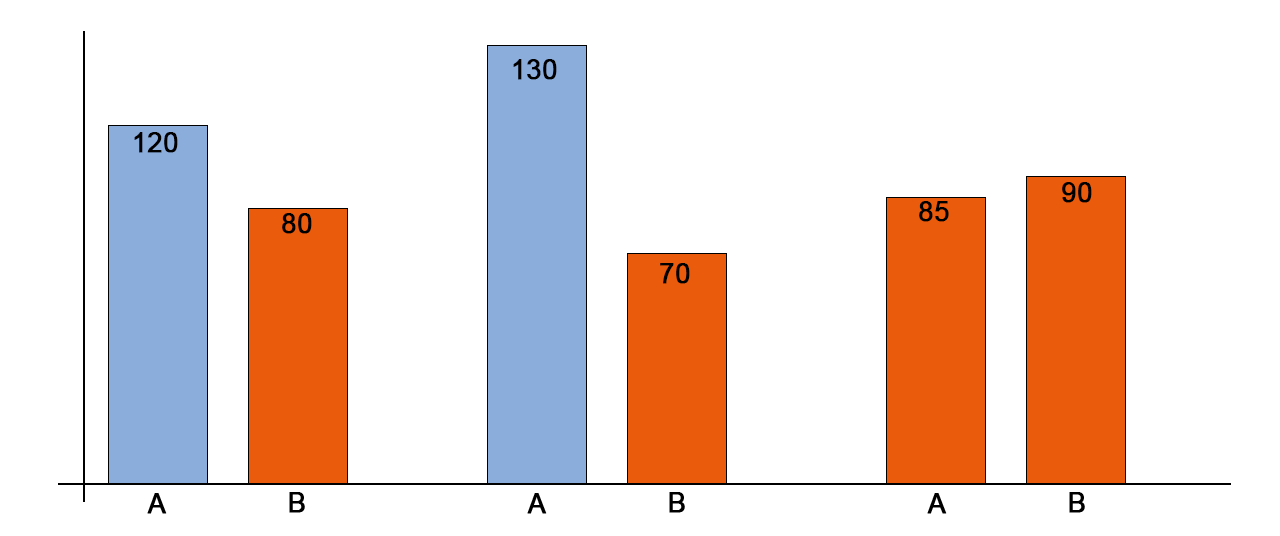
\includegraphics[width=.95\linewidth]{img/gAehnlichDia}  
  \caption{Beispiel an einem Balkendiagramm mit zwei positiven und einem negativen (rechts) Beispiel}
  \label{fig:aehnlichDia}
\end{subfigure}
\caption[Gesetz der Ähnlichkeit]{Darstellung des Gesetzes der Ähnlichkeit. Links schematisch und rechts an einem Balkendiagramm dargestellt. Bildquelle: Eigene Darstellung}
\label{fig:aehnlich}
\end{figure}

Ebenfalls als eine Gruppe werden Elemente wahrgenommen, die ähnlich oder gleich aussehen.
Dabei spielen unterschiedliche Attribute wie Größe, Form oder Farbe eine Rolle.
Hier gilt, je mehr Ähnlichkeit die Elemente besitzen, desto stärker wirken sie als Einheit.

An einem Balkendiagramm ist dieses Gesetz in \ref{fig:aehnlichDia} dargestellt.
Die blauen und orangefarbenen Balken werden als Teile einer Gruppe wahrgenommen.
Die letzten beiden Balken verdeutlichen wieder ein Negativ-Beispiel: Hier werden die Balken fälschlicherweise einer Gruppe zugeordnet, obwohl sie zu zwei unterschiedlichen Gruppen gehören.
Hier wirkt außerdem das Gesetz der Nähe.


\subsubsection{Das Gesetz der Geschlossenheit}
\bild
{gGeschlossenheit}
{8cm}
{Beispiel des Gesetzes der Geschlossenheit. Bildquelle: Eigene Darstellung}
{Gesetz der Geschlossenheit}

Das Gesetz der Geschlossenheit besagt, dass Strukturen und Formen notorisch vervollständigt werden.
Außerdem werden die vervollständigten Formen als eine zusammengehörige Gruppe wahrgenommen.

\subsubsection{Das Gesetz der Erfahrung}
\begin{figure}[ht]
\begin{subfigure}{.5\linewidth}
  \centering
  % include first image
  
\includegraphics[width=.95\linewidth]{img/gErfahrung}  
  \caption{Vervollständigung des Wortes \glqq Erfahrung\grqq}
  \label{fig:erfahrung1}
\end{subfigure}
\begin{subfigure}{.5\linewidth}
  \centering
  % include second image
  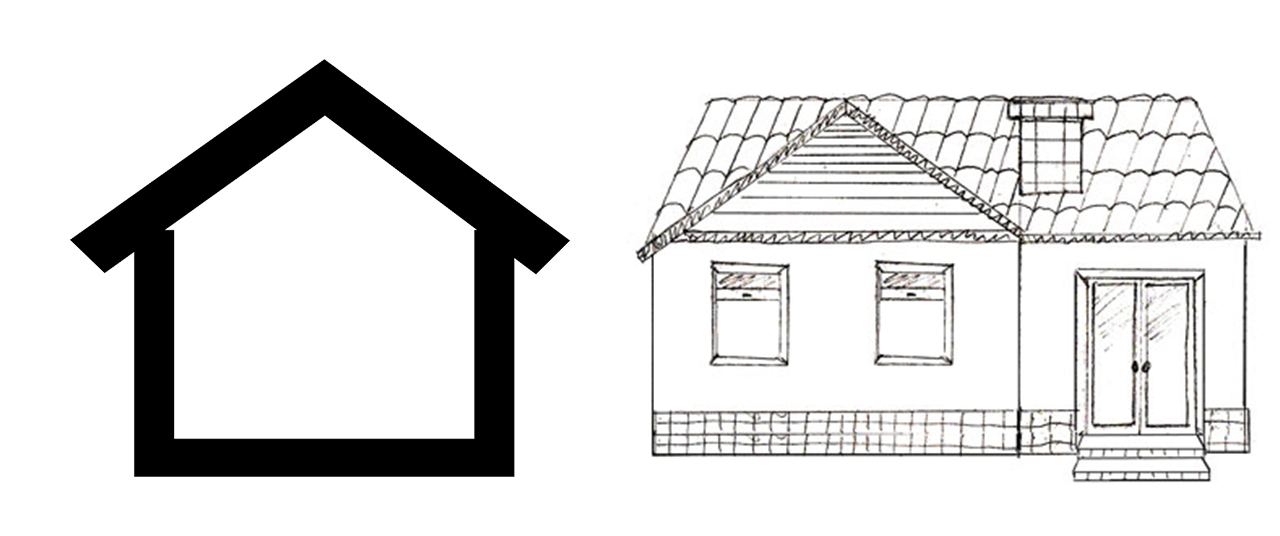
\includegraphics[width=.95\linewidth]{img/gErfahrung2}  
  \caption{Ein minimalistisches (links) und ein detailliertes Haus rechts (Bildquelle: \cite{yedraw.}). Beide sind sofort zu erkennen}
  \label{fig:erfahrung2}
\end{subfigure}
\caption[Gesetz der Erfahrung]{Darstellung des Gesetzes der Erfahrung. Bildquelle: Eigene Darstellung}
\label{fig:erfahrung}
\end{figure}
Das Gesetz der Erfahrung, oftmals auch der Einfachheit oder guten Gestalt genannt, bewirkt, dass unbekannte Objekte stets mit bereits bekannten Objekten abstrahiert werden.
Auch können verdeckte Texte wie in \ref{fig:erfahrung1} trotz fehlender teile gelesen werden.
Doch wenn zu viel Information verdeckt ist, ist auch keine Abstraktion auf bekannte Objekte möglich.

Bei \ref{fig:erfahrung2} wird deutlich, dass mit minimalen Informationen das Objekt klar wird.
Es sind keine Fenster, Türen, Schornstein oder anderes notwendig, damit das linke Objekt als Haus erkannt wird.

%Einfachheit
%der guten Gestalt}
\subsubsection{Das Gesetz der guten Fortsetzung}
\begin{figure}[ht]
\begin{subfigure}{.5\linewidth}
  \centering
  % include first image
  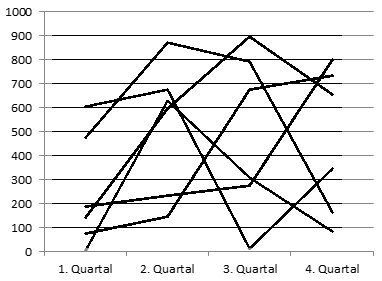
\includegraphics[width=.95\linewidth]{img/gFort}  
  \caption{Ein Liniendiagramm mit vielen schwarzen Linien}
  \label{fig:fort1}
\end{subfigure}
\begin{subfigure}{.5\linewidth}
  \centering
  % include second image
  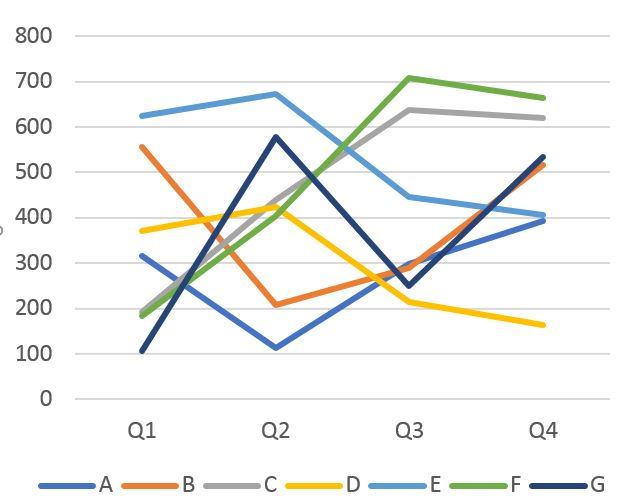
\includegraphics[width=.95\linewidth]{img/gFortC}  
  \caption{Verbesserte Lesbarkeit durch zusätzliches berücksichtigen des Gesetztes der Ähnlichkeit}
  \label{fig:fort2}
\end{subfigure}
\caption[Gesetz der Fortsetzung]{Darstellung des Gesetzes der guten Fortsetzung}
\label{fig:fort}
\end{figure}

Durch das Gesetz der guten oder stetigen Fortsetzung nehmen Menschen beispielsweise kreuzende Formen so wahr, wie sie für uns am einfachsten fortgesetzt werden.
Dies ist insbesondere bei Liniendiagrammen der Fall.

In Abbildung \ref{fig:fort1} sind trotz der vielen gleichfarbigen Linien die Verläufe der einzelnen Kurven dank dieses Prinzips gut erkennbar.
Um jedoch in späteren Anwendungen die Nutzerfreundlichkeit zu erhöhen und Komplexität zu mindern, kann in einem solchen Fall das Gesetz der Ähnlichkeit (siehe \ref{subsub:ähnlich}) zusätzlich angewandt werden.
Die bessere Lesbarkeit ist in \ref{fig:fort2} zu erkennen.

\subsection{Statistische Auswertungen}
\subsubsection{Definition Diagramme}
Wie im zuvor bearbeiteten Kapitel zu sehen ist, wurden als Veranschaulichung der Gestaltungsgrundsätze bereits Diagramme verwendet.
Ein Diagramm ist \glqq eine grafische Darstellung von Größenverhältnissen beziehungsweise Zahlenwerten in anschaulicher, leicht überblickbarer Form\grqq{} (Vgl. \cite{Dudenredaktion.2015}).
Wie in \ref{subsub:visual} bereits untersucht, sind Datenvisualisierungen eine besondere Form von Visualisierung.
Diagramme sind wiederum eine besondere Form der Datenvisualisierung, da sie die fünf Eigenschaften nach \cite{Card.2007} erfüllen, welche eine Datenvisualisierung klassifizieren (siehe S. \pageref{subsub:visual}). 

\subsubsection{(Verschiedene) Arten von Diagrammen und deren Nutzen}
Es gibt dabei eine Vielzahl von Diagrammkategorien, die weit über die klassischen Balken- oder Liniendiagramme hinaus gehen.
Darunter fallen Hyperonyme wie Achsendiagramme, Flussdiagramme (Organigramme), Zeitstrahl, Relationsdiagramme oder spezielle Diagramme in besonderen Fachrichtungen wie ein Klassen(UML)-Diagramm in der Informatik oder ein Grotrian-Diagramm in der Physik \cite{Bounford.2001, Duncan.2018, Engels.2015}.

Im Rahmen dieser Arbeit werden größtenteils die klassischen Achsendiagramme und ein paar spezielle Diagramme beleuchtet.
Dies hängt mit der Intention, der Technologie und den vorliegenden Daten zusammen, da hierfür Kennzahlen und Dimensionen mit- und untereinander in Beziehungen gebracht werden, um neue Erkenntnisse zu erlangen oder Hypothesen zu bearbeiten.

Ein Beispiel dafür, wie effektiv die kognitive Erleichterung durch die grafische Präsentation von Zahlenwerten funktioniert, zeigt das folgende Beispiel:

\begin{table}[htb]
\centering
%\resizebox{\textwidth}{!}{%
\begin{tabular}{|l|l|l|l|}
\hline
\textbf{Kunde}                  & \textbf{Umsatz} & \textbf{Gewinn} & \textbf{Umsatzmarge} \\ \hline
Acer                               & 9.342.856      & 3.513.673             & 37,6\%                     \\ \hline
Boston and Albany Railroad Company & 5.581.529      & 1.924.006             & 34,5\%                     \\ \hline
Calypso                            & 2.327.940      & 1.258.510             & 54,1\%                     \\ \hline
Champion International             & 1.972.009      & 835.208               & 42,4\%                     \\ \hline
Edna Design                        & 2.044.386      & 900.829               & 44,1\%                     \\ \hline
Fokas                              & 1.934.520      & 829.052               & 42,9\%                     \\ \hline
Information Bureau                 & 2.419.778      & 1.097.471             & 45,4\%                     \\ \hline
%J. S. Lee Associates               & 2.048.522      & 263.119               & 12,8\%                     \\ \hline
%KENROB and Associates              & 3.691.399      & 1.671.433             & 45,3\%                     \\ \hline
%Matradi                            & 3.108.910      & 903.906               & 29,1\%                     \\ \hline
%Pacifico                           & 2.248.193      & 464.785               & 20,7\%                     \\ \hline
%Paracel                            & 11.117.286     & 5.077.890             & 45,7\%                     \\ \hline
%Renegade info Crew                 & 1.782.516      & 870.276               & 48,8\%                     \\ \hline
Road Warrior International         & 3.127.719      & 948.304               & 30,3\%                     \\ \hline
Talarian                           & 9.168.719      & 3.281.944             & 35,8\%                     \\ \hline
Tandy Corporation                  & 11.889.136     & 5.585.705             & 47,0\%                     \\ \hline
Target                             & 5.369.579      & 1.711.586             & 31,9\%                     \\ \hline
Teammax                            & 2.009.436      & 1.055.986             & 52,6\%                     \\ \hline
Unison Management Concepts         & 2.115.465      & 1.083.508             & 51,2\%                     \\ \hline
Vanstar                            & 3.720.451      & 1.616.382             & 43,4\%                     \\ \hline
\end{tabular}%
%}
\caption[Beispiel einer Datentabelle]{Ein Beispiel einer Datentabelle mit vier Spalten, mehreren Zeilen und diversen Werten. Herkunft der Daten: Qlik Sense Beispiel-App \glqq Sales Discovery\grqq}
\label{tbl:data}
\end{table}


%booktabs table
%\begin{table}[]
%\centering
%\resizebox{\textwidth}{!}{%
%\begin{tabular}{@{}llll@{}}
%\toprule
%\textbf{Customer}                                        & \textbf{Sales}                  & \textbf{Sales Margin}          & \textbf{Sales Margin (\%)}  \\ \midrule
%\multicolumn{1}{|l|}{Acer}                               & \multicolumn{1}{l|}{9.342.856}  & \multicolumn{1}{l|}{3.513.673} & \multicolumn{1}{l|}{37,6\%} \\ \midrule
%\multicolumn{1}{|l|}{Boston and Albany Railroad Company} & \multicolumn{1}{l|}{5.581.529}  & \multicolumn{1}{l|}{1.924.006} & \multicolumn{1}{l|}{34,5\%} \\ \midrule
%\multicolumn{1}{|l|}{Calypso}                            & \multicolumn{1}{l|}{2.327.940}  & \multicolumn{1}{l|}{1.258.510} & \multicolumn{1}{l|}{54,1\%} \\ \midrule
%\multicolumn{1}{|l|}{Champion International}             & \multicolumn{1}{l|}{1.972.009}  & \multicolumn{1}{l|}{835.208}   & \multicolumn{1}{l|}{42,4\%} \\ \midrule
%\multicolumn{1}{|l|}{Edna Design}                        & \multicolumn{1}{l|}{2.044.386}  & \multicolumn{1}{l|}{900.829}   & \multicolumn{1}{l|}{44,1\%} \\ \midrule
%\multicolumn{1}{|l|}{Fokas}                              & \multicolumn{1}{l|}{1.934.520}  & \multicolumn{1}{l|}{829.052}   & \multicolumn{1}{l|}{42,9\%} \\ \midrule
%\multicolumn{1}{|l|}{Information Bureau}                 & \multicolumn{1}{l|}{2.419.778}  & \multicolumn{1}{l|}{1.097.471} & \multicolumn{1}{l|}{45,4\%} \\ \midrule
%\multicolumn{1}{|l|}{J. S. Lee Associates}               & \multicolumn{1}{l|}{2.048.522}  & \multicolumn{1}{l|}{263.119}   & \multicolumn{1}{l|}{12,8\%} \\ \midrule
%\multicolumn{1}{|l|}{KENROB and Associates}              & \multicolumn{1}{l|}{3.691.399}  & \multicolumn{1}{l|}{1.671.433} & \multicolumn{1}{l|}{45,3\%} \\ \midrule
%\multicolumn{1}{|l|}{Matradi}                            & \multicolumn{1}{l|}{3.108.910}  & \multicolumn{1}{l|}{903.906}   & \multicolumn{1}{l|}{29,1\%} \\ \midrule
%\multicolumn{1}{|l|}{Pacifico}                           & \multicolumn{1}{l|}{2.248.193}  & \multicolumn{1}{l|}{464.785}   & \multicolumn{1}{l|}{20,7\%} \\ \midrule
%\multicolumn{1}{|l|}{Paracel}                            & \multicolumn{1}{l|}{11.117.286} & \multicolumn{1}{l|}{5.077.890} & \multicolumn{1}{l|}{45,7\%} \\ \midrule
%\multicolumn{1}{|l|}{Renegade info Crew}                 & \multicolumn{1}{l|}{1.782.516}  & \multicolumn{1}{l|}{870.276}   & \multicolumn{1}{l|}{48,8\%} \\ \midrule
%\multicolumn{1}{|l|}{Road Warrior International}         & \multicolumn{1}{l|}{3.127.719}  & \multicolumn{1}{l|}{948.304}   & \multicolumn{1}{l|}{30,3\%} \\ \midrule
%\multicolumn{1}{|l|}{Talarian}                           & \multicolumn{1}{l|}{9.168.719}  & \multicolumn{1}{l|}{3.281.944} & \multicolumn{1}{l|}{35,8\%} \\ \midrule
%\multicolumn{1}{|l|}{Tandy Corporation}                  & \multicolumn{1}{l|}{11.889.136} & \multicolumn{1}{l|}{5.585.705} & \multicolumn{1}{l|}{47,0\%} \\ \midrule
%\multicolumn{1}{|l|}{Target}                             & \multicolumn{1}{l|}{5.369.579}  & \multicolumn{1}{l|}{1.711.586} & \multicolumn{1}{l|}{31,9\%} \\ \midrule
%\multicolumn{1}{|l|}{Teammax}                            & \multicolumn{1}{l|}{2.009.436}  & \multicolumn{1}{l|}{1.055.986} & \multicolumn{1}{l|}{52,6\%} \\ \midrule
%\multicolumn{1}{|l|}{Unison Management Concepts}         & \multicolumn{1}{l|}{2.115.465}  & \multicolumn{1}{l|}{1.083.508} & \multicolumn{1}{l|}{51,2\%} \\ \midrule
%Vanstar                                                  & 3.720.451                       & 1.616.382                      & 43,4\%                      \\ \bottomrule
%\end{tabular}%
%}
%\caption{My caption}
%\label{my-label}
%\end{table}

In Tabelle \ref{tbl:data} sind diverse Zahlen zu Kunden und deren Umsätze, Gewinn und Marge zu sehen.
Dabei ist die Informationsflut und daraus resultierende Reizüberflutung für den jeweiligen Betrachter ein Hindernis, um schnell neue Erkenntnisse zu gewinnen oder Vergleiche zu vollziehen.
Welcher Kunde beispielsweise den höchsten oder niedrigsten Umsatz, Gewinn oder Marge hat, ist in dieser Tabelle nicht sofort ersichtlich.

\bildbreit
{MuchDataBetter}
{Die Daten aus Tabelle \ref{tbl:data} in grafischer Form eines Kombinations-Diagrammes dargestellt. Quelle: Qlik Sense Beispiel-App \glqq Sales Discovery\grqq}
{Daten aus Tabelle \ref{tbl:data} in grafischer Form eines Diagrammes dargestellt. }

Eine deutliche Verbesserung der Interpretationsmöglichkeiten ist in Abbildung \ref{fig:MuchDataBetter} zu erkennen.
Hier sind die Daten aus Tabelle \ref{tbl:data} in visueller Form eines dargestellt.
Dabei ist das gewählte Diagramm eine Kombination aus Balken- und Liniendiagramm.

Es ist sofort möglich, den Kunden mit dem meisten und geringsten Umsatz ausfindig zu machen.
Gleichzeitig wird eine Relation des Unterschiedes sichtbar, da die Balkenhöhe gut miteinander verglichen werden kann.
Des Weiteren sind die Zahlen des Gewinnes und der Umsatzmarge als farbig unterscheidbare Striche in den Balken integriert.
Hierdurch sind weitere Beziehung sichtbar, welcher Kunde den höchsten oder niedrigsten Gewinn oder Umsatzmarge generiert.
Auch ist mühelos ein Zusammenhang zwischen Umsatz, Gewinn und Umsatzmarge jedes einzelnen Kunden ersichtlich, welcher wiederum sofort mit anderen Kunden verglichen werden kann.

Die Liste der schnell und effizient identifizierten neuen Erkenntnisse kann noch weiter geführt werden.
Als Motivation und Argument für die grafische Darstellung von solchen Zahlenwerten soll dieser Auszug jedoch genügen.

Eine kurze Auswahl an häufig relevanten Diagrammen und Visualisierungen wird im folgenden kurz erläutert:
\begin{description}
\item[Liniendiagramm] Ein Liniendiagramm ist eine nützliche Visualisierung, um zeitliche Verläufe darzustellen. 
Wenn also temporäre Daten aufgezeigt werden, die eine Veränderung zum nächsten Zeitpunkt aufweisen, kann die Verbindung der Datenpunkte durch Linien eine Abweichung grafisch untermauern. 
Ein Beispiel eines Liniendiagrammes ist in Abbildung \ref{fig:fort2} zu erkennen \cite[S.77]{Engels.2015}.

\item[Balkendiagramm] Balkendiagramme zeigen die absoluten Werte von Daten an und visualisieren eine mögliche Differenz zu anderen Balken \cite[S.54]{Bounford.2001}.
Die Balken gehen dabei üblicherweise von einer gemeinsamen Grundlinie aus, was sie von einem Liniendiagramm unterscheidet.
Dadurch können sehr kleine Änderungen bei großen absoluten Werten unter Umständen untergehen, was bei einem Liniendiagramm nicht der Fall ist, da diese keine Grundlinie bei 0 haben, sondern eine dynamische Y-Achsen-Skalierung nutzen können.

\bild
{kombi}
{14cm}
{Beispiel eines Kombinationsdiagramm aus Balken und einer Linie}
{Kombinationsdiagramm aus Balken und einer Linie}

In einem Kombinationsdiagramm werden in der Regel Balken und Linien oder Symbole miteinander kombiniert, um die Vorteile beider Typen in Anspruch zu nehmen \cite[S.84]{Bounford.2001}.
Hierbei wird in der Regel eine sekundäre Y-Achse an der rechten Seite eines Diagrammes angelegt, welche die Skalierung für die Linie im Balkendiagramm festlegt.
Abbildung \ref{fig:kombi} verdeutlicht die genannten Aspekte.
Zu sehen ist ein Kombinationsdiagramm, dass die absoluten Werte des Budgets als Balken darstellt, und somit jederzeit ein Gefühl für die Gesamtmenge entsteht.
Die Linie repräsentiert dieses hierbei als Prozentangabe mit einer sekundären Achse auf der rechten Seite.
Diese beginnt mit der unteren Grenze von 50\% und kann durch den kleineren Wertebereich minimale Veränderungen zwischen den Monaten viel deutlicher hervorheben.

\item[Flächendiagramm] Das wohl bekannteste Flächendiagramm ist das Kreisdiagramm. 
Es bildet in der Regel eine Dimension und eine Kennzahl ab und zeigt das Verhältnis von einem Objekt zur Gesamtheit \cite[S.72]{Bounford.2001}.
Dabei wird es häufig eingesetzt, um die Vorherrschaft eines bestimmten Objektes gegenüber seinen Konkurrenten zu verdeutlichen.
Auch bei binären Daten bieten sich Kreisdiagramme an, da hierbei das Verhältnis einer Option zur anderen in der Regel interessant ist.

\bild
{kreisdia}
{14cm}
{Darstellung der Wirkungskraft eines Kreisdiagrammes im Vergleich zu einem Balkendiagramm. Herkunft der Daten: Qlik Sense Beispiel-App \glqq Sales Discovery\grqq}
{Darstellung der Wirkungskraft eines Kreisdiagrammes}

Als Beispiel zeigt in Abbildung \ref{fig:kreisdia} das Kreisdiagramm auf der rechten Seite auf einen Blick, dass \glqq ACS Shop\grqq{} mit über der Hälfte des Kreises die absolute Mehrheit der Marktführerschaft besitzt.
Aus dem Balkendiagramm daneben ist diese Überlegenheit auf den ersten Blick nicht garantiert zu erkennen.

%\item[Histogramm] Um die Häufigkeit oder Verteilung bestimmter numerischer Daten zu verlgeichen, werden oftmals Histogramme eingesetzt.
%Diese sind streng genommen eine besondere Form von Balkendiagrammen, da
\item[Boxplot] Ein Boxplot ist ein mächtiges Diagramm, welches eine Vielzahl von Daten in eine kleine \glqq Box\grqq{} packen kann.
Dabei wird um den Mittelwert der vorliegenden Daten zwei Kästen gelegt, welche das oberste und unterste Quartil darstellen.
Somit zeigt die \glqq Box\grqq{}, in welchem Bereich sich 75\% der vorliegenden Daten befinden.
Weiter gibt es sogenannte \glqq Whisker\grqq{}, welche in der Regel maximal 1,5-mal so lang wie die Größe der Box sind. 
Diese sollen das generelle Minimum und Maximum der Daten darstellen.
Optional ist hierbei dann die Anzeige von Ausreißern, welche außerhalb des Bereichs der Whisker liegen \cite[S.59]{FischerStabel.2018}.

\bild
{boxplot}
{14cm}
{Exemplarische Darstellung von einem Boxplot-Diagramm. Gezeigt wird der Anteil an pünktlichen Lieferungen pro Verkäufer verglichen über mehrere Monate}
{Exemplarische Darstellung von einem Boxplot-Diagramm}

Besonders Wirkungsvoll werden Boxplots, wenn zusätzlich eine Gruppe mit unterschiedlichen Daten hierbei verglichen werden kann.
Dies ist exemplarisch in Abbildung \ref{fig:boxplot} dargestellt.
\item[Punktdiagramm] Wenn es um Beziehungen zwischen zwei Kennzahlen geht, ist ein Punktdiagramm das Mittel zum Zweck.
Hier können Beziehungen, Gruppierungen (Cluster), Trends oder andere Strukturen erkannt werden.
Außerdem ist die zusätzliche Einbindung von einer oder zwei Kennzahlen möglich, indem die Größe und/oder Farbe des jeweiligen Punktes entsprechend verändert wird.
So können komplexe Beziehungen aufgedeckt werden, die mittels bloßer Tabellen für einen Mensch kaum ersichtlich sind.
\bildbreit
{punktdia}
{Vergleich von Anzahl der Verkäufe auf der Y-Achse und die prozentuale Marge auf der X-Achse pro Produktkategorie in einem Punktdiagramm. Herkunft der Daten: Qlik Sense Beispiel-App \glqq Sales Discovery\grqq}
{Vergleich von Anzahl der Verkäufe auf der und prozentuale Marge pro Produkt in einem Punktdiagramm}

Ein Beispiel eines solchen Punktdiagrammes ist in Abbildung \ref{fig:punktdia} zu erkennen.
Hier wird beispielsweise deutlich, dass \glqq Canned Foods\grqq{} und \glqq Produce\grqq{} sehr häufig verkauft werden mit einer mittleren Marge, wohingegen \glqq Canned Products\grqq{} und \glqq Seafood\grqq{} sehr selten, aber mit einer hohen Marge verkauft werden.
\end{description}

%\subsection{Multidimensionale Daten darstellen?}

\section{Begriffe zum Thema Data Analytics}
\subsection{Übersicht der Zusammenhänge}

\bild
{interrelations}
{0.8\textwidth}
{Zusammenhänge von Data Analytics, Big Data, Business Intelligence, Data Warehouse und Dashboards visuell dargestellt. Eigene Darstellung, angelehnt an \cite{Dedic.2017}}
{Zusammenhänge von Data Analytics, Big Data, BI, Data Warehouse und Dashboards}

Abbildung \ref{fig:interrelations} verdeutlicht die Abgrenzung und Zusammenhänge der Begrifflichkeiten Data Analytics, Big Data, \gls{BI}, \gls{DWH} und Dashboards.
Demnach ist laut \cite{Dedic.2017} Data Analytics das übergeordnete Konzept, welchem die Bereiche Business Intelligence und Big Data Analytics untergeordnet werden kann.
Dabei kann \gls{BI} eine Big Data Datengrundlage haben, wodurch eine Überschneidung dieser Konzepte zustande kommt.

Außerdem ist bei BI in der Regel ein \gls{DWH} angelegt, was bei Big Data kein Zwang und dementsprechend seltener der Fall ist.
Aus beiden Bereichen können letztendlich Auswertungen betrieben und Einblicke in Daten erlangt werden, welche etwa in Form von Dashboards präsentiert werden.
Die genannten Begrifflichkeiten werden im Folgenden näher erörtert. 
\subsection{Business Intelligence}
\label{sub:bi}
Seit es die Möglichkeit der elektronischen Datenverarbeitung in den 60er Jahren gibt, wird dieses Verfahren genutzt, um betriebswirtschaftliche Daten für Entscheidungen der Managementebene zu verwenden.
Demnach ist es das Ziel, aus vorliegenden Daten Informationen und/oder Erkenntnisse zu gewinnen, die zum Vorteil des jeweiligen Unternehmen beitragen und daraus resultierend ein Wachstum oder verbesserte Performance ermöglichen.
Dabei sind in den Jahrzehnten unterschiedliche Begriffe wie \glqq Management Informationssysteme (MIS)\grqq{} oder \glqq Executive Information System (EIS)\grqq{} für diesen Prozess entstanden (Vgl. \cite[S.3]{Engels.2015}.
Der heutzutage übliche Begriff \acrfull{BI} wurde Anfang der 1990er Jahre durch Howard Dresner eingeführt und populär.
Dieser umfasst dabei zwei wesentliche Bereiche \cite{Kemper.2004}:
\begin{itemize}
\item Die Datenbereitstellung von diversen (oftmals betriebswirtschaftlichen) Kennzahlen. 
Auch deren effiziente Haltung und entsprechende Abfragen zählen zu dieser Rubrik.
Dies umfasst somit den technischen Bereich von \gls{BI}
\item Betriebswirtschaftliche Anwendung, beispielsweise in Form von Unternehmensanalysen 
\end{itemize}

\subsection{Big Data}
\label{sub:bigdata}
\epigraph{\glqq We are drowning in information, but starved for knowledge\grqq}{John Naisbitt, Zukunftsforscher \cite{Naisbitt.1982}}
Dieses Zitat beschreibt die heutige Situation mit dem Verlangen der Menschheit nach Wissen, jedoch das gleichzeitige Untergehen in der Masse an Informationen sehr gut. 
Dabei stammt dieser Satz von einem Zukunftsforscher aus den 80er Jahren.

Big Data (\glqq große Datenmengen\grqq) ist ein Begriff, welcher in den letzten Jahren immer häufiger verwendet wird.
Hierbei handelt es sich um größtenteils un- oder polystrukturierte Daten, welche durch viele unterschiedliche Datenquellen erzeugt werden.
Das Fortschreiten der vielen Digitalisierungsprozesse weltweit führt zu einer stetig stärker wachsenden Datengrundlage. 

\bildbreit
{bigDataPrognose}
%{10cm}
{Prognose zur jährlich generierten digitalen Datenmenge in Zettabyte. Im Vergleich die Prognosen zu den Jahren 2018 und 2025. Bildquelle \cite[S.6]{Reinsel.November2018}}
{Prognose zur jährlich generierten digitalen Datenmenge}

Abbildung \ref{fig:bigDataPrognose} zeigt eine Prognose von Statista, welche die Menge des jährlich generierten Datenvolumens prognostiziert.
Dort ist für das Jahr 2018 ein Volumen von 33 Zettabyte\footnote{ 1 Zettabyte (ZB) = 10\textsuperscript{21} Byte = 1 Milliarde Terabyte (TB) \\
33 ZB pro Jahr entspricht pro Sekunde einer Datenmenge von ca. 1000 TB oder 1 Mio. Gigabyte (GB) \\
175 ZB pro Jahr $\approx$ 5,3 Mio. GB pro Sekunde} prognostiziert.
Für 2025 ist eine Steigerung um mehr als das Fünffache vorausgesehen.

Bei Big Data ist oftmals die Rede der drei A`s, welche den Umfang hiervon beschreiben (Vgl. \cite[2.1]{Hausler.2018}):
\begin{itemize}
\item Aggregation
\item Analyse
\item Auswertung
\end{itemize}
Somit ist nicht nur das Sammeln und Aggregieren großer Datenmengen die Aufgabe von Big Data, wie es oftmals angenommen wird.
Sondern auch die Analyse und das anschließende Auswerten dieser Daten obliegt dieser Begrifflichkeit.


Darüber hinaus gibt es drei V`s, welche die Eigenschaften von Big Data klassifizieren sollen:
\begin{description}
\item[Volume] Kennzeichnet das \glqq Big\grqq{} in Big Data und beschreibt somit das große Volumen der Datenmengen
\item[Velocity] Da die große Masse an Daten in der Regel in einem kontinuierlichen Fluss oder zumindest einer regelmäßigen Zeit generiert werden, ist eine schnelle bis echtzeitnahe Verarbeitung dieser Daten notwendig 
\item[Variety] Die Varietät wird durch eine große Vielfalt der Daten gegeben.
So sind die Daten einer Big Data Anwendung in der Regel unterschiedlichsten Ursprungs. 
Eine Sammlung von Texten, Zahlen, Bildern unterschiedlichen Formats, oftmals auch Audio- oder Videodaten sind demnach klassische Anhäufungen. 
\end{description}


\subsection{Data Warehousing}
\label{sub:warehouse}
Da für diverse Analysen in der heutigen Zeit unterschiedliche Datenformate und Datenquellen herangezogen werden, ist eine effiziente Synthese und Speicherung vonnöten.
Dieser Prozess wird gemeinhin als \glqq Data-Warehousing\grqq{} bezeichnet \cite[S.7]{Gabriel.2011}.

Ein \gls{DWH} ist demnach von den operationellen Datenbanken eine logisch getrennte Datenhaltung.
Dabei soll sie nach \cite[S.6]{Mucksch.2000} möglichst eine unternehmens- oder produktweite Abbildung von relevanten Daten darstellen \cite{Kemper.2004}.



%cubes?

\subsection{Dashboards}
\label{sub:dashboards}
Um stets eine Vielzahl an relevanten Kennzahlen oder Daten im Blick zu haben, wurde ein Prinzip aus der Luftfahrt angewandt.
Dort gibt es im Cockpit eine Anzeigentafel, welche diverse Parameter des Flugobjektes anzeigt.
Eine solche Tafel wird in der Datenanalyse und im \gls{BI} analog verwendet.
Dementsprechend gibt es hierbei häufig \glqq Management Cockpits\grqq{} oder \glqq Dashboards\grqq.
Sie sollen wie die Anzeigen im Flugzeug die wichtigsten Parameter respektive Daten auf einen kurzen Blick erkennbar machen und interpretierbar sein \cite[S.18]{Engels.2015}.

\bildbreit
{exampleDashboard}
{Beispiel eines Dashboards zu einem Verbrauchsgüter-Unternehmen. Qlik-App von den Beispiel-Apps in Qlik Sense Desktop}
{Beispiel eines Dashboards zu einem Verbrauchsgüter-Unternehmen}

Ein solches Dashboard ist in Abbildung \ref{fig:exampleDashboard} dargestellt.
Hier werden exemplarisch die wichtigsten Kennzahlen eines Unternehmens präsentiert.
Somit ist auf einen Blick eine Übersicht und eine Veränderung der Daten zu erkennen.


\section{Daten und deren Verarbeitung in der Notfallmedizin} % Rettungsdienst  
Die zugrundeliegenden Daten dieser Arbeit sind zu einem großen Teil medizinische Daten.
Diese haben nicht nur strenge Regularien, sondern sind auch von besonderer Bedeutung.
So kann unterschiedliche Forschung auf Basis von medizinischen Daten betrieben werden, welche hilft, die Methoden und Praktiken zu verbessern.

Hierbei gilt die Besonderheit, dass die vorliegenden Daten aus dem Bereich der Notfallmedizin stammen.
Demnach gibt es oftmals diverse Daten nicht zuverlässig, die beispielsweise eine Auswertung über Auswirkungen von Medikationen oder Umwelteinflüssen auf den Patienten ermöglichen.
Jedoch stehen auf der anderen Seite Daten zur Verfügung, welche in den wenigsten Bereichen der Medizin generiert oder verfügbar sind.
Ein Beispiel hierfür wären Reanimationsdaten, insbesondere zur Reanimationsqualität, welche beispielsweise Rückschlüsse über unterschiedliche Maßnahmen und deren Auswirkungen ermöglichen.

\subsection{Business Intelligence in der Notfallmedizin}
Der Bereich \gls{BI} ist in der Notfallmedizin ein wichtiger, jedoch nicht stark vertretener Sektor.
So können unterschiedlichste Auswertungen zu betriebswirtschaftlichen Zahlen betrieben werden, die einen positiven Einfluss auf die Prozesse haben können.
Ein Beispiel hierfür ist unter anderem die Ressourcenplanung, welche sowohl die Güter als auch die personellen Ressourcen inkludiert.

Im Rettungswesen müssen diverse Vorgaben und Richtlinien eingehalten werden, welche zum Beispiel durch eine effiziente und vorausschauende Planung erfüllt werden können.
Hierfür eignen sich die Methoden von \gls{BI} aus wirtschaftlichen Unternehmen, wenn sie an entsprechende Prozesse des Gesundheits- und Rettungswesen angepasst werden.

%\todotext{mehr?}

\subsection{Big Data in der Notfallmedizin}

Auch im Gesundheitswesen ist die Zunahme der Datenmengen der letzten Jahre zu spüren.
Dementsprechend ist \glqq Big Data\grqq{} auch hier ein Thema, welches berücksichtigt und im besten Fall genutzt werden sollte, um einen Mehrwert aus den großen Datenmengen zu gewinnen.

\bild
{bigDataGW}
{13cm}
{Prognose zu Big Data im Gesundheitswesen nach Häusler. Deutlich ist die Zunahme an unstrukturierten Daten. Bildquelle: \cite[S.45]{Hausler.2018}}
{Prognose zu Big Data im Gesundheitswesen nach Häusler}

In Abbildung \ref{fig:bigDataGW} ist der Wachstum an Daten im Gesundheitswesen exemplarisch prognostiziert.
Sehr deutlich wird hierbei der Zuwachs an unstrukturierten Daten, welche eine besondere Datenverarbeitung notwendig machen, um aus Ihnen Informationen und digitales Wissen zu erlangen.

Im Gesundheitswesen gelten auch die drei \glqq V`s\grqq{} (siehe \ref{sub:bigdata}), welche die Eigenschaften von Big Data klassifizieren sollen.
Demnach ist beispielsweise die \glqq Velocity\grqq{} ein wichtiger Faktor, wenn es um zeitkritische Daten geht, bei denen die Bearbeitung der Daten Auswirkungen auf einen Patienten haben kann.

Jedoch kommt hier das üblicherweise selten genannte vierte V hinzu: Veracity \cite{Hausler.2018}.
Dieses hat einen besonders hohen Stellenwert im Bereich von medizinischen Daten.
Wörtlich übersetzt bedeutet es \glqq Richtigkeit\grqq{}, wobei Daten als solche nicht richtig oder falsch sein können.
Sie sind von sich aus objektiv und erst im Kontext respektive mit den richtigen Fragestellungen können Daten von hoher oder minderer Qualität sein \cite[S.2 ff]{Gitelman.2013}.
Demnach ist die Richtigkeit der zugrundeliegenden Fragestellungen von besonderer Bedeutung im Rahmen von Daten mit medizinischem Hintergrund \cite[2.1]{Hausler.2018}.
Dies ist unter anderem Grundlage und Motivation für eine umfangreiche Erhebung und Analyse der zu beantwortenden Fragestellungen (siehe \fullref{kap:anforderungsanalyse}).


% MAYBE IF NEEDED MORE TEXT
%Datenquellen (relevanten Auszug davon hervorheben)(S.43f); 
%
%%\begin{table}[hbt]
%%\centering
%%\caption{My caption}
%%\label{my-label}
%%\begin{tabular}{|l|l|} 
%%\hline
%%\textbf{Kategorie der Datenquelle}  & \textbf{Ausgewählte Datenquellen}                                                \\ 
%%\hline
%%Medizinische Daten                  & \begin{tabular}[c]{@{}l@{}}Vitalparameter\\ Länge des Aufenthalts \end{tabular}  \\ 
%%\hline
%%Versicherungsdaten                  & \begin{tabular}[c]{@{}l@{}}Alter\\ Name \end{tabular}                            \\ 
%%\hline
%%Öffentliche Gesundheitsdaten        & \begin{tabular}[c]{@{}l@{}}Ämter\\Gemeinden\\...\end{tabular}                    \\ 
%%\hline
%%Forschungsdaten                     & \begin{tabular}[c]{@{}l@{}}Studien\\Biobanken\end{tabular}                       \\ 
%%\hline
%%Individ. Daten                      & \begin{tabular}[c]{@{}l@{}}Ernährung\\Wellness\end{tabular}                      \\ 
%%\hline
%%Pharmadaten                         & \begin{tabular}[c]{@{}l@{}}Medikamente\\Beschwerden\end{tabular}                 \\ 
%%\hline
%%Nichtklassische Ges.DAten           & \begin{tabular}[c]{@{}l@{}}Meinungen\\Telekomm.\end{tabular}                     \\
%%\hline
%%\end{tabular}
%%\end{table}
%
%strukturiert, un- \& polystrukturiert (S.45): 
%unstrukturiert: MRT, Röntgen, Studien,....
%polystruk.: Grundlage für Big Data; bspw. Laborwerte mit SocialMedia, ...
%img Statista\\
%
%
%Anwendungsmöglichkeiten (S.46ff and BMG S.60ff) Epidemiologie, Epidemieprognose und Gesundheitsmonitoring: Überwachung von Krankheitsbildern, Symptome und Ursachen dieser. Verschiedene Studien, wie Engpässe der Ärzte durch Krankheuitsprognosen, Krebsrisiko durch lokale Luft u.a., oder NAKO Deutschland: neue Erkenntnisse über Volkskrankheiten, Risiken und Symptome. Prognose auch durch Verkehrswege, Luft und Frachtschiffverkehr, ... und weiter audh soziale Faktoren.
%Gesundheitsprävention: Vorhersgaen durch z.B. Wetter und Gebiete, und individuelles Krankheitsbild von einem Patienten. Warnungen um vorzubeugen, Allergien und Asthmathiker, Pollenflüge, bestimmte Orte zu bestimmten Zeiten warnen.
%Entscheidungsunterstützung: Auswertung von z.B. Tumordaten wie Gene und Proteine mit anderen um die Wirksamkeit verschiedener Medikamente zu überprüfen und anschließend ein geeignetes auszuwählen. Aber auch kleinere Entscheidungen (hier für uns / postum),
%(Versorgungs-)Forschung: Unterstützung der bisherigen Forschungen mittels neuer Daten, auch Alltagsdaten oder andere med. Daten. , auch indiv. Patientenbehandlung mit Tumordaten etc.
%Leistungs- und Qualitätsbeurteilung: Messung/Bewertung  der Usetzung von Vorgaben und Leitlinien ( §137 SGB V ? ) und Qualität, auch Behandlungen bewerten oder permanente Überachung von z.B. neugeborneren (Miskad/abernethy 2018) (Für uns sehr relevant!)
%Betrugsbekämpfung: Missbrauch, Falschabrechnungen und Betrug, Medikamtentenmissbrauch,
%(Interne) Prozessverbesserung: Für uns auch serh relelvatn; Personalplanung, Marketing, Controlling; AP-HP Frankreich -> Vorhersage über Patienten aufgund von Krankenhausdaten
%\\
%
%Limitationen(S.51) Auswahl des geeigneten Datensatzes, bzw. Wissen über die Limitation des DS, ! Auswahl der geeigneten Fragestellung, Analyseziel für gegebenen Datensatz !\\
%
%Ausblick (S.53)  Deutscher Ethikrat 2017 Big data und Gesundheit; Islam, n.t. 2017: provably secure -> Auch gut für meinen Ausblick und besonders rechtliche Aspekte!\\ \\
%
%
%S.68, 74, 77 Fotos Handy\\ \\
%
%
%S.101ff, 116ff Fotos

%%Done
%%Noch umschreiben! Fast 100% aus Buch
%3A: Aggregation, Analyse, Auswertung
%4V: Volume, Varierty, Velocity \& !med wichtig Veracity! 
%Grundsätzlich nur 3V, aber Veracity ist im GEsundheitsweesen von besonderer Bedeutung. 
%Volume Viele Daten: Statista DAtenvolumen.
%Variety: Häufig unstrukturiert, Papier, Memo, Blog, Freteixt; Im GW besonder Rezepte, Arztmemos, Arztbriefe, Emails
%Velocity: Geschwindigkeit auch wichig, besonders auch in GW, zb. weitere Befunde/ANalysen während initialer Diagnose oder erste Behandlung...
%Veracity: DAten sind per se nicht gut/sclhect, qualitativ hochwertig oder mangelhaft. Daten sind neutral, wenn auch komplex sozial und technologisch Ref Gitelmann 2ff.Entscheidend ist die richtige Fragstellung im Kontext und Algorithmus. Qualitativ hochwertige Bearbeitung der Daten! \\

%% Vermutlich nicht
%eHealth <-> Big Data (S.37f)
%eHealth beschreibt Interface, welches mittels App, online-Plattform,... gesundheitsbezogene Dienstleistungen zur verfügung stellt, Menschen miteineander verbindet eoder technoglogische Erkenntnisse für Menschen sichtbart macht. 
%- ehealth Endgeräteübergreifend, mHealth nur mobile, vHealth VR, aHealth Augemnted
%- eHealth bietet Basis für Big Data, Big Data bietet Basis für eHealth, ...; nicht alles was ehealth ist, ist big data and vice versa; Trennung notwendig! picture\\

\section{Requirements Engineering}
Requirements Engineering, zu deutsch Anforderungstechnik, beschreibt primär den Prozess, Anforderungen zu sammeln und zu spezifizieren.
Dabei gibt es mehrere Orientierungen, welche die Definition variieren lassen: technisch, nutzer- oder risikoorientiert \cite{Glinz.2005, Sommerville.2012}.

Bei der technischen Definition geht es um das Erfassen, Beschreiben und Prüfen von Anforderungen an ein System.
Dabei wird im ersten Schritt bei einer Software eine Reihe an Anforderungen festgehalten, die das System erfüllen sollte.
Hier liegt oftmals der Schwerpunkt in den technischen Details.

Bei der nutzerorientierten Herangehensweise steht, wie der Name suggeriert, der spätere Anwender im Mittelpunkt. 
Hier werden spezifische Anforderungen der Stakeholder gesammelt, spezifiziert und analysiert.
Dies spiegelt eine menschzentrierte Entwicklung wider.

Die risikoorientierte Anforderungstechnik ist ähnlich zu der Vorigen, mit dem Unterschied in der Definition.
Hierbei soll das Risiko, dass die Software dem Anwender keine oder wenig Vorteile bringt oder nicht gefällt, minimiert werden.

\subsection{Methodik}
\label{sub:methodik}
Eine standardmäßige Methodik beim \gls{RE} ist eine iterative Herangehensweise \cite{Pohl.2011}.
Demnach werden die verschiedenen Stationen des \gls{RE} in zyklischen Iterationen durchgeführt (siehe S. \pageref{fig:requireEngineering}, Abbildung \ref{fig:requireEngineering}).

Im Rahmen dieser Arbeit wird die aus dem vorigen Kapitel zweite Definition, die nutzerorientierte Anforderungstechnik, angewandt. 

Eine genaue Beschreibung, welche Schritte in welcher Reihenfolge und mit welchen Methodiken durchgeführt werden, ist Kapitel \ref{sec:erhebung} zu entnehmen.
 
 
\section{Technologien}
\subsection{Qlik Sense}
\label{sub:qlik}
%\todo{add citavi qlik site}
Die Haupttechnologie dieser Arbeit ist Qlik Sense.
Dies ist eine webbasierte Business-Intelligence-Software der Firma QlikTech, welche mit HTML und JavaScript umgesetzt ist.
Die Informationen stammen aus eigener Erfahrung und von dem Web-Auftritt \cite{QlikTech.2019} des Unternehmens. 
Es gibt sowohl eine kostenfreie Variante Qlik Sense Desktop für private Nutzer als auch eine Cloud- oder Enterprise-Variante, welche in \ref{subsub:enterprise} näher beschrieben wird.

Qlik basiert dabei auf sogenannten \glqq Apps\grqq{}, welche ein abgegrenztes Datenmodell und mehrere Arbeitsblätter enthalten.
Dabei steht ein Arbeitsblatt in der Regel für ein \gls{Dashboard}, welches zusammengehörige Visualisierungen auf einen Blick kombiniert.

%\bildbreit
%{qlikstart}
%{Beispielhafte Startseite von Qlik Sense Desktop mit diversen Apps}
%{Startseite von Qlik mit diversen Apps}

Es gibt außerdem die Funktion von Master-Elementen.
Hierbei können Master-Kennzahlen und -Dimensionen aus den Datenfeldern der Tabellen erstellt werden. 
So können diverse Aggregationen oder sonstige Prozesse vorgenommen werden, um die Darstellung in Diagrammen zu ermöglichen.
Diese können wiederum auch als Master-Visualisierung abgespeichert werden.
Ein großer Vorteil dieser Master-Elemente ist die zentrale Verwaltung und damit parallele Manipulation von diversen Visualisierungen, Kennzahlen oder Dimensionen.

Ein weiteres Merkmal von Qlik Sense ist die hohe Interaktion mit den Diagrammen.
So können durch Mausinteraktionen mit den entsprechenden Darstellungen interagiert und eine intuitive Filterung der Daten vorgenommen werden.

Es gibt einen jährlichen Report für \gls{BI} \& Analytics Plattformen von Gartner, welcher die verschiedenen BI-Werkzeuge analysiert, bewertet und anschließend kategorisiert.
Dabei entsteht das sogenannte \glqq Magic Quadrant\grqq{} von Gartner.
\bild
{gartner}
{10cm}
{Magisches Quadrant von Gartner zur Beurteilung verschiedener Business-Intelligence Plattformen. Bildquelle \cite{Howson.Februar2019}}
{Quadrant von Gartner zur Beurteilung verschiedener BI-Plattformen}

Dabei werden die Produkte in vier Quadranten eingeteilt: Leader, Challenger, Visionaries \& Niche Players.
Die Einordnung basiert dabei auf der Vollständigkeit der Vision sowie der Fähigkeit, diese umsetzen zu können \cite{Howson.Februar2019}.
Qlik ist hierbei im aktuellen Jahre 2019 im Quadrant der \glqq Leader\grqq{} mit nur drei weiteren Plattformen, wie Abbildung \ref{fig:gartner} zeigt.
Seit neun Jahren in Folge liegt Qlik in diesem obersten Quadranten \cite{QlikTech.2019}.

\subsubsection{Qlik Sense-Skriptsprache}
Die Syntax von Qlik Sense Skripten basiert auf dem \gls{BNF}. 
%\add citavi: Donald E. Knuth: Backus Normal Form vs. Backus Naur Form. In: Communications of the ACM. Band 7, Nr. 12, 1964, S. 735–737, doi:10.1145/355588.365140.
Demnach gibt es verschiedene Notationen, um sogenannte \glqq Symbole\grqq{} zu definieren.
So ist beispielsweise das Symbol \glqq as\grqq{} mit dem dahinter liegenden Befehl \code{alias fieldname as aliasname \{ , fieldname as aliasname\}} deklariert \cite{QlikTech.Februar2019}.
Dadurch gibt es bereits ein breites Spektrum an den notwendigsten Symbolen, um Daten sinnvoll zu transformieren.

Des Weiteren unterstützt die Skriptsprache diverse Steuerungsbefehle wie If-Bedingungen oder For-Schleifen mittels logischen Operatoren, Deklarieren und Verändern von Variablen und beendet einen Befehl mit einem Semikolon.
Diverse weitere Befehle wie \glqq Join\grqq{} oder \glqq Concatenate\grqq{} gehören zu den Standard-Befehlen, um schnell und effizient Daten zu manipulieren.

\subsubsection{Qlik Sense Enterprise}
\label{subsub:enterprise}
Für größere Teams ab fünf Personen\footnote{Grenze der kollaborativen Funktionen der kostenfreien Version von Qlik Sense} gibt es die kostenpflichtige Steigerung von Qlik Sense Desktop: Qlik Sense Cloud \cite{QlikTech.2019}.
Hierbei können die Apps und deren Visualisierungen mit mehr als fünf Personen geteilt werden und so eine ortsunabhängige Kollaboration ermöglichen.

Die nächste und damit höchste Stufe bildet Qlik Sense Enterprise.
Dieses Produkt ist für große Unternehmen oder solche, die es als Komponente in ihren eigenen Produkten verwenden (\gls{OEM}).
Da \gls{ANALYSE} um ein solches Feature der visuellen \gls{BI}-Analyse erweitert werden soll, ist \gls{GS} Kunde von QlikTech mit dem Produkt Qlik Sense Enterprise im \gls{OEM}-Modell.

Hierbei ist unter anderem eine Benutzerverwaltung mit Rechtesystem mit im Umfang.
So können die bisherigen Benutzersysteme der  \textsf{corpuls\color{corpulsred}{.web}}-Familie in Qlik abgebildet werden.
Auch ist so eine Rechteverteilung denkbar, sodass verschiedene Dashboards nur bestimmten Nutzergruppen zugänglich ist (Administratoren, Forscher und andere).

%\subsubsection{Lizenzierungsmodell}

\section{Ist-Zustand \acrlong*{ANALYSE}}
\label{sec:istAnalyse}
Die \textsf{corpuls\color{corpulsred}{.web}}-Produktfamilie stellt den Zusammenschluss der Softwareprodukte von \gls{GS} dar.
Die für diese Arbeit relevanten Softwareprodukte sind \gls{REVIEW} und insbesondere \acrfull{ANALYSE}, wobei der aktuelle Stand der Technik für letzteres im Folgenden näher erläutert wird.

\gls{REVIEW} wird hauptsächlich in der präklinischen Rettung, beispielsweise einer Rettungswache, ansonsten auch in der klinischen Umgebung wie der Notaufnahme verwendet.
Es dient dabei dem Nachvollziehen einer Mission im Detail.

\gls{ANALYSE} ist eine Erweiterung als Server, welcher per Upload oder Import alle Einsätze abspeichert. 
Mithilfe einer Suchmaske können in einer Tabelle entsprechende Einsätze nach bestimmten Kriterien gesucht und gefiltert werden.
Ein Ausschnitt dieser Tabelle mit Suchmaske ist der Abbildung \ref{fig:missionlist} zu entnehmen.
Anschließend kann ein Einsatz in \gls{REVIEW} geöffnet und im Detail betrachtet werden.

\bildbreit
{missionlist}
{Ausschnitt aus der \glqq Missionsliste\grqq{} in \acrlong*{ANALYSE}}
{Missionsliste in \acrlong*{ANALYSE}}


\subsection{Vorliegende Daten der Geräte}
Im Server von \gls{ANALYSE} liegen die Einsätze in einer Datenbank (MongoDB).
Dort werden alle zugehörigen Komponenten wie beispielsweise Events, \gls{EKG}-Daten oder \gls{MM} in einem Einsatz-Objekt abgespeichert.

Ein Event ist ein Ereignis im Laufe einer Mission, welche mit einer ID und entsprechenden Parametern abgespeichert wird.
Dabei gibt es die Unterscheidung zwischen Benutzer- und Hersteller-Events.
Hersteller-Events umfassen jegliche Interaktion mit und Meldungen vom Gerät, sodass beispielsweise jeder Tastendruck mit einer genauen Uhrzeit nachvollzogen werden kann.
Benutzer-Events sind Ereignisse, welche für die Anwender interessant sind. 
Darunter zählen etwa das Abgeben einer Defibrillation, Auftreten eines Alarmes oder das Versenden eines \gls{EKG}s.

Ein \gls{MM} ist ein Feld, welches bestimmte Events zusammenfasst.
So ist beispielsweise die Aggregation der Defibrillationsereignisse, welche die Abgabe eines solchen aufzeichnen, später als MM für die Anzahl der abgegebenen Defibrillationen in ANALYSE aufzufinden.
Es gibt eine große Sammlung dieser MM, welche im Laufe der Zeit angelegt wurden, um die Kernelemente eines Einsatzes zusammenzufassen.
Diese Felder sind in der Einsatztabelle von ANALYSE zu sehen (Abb. \ref{fig:missionlist}) und auch nur über sie ist eine Suche oder Filterung möglich.


%\subsection{Architektur}
\subsection{Verwendung zur Auswertung}
Das Auswerten von vielen Einsätzen, gegebenenfalls auch mit bestimmten Kriterien wie \glqq nur Nachts\grqq, ist zurzeit bedingt möglich.
Hierfür können entweder die Einsätze in der Tabelle direkt miteinander verglichen werden oder eine Mehrfachauswahl an Einsätzen vorgenommen, siehe Abbildung \ref{fig:missionlist}, und anschließend ein Export im CSV-, BDF+-, oder \glqq corpuls ZIP\grqq -Format durchgeführt werden.
Daraufhin kann mit dem jeweiligen Export in einem Drittanbieterprogramm eine oberflächliche Auswertung der ausgewählten Einsätze vollzogen werden.

Da dies jedoch immer nur auf Basis von den voraggregierten \gls{MM} basiert, ist eine tiefgreifende Analyse der Daten und Einsätze mit deren Ereignissen nicht möglich.
Dies ist unter anderem Aufgabe dieser Arbeit, eine erweiterte Auswertung zu ermöglichen (siehe \ref{sub:erweiterung}).



\chapter{Stand der Technik} 
\label{technikstand]}
\minitoc\pagebreak
%\section{Analyse} Eventuell eigenes Kapitel


\section{Ist-Zustand corpuls.web ANALYSE}
\subsection{Verwendung zur Auswertung}
\subsection{Vorliegende Daten der Geräte}
%\subsection{Anforderungsanalyse ?Eigenes Kapitel?}
%\subsubsection{Nutzergruppen}
%\subsubsection{Aufgabenanalyse}
%\subsubsection{Nutzungskontext}
%\subsubsection{Szenarien}

\section{Qlik Sense Server}
\subsection{Lizenzierungsmodell}
\subsection{?}
\chapter{Anforderungsanalyse}
\label{anforderungsanalyse}
\minitoc\pagebreak
%\section{Requirements Engineering}
% \lipsum[1-52]
\section{Nutzergruppen}
Die unterschiedlichen Nutzergruppen, oftmals auch Benutzerklassen genannt (vgl. \cite[S. 125]{Herczeg.2018}), einer Anwendung sind ein essentieller, beeinflussender Faktor, wenn es um die Entwicklung einer Anwendung oder, wie in dieser Arbeit, die Erweiterung einer Anwendung um ein umfangreiches Feature geht. Sie beschränken, aber auch erweitern die geforderten Funktionalitäten und beeinflussen die Art und Weise, wie die Anwendung gestaltet wird. Beispielsweise welche Erfahrungswerte vorausgesetzt oder angelernt werden müssen, welche Icons oder Symbole bekannt oder unbekannt sind, welche Ziele, Erwartungen oder Befürchtungen sie haben spielen eine große Rolle bei der Entscheidung, welche Informationen in welchem Format dargestellt werden.

\begin{quote}
"`Ein Stakeholder ist eine Person oder Organisation, die einen direkten oder indirekten Einfluss auf die Systemanforderung hat"' \cite{Pohl.2011} 
\end{quote}
Auch eine "`Stakeholder-Liste"' ist ein hilfreiches Mittel, um einen Überblick an den beteiligten Personen zu erhalten und damit einhergehend so viele Anforderungen wie möglich an das System zu erheben (vgl. \cite[S. 83]{Bergsmann.2018}).
Dieser Prozess ist vor allem zu Beginn der Anforderungsanalyse von besonderer Bedeutung, da so frühzeitig viele Informationen und Hinweise erkennbar werden, wie das System aufgebaut werden muss.
Ein nachträgliches anpassen oder hinzufügen von Anforderungen kann unter Umständen schwere grundlegende Probleme mit sich ziehen, da gewisse fundamentale Architekturentscheidung auf der Basis dieser Ansprüche aufbauen können.

Dabei kann grundsätzlich zwischen zwei Gruppen von Stakeholdern unterschieden werden \cite{Leffingwell.2011}:
\begin{description}
\item [Requirements-Provider] \hfill \\
Diese Personen oder Organisationen sind in der Regel jene, welche die Software oder das Produkt im Tagesgeschäft nutzen beziehungsweise voraussichtlich nutzen werden.
Sie haben neue Ideen oder Verbesserungsvorschläge aus vorherigen Anwendungen.
Dies können auch interne Mitarbeiter der Firma sein, welche besondere Erfahrungen in den zu entwickelnden Bereichen haben. %Ref to internal Stakeholders somehow?
\item [Constraint-Provider] \hfill \\
Hierbei handelt es sich um Personen, welche keine Anforderungen als solche definieren, sondern die Umsetzbarkeit der Anforderungen von den Requirements-Providern testen und daraus folgend technische Rahmenbedingungen, wie zum Beispiel die zu verwendende  Programmiersprache oder Datenbank, empfehlen oder festlegen.
\end{description}
\todotext{Referenzierung oder Verbindung zu meinen Nutzergruppen, Stakeholdern. \\Abgrenzung nur Anwender,keine Deployer etc.?, \\ Anforderungen weniger, sondern nur Fragestellungen }

Daher ist zuerst zu klären, welche Nutzergruppen bei dem bisherigen Produkt vertreten sind.
Anschließend sollten diese Benutzerklassen in Hinblick auf das erarbeitende Thema analysiert werden und daraufhin ist zu definieren, welche Eigenschaften oder Charakteristiken diese besitzen und ob gegebenenfalls Neue hinzukommen oder Alte hinfällig sind. 

\subsection{Stakeholder von corpuls.web ANALYSE}

% not sure if I#ll keep this table or just make a Auszug of it and more text?
\begin{table}
\centering
\setlength{\extrarowheight}{4pt}
\begin{tabular}{ | p{0.05\linewidth} | p{0.2\linewidth} | p{0.4\linewidth} | p{0.35\linewidth} |}
  \hline
  \textbf{ID} & \textbf{Stakeholder-Bezeichnung} & \textbf{Organisation} & \textbf{Kontaktperson}
  \\\hline
  1			& Geschäftsführer & GS Elektromedizinische Geräte & Dr. Klimmer
  \\\hline  
  2			& Entwickler & GS Elektromedizinische Geräte & Florian Lehmann
  \\\hline
\end{tabular} 
  \caption[Stakeholder-Liste]{Stakeholder-Liste nach \cite[S. 85]{Bergsmann.2018}}
  \label{tbl:Stakeholder-Liste}
\end{table}



\subsection{Personas}
\section{Aufgabenanalyse}

\section{Nutzungskontext}

\section{Iterative Erhebung der zu beantwortenden Fragestellungen}
\subsection{Ermittlung von Fragestellungen}
\subsection{Analyse der Anforderungen}
\subsection{Spezifikation der Fragen und benötigte Daten}
\subsection{Validierung der spezifizierten Fragestellungen}
\chapter{Konzeption}
\label{kap:konzept}

\minitoc\pagebreak
%\lipsum[1-60]

\section{Vorgehen bei der Konzeption}
\label{sec:vorgehenKonzept}
%\bildrechts{iterative} {2cm} {it} {iter}

Gemäß der Methoden des Requirements Engineering \ref{requireEng} wird anhand der erhobenen und ausgearbeiteten Fragestellungen beziehungsweise Anforderungen aus \ref{4.4 fragestellungen} ein Konzept erarbeitet. 
Auch hierbei wurde eine iterative Herangehensweise gewählt, unter anderem um in einer kurzen Zeit grobe Fehler zu erkennen und viele Verbesserungen herauszufinden. 
Auch wird hierdurch gewährleistet, dass die exemplarischen und später produktiven Auswertungen und Visualisierungen nicht gänzlich in eine falsche Richtung gehen, sondern von Anfang an etwaige Missverständnisse aufgedeckt werden oder grundlegende Entscheidungen frühzeitig überdacht werden können.

Um von vornherein ein realistisches "`Look-and-Feel"' zu bieten und die entsprechend geplante Technologie mit ihren Funktionen und der Nutzerführung zu evaluieren, wird beim Prototyp bereits Qlik Sense \ref{sub:qlik} verwendet. 
Ein weiterer Vorteil ist, dass das notwendige Einarbeiten für die spätere Umsetzung in diese Technologie bereits gewährleistet wird. 
Dabei können auch vorab verschiedene Vor- und Nachteile der Technologie herausgefunden werden und dementsprechend können diese bei der weiteren Planung und Umsetzung berücksichtigt werden, was viel Zeit sparen kann.

Des Weiteren wurden Dummy-Daten unter anderem zum Testen des Prototypen generiert. 
Sie waren auch notwendig, um entsprechend andere Tests für die Datenbank und Auslastung durchzuführen \ref{db und lasttest}. 
Dabei wurde ein Python-Skript geschrieben, welches einige Daten zufällig generiert, jedoch auf einer realistischen Basis.

Die Evaluation soll wie oben beschrieben iterativ sein, was mehrere Termine mit unterschiedlichen Experten zur Konsequenz hat. 
Im Zuge dieser Bachelorarbeit wird die Evaluation des Prototyps mit Mitarbeitern der Firma \gls{GS} durchgeführt. 
Das unternehmen besitzt Abteilungen, in welchen genügend Fachleute sitzen, die in der Lage sind diese Dashboards kritisch prüfen zu können. 
Hierbei wird darauf geachtet, unterschiedliches Personal miteinzubeziehen, sodass es keine exklusive/alleinige Evaluierung durch die Abteilung medizinische Forschung ist, sondern auch Vertriebsmitarbeiter oder andere Stakeholder sollen den Prototyp kritisch untersuchen.

%Bei der Konzeption ist auch das Datenmodell ein wichtiger Bestandteil. 
%Hier können verschiedene Modelle ausprobiert werden und gegebenenfalls Änderungen vorgenommen werden, sollten sich bei der Evaluation Probleme oder andere Anforderungen herausstellen.


\section{Erstellung eines Prototypen}
\label{sec:erstellungPrototyp}
\subsection{Verwendete Technologie}
\label{sub:verweTech}
Für den ersten Prototypen wurde sogleich die letztendlich umsetzende Technologie Qlik Sense \ref{sub:qlik} verwendet. 
Der Einfachheit halber beschränkte sich dies zu Anfang auf Qlik Sense Desktop, einerseits aufgrund der vereinfachten Bedienung, hauptsächlich jedoch da der entsprechende Server mit der Qlik Sense Server Variante zu Anfang der Konzeption noch nicht eingerichtet war. 
Ein Umzug von Qlik Sense Desktop zu Server stellt keine größeren Probleme dar, man kann die erstellten Apps bidirektional ex- und importieren. 
Lediglich die Datenverbindungen, welche für die jeweiligen Applikationen die Daten aus einer Quelle beziehen, werden nicht fehlerlos übertragen.

\subsection{Datengrundlage}
\label{sub:datengrundlage}
Zu Beginn wurde überlegt, welche Daten die Grundlage für den Prototypen bilden sollte.
Dabei wurde auf die Demo-Datenbank des internen \gls{ANALYSE} - Servers zurückgegriffen, welche zu diesem Zeitpunkt in etwa 100.000 Missionen enthielt, von denen jedoch die meisten nur Test-Missionen sind. 
Dies sind solche, die entweder von der internen Testabteilung oder der Software-Entwickler beim Testen von Funktionen oder Herausfinden von Problemen am Gerät oder durch die Software erzeugt werden. 
Dementsprechend enthalten sie wenige spannende Daten, die auch selten realistisch sind und etwaige neue Erkenntnisse nicht darlegen können. 
Nichtsdestotrotz bilden sie eine gute Grundlage um die ersten Basis-Auswertungen von Missionen paradigmatisch darzustellen. 

Für diesen Zweck kann die Export-Funktion im CSV-Format von Analyse genutzt werden, welche in  \ref{istzustandanalysezurauswertung} näher beschrieben ist. 
So war es für den Anfang möglich, einen relativ großen Datensatz mit mäßig sinnvollen Daten zu erhalten.%\footnote{(In späteren Szenarios\ref{lasttests,db} wurden eigens generierte Missionen verwendet. Auf die Erzeugung dieser wird in Kapitel \ref{dummydaten} genauer eingegangen.)}



\subsection{Erstellung exemplarischer Dashboards} 
\label{sub:erstellungDashboards}
Mit der Datengrundlage und der Technologie Qlik Sense Desktop können nun die ersten beispielhaften Dashboards entwickelt werden.
Die Basis für die verschiedenen Diagramme und Auswertungen bilden die iterativ erhobenen Fragestellungen aus Kap \ref{itErhebFrage}. 
Der Ansatz hierbei ist, mit einer grafischen Darstellung der Daten so viele Fragestellungen wie möglich beantworten zu können.
Dabei werden für die Art und Weise der Darstellungen verschiedene Aspekte berücksichtigt, wie zum Beispiel ob es ein zeitlicher Verlauf ist oder tendenziell eine Momentaufnahme, absolute gegen relative Kennzahlen, Veränderungen oder Trends und vieles mehr.
Auf Basis dieser Aspekte wird eine möglichst passende Darstellungsform gewählt und mit entsprechender Dimension und Kennzahl, eventuell auch mehrere Dimensionen und/oder Kennzahlen, gefüllt.

Eine sinnvolle Gruppierung oder Aufteilung der entsprechenden Arbeitsblätter oder Diagramme ist im Zuge des Prototyps von keiner hoher Priorität. 
Im Fokus steht die erstmalige Beantwortung möglichst vieler Fragestellungen, auch gegebenenfalls auf verschiedenen Wegen mit alternativen Darstellungsformen.
Nichtsdestotrotz wird später, zum Zeitpunkt der Evaluierung, eine einigermaßen angebrachte Gruppierung von Diagrammen und vernünftige Reihenfolge der Arbeitsblätter vorgenommen, damit für die entsprechenden Personen eine Struktur erkennbar ist, um mögliche Verwirrungen zu vermeiden.


%\subsubsection{Datenladeskript}
%, Was ist rel, was test, ....
%\subsubsection{Datenmodell}
%recht simpel. im prinzip eine Tabelle, keine Mehrdim, ...
% Vermutlich nur Umsetzung, vielleicht auch hier

%subsubsection Dashboards, und dann unterpunkte?
\subsubsection{Startseite}
\label{subsub:start}
\bildbreit
{Uebersicht_Prototyp}
{Übersicht über die zugrundeliegenden Einsätze}
{Prototyp Überblick-Visualisierungen}

Die erste Seite, die der Kunde zu sehen bekommt wenn er die Software startet, soll ihm einen groben Überblick verschaffen. 
Es ist wie die Startseite einer Website, wo man die wichtigsten Informationen unmittelbar auf der ersten Seite finden kann.
Die Abbildung \ref{fig:Uebersicht_Prototyp} zeigt die erste Version dieser Startseite.

Sie wurde recht simpel mit vier Diagrammen und zwei Kennzahlen gefüllt, damit der erste Eindruck nicht von einer Informationsflut negativ beeinflusst wird.
Sollte der Nutzer weiterführende Informationen und tiefgreifendere Analysen durchführen wollen, kann er diesen Ansprüchen auf den folgenden Dashboards gerecht werden.
%\bildrechts{waterfall} {4cm} {w} {wa}
Das Wasserfall-Diagramm ganz links zeigt die absolute Anzahl an Einsätzen, die all seine Geräte durchgeführt haben.
Des Weiteren werden die absoluten Zahlen der verschiedenen Einsatzarten in Relation zur Gesamtmenge grafisch dargestellt.
Hierbei wird unter anderem zwischen Testeinsätzen, Reanimationen oder sonstigen Einsätzen unterschieden.
Bei den Reanimationen gibt es drei weitere Unterarten: (bulletlist?) Mit \& Ohne Feedbacksensor oder eine mechanische Reanimation.
Die Farbgebung soll Teilsummen von Gesamtmengen unterscheiden.
Ziel der Darstellung ist ein visueller Eindruck, wie viele Einsätze es gibt und welche Arten von Einsätzen in welchem Maße vorkommen.

Das Liniendiagramm stellt den zeitlichen Verlauf der Einsätze dar.
Als (zeitliche) Dimension wurde hier Jahr-Monat gewählt, eine Alternative wäre die tatsächliche Datumsangabe, dies würde jedoch zu einer Kurve führen, welche viele Zacken enthält (Vergleichsbild?) und damit sehr unruhig wirkt.
Die Aufsummierung in Monate, alternativ auch Wochen, bringt je nach Datenlage eine recht glatte Kurve mit sich. 
Die Kennzahlen dieser Visualisierung sind die Summe der relevanten Einsätze und zum Vergleich die Summe der Reanimationen. 
Eine Mini-Legende unterhalb der Grafik erleichtert die Orientierung, sollte der Nutzer in einen bestimmten Zeitraum "`reinzoomen"'.

%Es wurde die AutoCalendar-Funktion genutzt, damit ein fließender Übergang zwischen den Jahren möglich ist.

Darunter sind zwei Kreisdiagramme zu sehen, welche die Anzahl der Einsätze und der Reanimationen pro Gerätetyp anzeigen.
Diese Art der Visualisierung wurde gewählt, damit die Relation und Verteilung unter den Geräten deutlich gemacht wird.
Unter dem jeweiligen Kreisdiagramm ist als einzelner \gls{KPI} die durchschnittliche Einsatz- und Reanimationsdauer.

%\bildrechts
%{filter}
%{4cm}
%{Gleichbleibendes Filterfenster auf den jeweiligen Dashboards}
%{filt}

\label{par:filter}
Außerdem soll der Nutzer auf jedem Arbeitsblatt die Möglichkeit haben, die wichtigsten Filter jederzeit und schnell benutzen zu können.
Hierfür wird, wie es in der Regel bei Nutzern von PC- und Web-Applikationen im mentalen Modell erwartet wird \cite{Grunwied.2017}, auf der linken Seite ein gleichbleibender Bereich für die Filteroptionen angelegt.
Die häufigsten und essentiellen Optionen sind hierbei Zeit mit Jahr, Monat, Woche, Wochentag und die Geräte als \gls{Drilldown} mit Typ und anschließend der Seriennummern, zu sehen auf der linken Seite in Abbildung \ref{fig:einsatzzeitpunkt}.

\subsubsection{Einsatzzeitpunkt}
\label{subsub:zeitpunkt}
\bildbreit
{einsatzzeitpunkt}
{Dashboard zu den Einsatzzeitpunkten}
{Prototyp Einsatzzeitpunkt-Visualisierung}

Es gab diverse Fragestellungen zu den Einsatzzeitpunkten. (Beispiele oder ref?)
Dieses Arbeitsblatt, in Abbildung \ref{fig:einsatzzeitpunkt} zu sehen, soll einen Überblick geben, zu welchen Tages- und Uhrzeiten die Einsätze stattfinden.
Hierbei gibt es drei verschiedene Detailstufen: Tageszeit, Stündlich und Halbstündlich (bulletlist?). 
So kann der entsprechende Nutzer für seinen gewollte Bedarf die jeweilige Auslastung oder Einsatzhäufigkeit herausfinden.
Des Weiteren sind unten, unterhalb der Tageszyklen (Tageszeit und Stunden), zwei weitere Diagramme, welche die Anzahl der Einsätze und Reanimationen für Wochentage und Monate anzeigt. 
Somit ist jeder relevante zeitliche Zyklus abgedeckt und es können beispielsweise zu Tageszeiten wie nachts, Wochentage wie Wochenende und/oder saisonale wie winterliche Auswertungen betrieben werden.

Es wurden zur Darstellung Kombi-Diagramme gewählt, um normale Einsätze und Reanimationen getrennt, aber dennoch in Relation betrachten zu können.
Die Balken eignen sich gut, um das Volumen eines Zeitpunktes mit anderen leicht Vergleichen zu können und repräsentieren die Menge an relevanten Einsätzen.
Die Anzahl der Reanimationen wurde als Linie mit einer alternativen Y-Achsen-Skalierung visualisiert, damit auch geringe Vorkommen, wie in der Praxis häufig der Fall, noch gut sichtbar sind, da die obere und untere Grenze unabhängig der Anzahl aller Einsätze ist.
Würde man diese als Balken neben die normalen Einsätze legen, wären sie kaum zu sehen und Unterschiede zwischen den jeweiligen Zeitpunkten wären nur schwer zu erkennen.
Mit der alternativen Liniendarstellung ist die untere Kante der X-Achse nicht immer 0, wie es bei der Darstellung von Balken der Fall ist, sondern kann beim Minimum der entsprechenden Kennzahl beginnen.
%Timebuckets wurden selber geskriptet, damit nicht zu fein nach minute ?

\subsubsection{Einsatzdauer}
\label{subsub:dauer}
\bildbreit
{einsatzdauer}
{Dashboard zu der Dauer von Einsätzen}
{Prototyp Einsatzdauer-Visualisierung}

Die Dauer von Einsätzen ist ebenfalls eine gefragte Information. (ref?)
Hierbei sind Fragen wie 
Je nach entsprechenden Vorgaben können hierbei unterschiedliche Auswertungen durchgeführt werden.
Sollen die Rettungskräfte beispielsweise das Gerät immer sofort beim Losfahren starten, können gegebenenfalls Auswertungen zu den Fahrtzeiten getroffen werden.
Oder wenn das Personal das Gerät erst vor Ort anschalten soll, kann die tatsächliche Einsatzzeit verglichen werden.
Es kommt also auf die Vorgaben der entsprechenden Instanzen drauf an, welche Analysen durchgeführt werden können.

Als generelles Modell werden auf diesem Dashboard, in Abbildung \ref{fig:einsatzdauer} zu sehen, die grundlegenden Informationen zur Dauer dargestellt.
Dazu zählt die globale durchschnittliche Missionsdauer, sowie die absolute Gesamteinsatzdauer, welches unter anderem eine durch die Bundeswehr gefragte \gls{KPI} ist.
Des Weiteren gibt es die mittlere Einsatzdauer nach Gerätetyp aufgeschlüsselt. 
Dies ist zugehörig unter der Geräteübergreifenden \gls{KPI} als Balkendiagramm dargestellt, damit die Werte gut miteinander vergleichbar sind.


Darunter sind zwei weitere Diagramme zu finden, welche als Histogramm (irgendwo erklären) die Häufigkeit verschiedener Einsatz- sowie \gls{CPR}-Dauer darstellen.
%\bildrechts{Dauer-klasse} {5cm} {w} {wa}
Dabei werden je nach maximaler Dauer dynamisch gleichgroße Bereiche oder \glqq Klassen\grqq{} definiert.
So gibt es beispielsweise den Bereich \glqq 0 <= Reanimationsdauer in Min. < 16\grqq{}, welcher hier >4000 Einsätze zählt, danach Reanimationsdauer größer gleich 16 und kleiner als 32 mit ca. 400 Missionen.
Dies wird in diesen 16-Minuten-Schritten weiter bis zur maximal vorhandenen Reanimationsdauer fortgeführt.
Dabei wird die Verteilung von Einsätzen und Reanimationen mit einer entsprechenden Dauer sichtbar und es können weiterführende Analysen auf Basis der Einsatzdauer vorgenommen werden.

\subsubsection{Geräte}
\label{subsub:geräte}
\bildbreit
{devices}
{Dashboard zu den entsprechend vorhandenen Geräten}
{Prototyp Geräte-Visualisierung}

Das folgende in Abbildung \ref{fig:devices} präsentierte Arbeitsblatt gibt dem Nutzer eine Übersicht seiner eingesetzten Geräte.
Dabei gibt es die eindeutige \gls{KPI} \glqq Anzahl Geräte\grqq{}, welche die distinkten Geräte zählt, von denen bis dato Missionen in dem vorliegenden \gls{ANALYSE}- Server vorliegen.
Sofern der entsprechende Betreiber den Upload oder das nachträgliche importieren der Einsätze auf den Server anordnet, kann hiermit die gesamte Anzahl an Geräten überwacht werden. %(Aktive Geräte? bsp Einsatz in letztem quartal? In umsetzung aufnehmen)
Ergänzend zu dieser pauschalen Zahl gibt es in intuitiver Leserichtung rechts eine Visualisierung, wie viele Geräte einer Art vorliegen.
Die Art der Darstellung ist ein Kreisdiagramm, da in der Regel eine Geräteart überwiegen wird, und somit diese in Relation zu der Gesamtheit gesetzt wird.

Darunterliegend finden sich zwei Balkendiagramme wieder, welche die Anzahl der Einsätze und Reanimationen nach den einzelnen Geräten mittels Seriennummer und/oder Geräte-ID aufschlüsseln.
Dies präsentiert die Einsatzhäufigkeit von den Einzelgeräten und kann dadurch beispielsweise als Grundlage für Schichtplanung oder Neuanschaffung von Geräten dienen.

\subsubsection{Reanimation}
\label{subsub:reanimation}
\bildbreit
{reanimation}
{Dashboard zu den Daten des \gls{CPR-Feedbacksensor}s}
{Prototyp Reanimations-Visualisierung}

Die nachträgliche Auswertung einer Reanimation ist für viele Stakeholder eine wichtige Aufgabe.
Dabei gibt es beispielsweise die klassische Nachbesprechung zwischen Notfallsanitäter(erklärung Rettungsassistent?) und Auszubildenden oder aber auch die medizinische Forschung, welche Ereignisse und Werte einer Reanimationen untersuchen um gegebenenfalls neue Erkenntnisse zu gewinnen.
Eine Analyse über viele Reanimationen hinweg ist hierbei für viele Nutzergruppen ein neuer Weg, welcher bisher unentdeckte Zusammenhänge offenbaren oder bereits angenommene Hypothesen bestätigen kann.

Ein wichtiger Erfolgsfaktor einer Reanimation ist eine adäquate Drucktiefe, welche zwischen 5-6cm liegen soll  \cite{Monsieurs.2015}.
Sofern ein \gls{CPR-Feedbacksensor} bei einer Reanimation verwendet wird, kann die Drucktiefe jeder Kompression eingesehen werden. %(auch vorOrtFeedback)
Eine Auswertung zur Tiefe über viele Reanimationen hinweg kann im obersten Balkendiagramm in Abbildung \ref{fig:reanimation} betrachtet werden.
Dabei sind horizontal die verschiedenen Drucktiefen und vertikal die Anzahl der Missionen mit dieser Tiefe angeordnet.
Die Farbgebung mit rot und grün soll dem Benutzer helfen, schnell die \glqq guten\grqq{} Kompressionen von den unzureichenden zu unterscheiden.

Ein wichtiger Punkt hierbei ist, dass derzeit pro Reanimation genau ein Durchschnittswert der Drucktiefe gebildet wird und zum Export bereitsteht.
Es ist somit eine stark voraggregierte Information, welche einen eventuellen falschen Wert widerspiegelt. 
So kann beispielsweise eine Reanimation 100 zu flache Kompressionen mit 4cm, sowie 100 zu tiefe Kompressionen  mit 7cm enthalten.
Der nun aggregierte Mittelwert dieser Reanimation lautet 5,5cm und suggeriert eine an der Drucktiefe gemessene, \glqq perfekte\grqq{} Reanimation, obwohl nicht eine korrekte Kompression vorliegt.
Dieser Aspekt muss bei der Betrachtung dieser Auswertung berücksichtigt werden.
Eine mögliche Lösung oder zum Mindesten eine Verbesserung der Aussagekraft zur Drucktiefe wird in Kap \ref{cprObjekt} beschrieben.

Zur rechten Seite der oben beschriebenen Visualisierung ist ein Boxplot-Diagramm, welches eine Zusammenfassung zur Drucktiefe liefert.
Es zeigt kompakt die maximale und minimale durchschnittliche Tiefe, sowie die Quartile und den Median aller Reanimationen an.

Des Weiteren sind drei Diagramme vorhanden, welche mehr die Funktion von Platzhaltern einnehmen, da es zur Druckfrequenz und \gls{CCF} bis zu dem Zeitpunkt keine aussagekräftigen Daten gab.
Dennoch ist es eine sehr relevante und gefragte Information und soll in \ref{Umsetzung} weiter betrachtet werden.


\subsubsection{Schocks}
\label{subsub:schocks}
\bildbreit
{shocks}
{Dashboard zu den abgegebenen Defibrillationen}
{Prototyp Defibrillations-Visualisierung}

Ergänzend zu den in \ref{subsub:reanimation} beschriebenen Reanimationen sind auch die Defibrillationen oder \glqq Schocks\grqq{} von Relevanz.
Denn jeder Einsatz mit Schockabgabe ist eine Reanimation, doch konträr ist nicht jede Reanimation mit Schockabgabe.

Die Abbildung \ref{fig:shocks} zeigt das dazugehörige Arbeitsblatt.
Als generelle Statistik gibt es die Anzahl der Einsätze mit Schockabgabe, wie auch die Gesamtzahl und durchschnittliche pro Einsatz abgegebene Defibrillationen.
Daneben gibt es ein Kreisdiagramm, welches sich hervorragend für den Vergleich von binären Optionen eignet, da die entsprechenden Anteile sofort ersichtlich werden.
Hierbei werden die zwei Möglichkeiten der Schockabgabe verglichen: \gls{AED} und Manuell.
Als weitere \gls{KPI} ist ergänzend dazu die Anzahl der Wechsel zwischen den Defibrillationsmodi.

Darunter findet sich ein Balkendiagramm wieder, welches die Anzahl der Schocks nach jeweiliger eingestellter Energie in Joule darstellen soll.
Zu dem damaligen Zeitpunkt war dies nicht möglich, da die Schocks wie auch die Kompressionen des Feedbacksensors nicht einzeln vorliegen, sondern voraggregiert werden und somit nur Min- und Max-Werte vorliegen.
Da die Defibrillation eine aufschlussreiche Informationsquelle sind, wird eine Lösung in Kap \ref{schockObjekt} weiter erarbeitet.

Eine Besonderheit bei der Visualisierung ist, dass die Defibrillationen, welche mit 200J abgegeben wurden, ausgeschlossen werden.
Dies hat den Hintergrund, dass dies der voreingestellte Default-Wert und somit der überwiegende Teil aller Schocks mit dieser Energiemenge abgegeben werden.
Würde man diesen Wert nicht ausschließen, führt das dazu, dass die restlichen \glqq Rand\grqq{}-Werte untergehen und in der Grafik kaum oder gar nicht sichtbar sind.

Eine weitere Information ist am unteren Ende des Arbeitsblattes zu finden.
Dort werden aufgeschlüsselt nach den einzelnen Geräten die insgesamt abgegebenen Defibrillationen angezeigt.
%Somit (Fragestellungen?) können Auswertungen gemacht werden, welches Team/Wache/Fahrzeug wie viele Schocks abgegeben hat etc.
%Shock mit Zeitverlauf! Monat... | Prozent von allen Einsätzen

\subsubsection{Blutdruck}
\label{subsub:nibd}
\bildbreit
{nibd}
{Dashboard zu den Blutdruckmessungen}
{Prototyp Blutdruck-Visualisierung}
%nibd, leider nur min max avg, keiine einzel messungen, gefordertes neues Modell, wie in kap 123 beschrieben 

Ein weiterer möglicher Bestandteil einer Mission ist die \gls{NIBD}.
Die zugrundeliegenden Daten sind auch bei diesem Segment vorab zusammengefasst.
Somit ist lediglich die Anzahl der Messungen und die maximale Messdauer pro Mission verfügbar.
Um auch hier wirksame Analysen und Auswertungen möglich zu machen, werden in Kap \ref{nibpObjekt} Ansätze zur Bereitstellung von den einzelnen Messungen verfolgt.

Aus den bis dato vorliegenden Daten wurden drei \gls{KPI}s und ein Balkendiagramm extrahiert.
Die Anzahl der Einsätze, die eine \gls{NIBD}-Messung hatten, die Gesamtanzahl der Messungen und daraus errechnet der Durchschnitt der Messungen pro Einsatz.
Das Balkendiagramm stellt die Anzahl der Messungen nach maximaler Messdauer dar.
Mit der Tabelle können die jeweiligen Einsatz-UUIDs und \gls{NIBD}-Statistiken betrachtet werden 



\subsubsection{Weitere}
\label{subsub:weitere}
Die folgenden Elemente wurden als \glqq Weitere\grqq{} zusammengefasst, da die Datenlage voraussichtlich recht wenig sein wird und die Nachfrage nicht sehr groß, aber dennoch vorhanden ist.

%\bildrechts
%{sensorik2}
%{3cm}
%{Kreisdiagramme der Sensorik}
%{Sensorik-Visualisierung}

So spielt die Sensorik zum Beispiel doch eine große Rolle. 
Das Dashboard als solches bietet keine großen Diagramme oder neue Erkenntnisse, dennoch soll es einen Überblick schaffen.
Kreisdiagramme, wie in Abbildung \ref{fig:sensorik2} zu sehen, sind hier eine gute Wahl aufgrund der binären Optionen, ob eine Sensorik verwendet wurde oder nicht.
Auch bieten sie als Filter eine nützliche Funktion, wenn beispielsweise Reanimationen gezeigt werden sollen, bei den sowohl ein Ruhe-EKG als auch CO2 gemessen wurde.

Des Weiteren gibt es auch Patientendaten, welche manuell oder durch die Krankenversicherten-Karte in dem \gls{C3} eingetragen werden können.
Die auswertbaren Daten hierbei sind Alter, Geschlecht und Herkunft, wobei Herkunft in der Praxis fast nie gepflegt wird und für eine Auswertung auch keine große Relevanz darstellt.
Alter und Geschlecht sind jedoch sehr spannende Daten, welche in Kombination mit anderen Metriken spannende Auswertungen liefern kann.
Dabei ist eine Darstellung des Medians des Alters sinnvoll. 
Ob dies mit einem Boxplot-Diagramm oder einer \gls{KPI} und ergänzend ein Histogramm dargestellt wird, soll später erörtert werden.
Zuerst muss hierbei auch der Aspekt der Anonymisierung betrachtet werden. 
Dies kann in Kap \ref{anonym} nachgelesen werden.
Das Geschlecht kann aufgrund der wenigen Optionen gut als Kreisdiagramm dargestellt werden.

Zum Schluss gibt es noch einige wenige Daten zu dem \gls{pacer}.
Aufgrund der seltenen Einsatzhäufigkeit bei Rettungseinsätzen steht die Implementierung dieses Dashboards noch zur Frage offen.
Mögliche Informationen wären die Anzahl der Missionen mit Pacer-Einsatz und in welchem Modus. 
Andere interessante Daten wie in Kap \ref{fragestellungenPacer} beschrieben sind zu diesem Zeitpunkt nicht exportierbar und das Entwickeln dieser Funktionalität ist aufgrund des seltenen Einsatzes derzeit unwahrscheinlich.

%\section{Generierung von Dummy-Daten?}
% Kap. Umsetzung?

\section{Evaluierung  des Prototypen}
\label{sec:evaluierung}
\subsection{Vorgehen bei der Prototyp-Evaluierung}
\label{sub:vorgehenEvaluierung}
Zur Evaluierung des Prototyps werden vorerst, wie in \ref{vorgehenkonzept} beschrieben, firmenintern geeignete Personen gesucht. 
Dabei wurden Mitarbeiter aus den Abteilungen Medizinische Forschung und Anwendung, Applikations- beziehungsweise. Anwendungsspezialisten und Produktmanagement gewählt, da hier ein guter/großer Praxisbezug herrscht und die Erfahrungen, Wissen und Anforderungen ähnlich zu denen der zukünftigen Kunden sind.

%\citeDürrenberger für Fokusgruppen!!

Für die Evaluierung wurde eine abgewandelte Form der klassichen Fokusgruppen-Evaluation angewandt  \cite{Christoforakos.2017}.
Hierbei wird eine kleinere Gruppe von Teilnehmern zusammengestellt, welche die voraussichtlichen Kunden generell abbilden soll. 
Danach ist es im Grunde genommen eine offene Gruppendiskussion, welche durch einen Moderator geleitet wird, sodass der entsprechende Fokus nicht außer Acht gelassen wird und etwaige Diskussionen und Gedankenaustausche in die richtige Richtung gelenkt werden \cite{Durrenberger.1999}.
In diesen Evaluierungen spielt die Beobachtung der Teilnehmer keine große Rolle, wie normalerweise in den meisten Fokusgruppen üblich, da sie dass System als solche nicht bedienen und in diesem Fall aus der Beobachtung keine großen Erkenntnisse gewonnen werden können.

Die Vorteile einer Fokusgruppe sind, dass sich Personen in diesem Gebiet bereits auskennen und direktes Feedback geben können. 
So ergibt sich in relativ kurzer Zeit eine große Datenmenge und kritische Rückmeldungen zum Prototyp, welche bei Bedarf im gleichen Zug weiter ausgeführt und/oder diskutiert werden können.
Auch möglicherweise auftretende Fragen von den Personen können, im Gegensatz zu reinen Umfragen, direkt beantwortet werden um so Missverständnisse und Unklarheiten aufzuklären.

Für die Evaluierung wurde eine Gruppengröße von ca. 3-4 Personen gewählt, was etwas unter der üblichen Fokusgruppengröße von ca. 6-8 Personen liegt (vgl. \cite{UsabilityinGermany.}). 
Grund hierfür sind zum einen die erwünschten 3-4 unterschiedlichen Gruppen, welche bei den ca. 16 geeigneten Personen diese Gruppengröße vorgibt, zum anderen ist es auch von Vorteil was das Einbringen von Ideen und Kritik von jeder Einzelperson angeht.
Dennoch kann ein fachlicher Austausch zwischen verschiedenen Personen stattfinden, welcher für weiterführende Diskussionen sehr hilfreich sein kann. 

Bei der Einteilung der Personen in die jeweiligen Fokusgruppen wurde auf verschiedene Eigenschaften und Bedingungen, wie zum Beispiel Alter, Abteilung, Wissenstand, Erfahrungen, und vieles mehr geachtet. 
Ziel waren einerseits homogene Gruppen, wo die Personen ähnliche Hintergründe und Altersklassen haben, andererseits sollte auch eine gewisse Heterogenität herrschen, damit verschiedene Meinungen aufeinander treffen und kontroverse Diskussionen angeregt/gefördert werden.
So ist beispielsweise eine Gruppe von eher jungen medizinischen Forschern in einer ähnlichen Altersklasse zwischen 23-27 Jahren, aber mit verschiedenen Hintergründen, beziehungsweise Spezialisierungen zu Informatik, Rettungsdienst und medizinische Studien und Auswertungen.

Mit der kleineren Größe der Gruppe wurde auch ein etwas kürzerer Zeitraum der jeweiligen Evaluierung gewählt.
Demnach liegt sie (des Öfteren) bei einer Gruppe von 6-8 Personen bei ca. 90 Minuten (vgl. \cite{UsabilityinGermany.}) und für die hier durchgeführten Termine wurden 60 Minuten angesetzt, was pro Person gerechnet sogar etwas mehr Zeit.
Jedoch ist diese Rechnung/Vergleich nicht repräsentativ und daher mit Vorsicht zu betrachten.

Es werden die erstellten Dashboards aus \ref{sub:erstellungDashboards} in der Gruppe vorgestellt. 
Dabei wird anfangs den Personen erläutert, was der Sinn und Zweck der Visualisierungen ist und für welche Endnutzer er von Relevanz sein wird.
Somit können sie sich in die Lage der Kunden versetzen und aus deren Perspektive die präsentierten Ergebnisse kritisch betrachten.

Anschließend wird jedes Arbeitsblatt präsentiert, gefolgt von einer kurzen Pause, damit sich der erste Eindruck bilden kann und darauffolgend eine kurze Einführung/Erklärung zum aktuellen Fenster geliefert, um eine einheitliche Diskussionsbasis zu schaffen.
Des Weiteren wurden Hand-Outs ausgehändigt, damit jede Person zu jeder Zeit jedes Dashboard vor sich liegen hat um gegebenenfalls Anmerkungen, Kommentare, Verbesserungsvorschläge, Fragen oder ähnliches an die entsprechende Stelle notieren zu können.
Im Laufe der Zeit wurden eingebrachte Ideen umgesetzt und den Personen als Alternative vorgesetzt.
So konnten die zwei Versionen direkt miteinander verglichen werden und ähnlich wie bei einem A/B-Test die bessere Alternative weiter verfolgt werden.
Dies hat den weiteren Vorteil, dass es zur Nachbereitung verwendet werden kann, da die Gedanken und Ideen der Teilnehmer im Nachhinein dokumentiert zur Verfügung stehen und weitere Schritte oder Änderungen darauf basierend vorgenommen werden können. 
Ein Auszug dieser Hand-Outs kann im Anhang \ref{evaluierunghandout} betrachtet werden.

Die beschriebenen Diagramme oder dargestellten Abbildungen können von Kapitel \ref{sec:erstellungPrototyp} abweichen, da im mehrstufig-iterativen Prozess immer Änderungen durchgeführt wurden, und somit keine zeitliche Reihenfolge gegeben ist.
In den folgenden Kapiteln wird nur ein Auszug der Gruppen und dort jeweils ausgewählte prägnante Kritik oder Änderungsvorschläge genannt.
Es wurden viele Variationen, neue Dashboards, andere Visualisierungen, Textvariationen und vieles mehr probiert, all diese aufzuzeigen würde den Rahmen des Kapitels überziehen.

\subsection{Gruppe 1: medizinische Forschung und Anwendung}
\label{sub:gruppe1}
% Gruppenbeschreibung?
Ein erster und von der Gruppe einstimmiger Fehler war ein Element der Filterleiste an der linken Seite der meisten Dashboards.
Hier war die Sortierung der Wochentage teilweise in alphabetischer Reihenfolge, statt chronologisch Montag - Dienstag...
Dies war ein Fehler, welcher durch inkonsistente Datengrundlage der unterschiedlichen Geräte eintrat, so waren die Wochentage des \gls{cCPR} und \gls{LIVE} rechtsbündig angelegt und somit für Qlik nicht als Datum auswertbar.

Des Weiteren wurde für die Filterliste vorgeschlagen, nach der jeweiligen \glqq Device-ID\grqq{} filtern zu können.
Diese Funktion war bereits teilweise implementiert, jedoch als verstecktes \gls{Drilldown} nach Auswahl einer Geräteart und anschließend konnte nach technischer Seriennummer gefiltert werden.
Dies wurde in der Gruppe weiter diskutiert, doch eine Filterung nach Geräte-ID scheint sinnvoller zu sein.

In Bezug zu den Filtern kam außerdem die Idee, feste vordefinierte Filter vorzugeben.
Beispielsweise \glqq Alle Reanimationen die letzten Monat in der Nacht stattfanden\grqq{}. 
Qlik Sense bietet eine solche Funktionalität unter dem Namen \glqq Lesezeichen\grqq{}, welche getätigte Markierungen und Filter unter einem Namen speichert.
Da mit den Kombinationsmöglichkeiten eine sehr große Anzahl solcher definierter Lesezeichen entstehen kann, ist es vermutlich sinnvoll, diese Funktion dem jeweiligen Nutzer zur Verfügung zu stellen.
Dies sollte im Funktionsumfang beim Lizenzierungsmodell mit den zugehörigen Funktionen beachtet werden Kap \ref{lizmodell}.

Die Gruppe legte auch großen Wert auf Nutzerführung.
Die ersten Titel der jeweiligen Diagramme waren oft unzureichend formuliert und haben dem Nutzer zu wenig Informationen gegeben, um die Visualisierung schnell zu verstehen.
Auch Informationen beim \glqq \gls{Hovern}\grqq{} oder als zusätzlicher \gls{Button} wären hilfreich, um gegebenenfalls komplexere Diagramme weiter zu erläutern und die zugrundeliegenden Daten zu beschreiben. 
Insgesamt spielt die Usability eine große Rolle und sollte bei der Umsetzung starke Beachtung bekommen.

Als Einstiegspunkt und Übersicht in das Programm soll das erste Arbeitsblatt dienen.
Hier ist die Gruppe der Meinung, dass je nach Zielgruppe eine unterschiedliche Startseite Sinn macht.
So wäre für den Rettungswachenleiter als Erstes andere Zahlen interessant, wie für ein Mitarbeiter des Qualitätsmanagement.
Etwaige Startseiten werden in Kap\ref{zielgruppStartseite} weiter erläutert.

Die zu evaluierende Startseite hatte ein ähnliches Diagramm wie \ref{fig:Uebersicht_Prototyp} (siehe Anhang \ref{evaluierunghandout}).
Hierbei war der Vorschlag, das linke Wasserfall-Diagramm in zwei Diagramme aufzuteilen, da sie zum einen die Einsätze und zum anderen die Reanimationen kategorisieren.
Generell war der Vorschlag, eine Einsatz-Startseite und eine ähnliche nur für Reanimationen zu gestalten, da auch die durchschnittlichen Zeitspannen von Einsatz und Reanimationsdauer in keinem direkten Verhältnis stehen.
% Ein weiterer Vorschlag war, eine Startseite mit den aktuellsten Meldungen zu erstellen. Hierbei sollen zb die von letztem Tag, woche monat, dargestellt werden. (Umsetzung/Startseite...)

Beim Dashboard Einsatzzeitpunkt, siehe \ref{subsub:zeitpunkt}, wurde bemerkt, dass die Tagesabschnitte eine unterschiedliche Anzahl an Stunden haben. 
So hat der Morgen fünf, der Mittag sieben und Abends und Nachts jeweils sechs Stunden.
Dies rechnet Einsätze, die für den Morgen kategorisiert werden sollten, zu den Mittags-Einsätzen hinzu und verfälscht somit den Eindruck.
Des Weiteren wurde erfragt, in welchem Detailgrad die Auswertung Sinn macht.
Dabei kam in der Diskussion heraus, dass nicht alle drei Diagramme zu sehen sein müssen. 
Je nach Anwender ist ein unterschiedlicher Detailgrad von Relevanz, sodass es im besten Fall konfigurierbar sein sollte. Kap\ref{DimChangeButton}
Auch die Darstellung von Reanimationen als Linie im Kombinations-Diagramm schien für die Gruppe verwirrend.
In späteren Evaluierungen wurde die vorgeschlagene Alternative, die Reanimationen als zweiten Balken nebeneinander darzustellen, präsentiert und stellte sich jedoch als eher unbrauchbar heraus.

\bildrechts
{radar}
{8cm}
{Radar-Chart Visualisierung der Einsatzzeitpunkte}
{Prototyp Einsatzzeit-Alternative}

Eine Erweiterung des in Kapitel \ref{sec:erstellungPrototyp} präsentierten Prototyps war die Darstellung der Einsatzzeitpunkte (siehe Kapitel \ref{subsub:zeitpunkt}) als Radar-Chart (erklären).
Diese eignen sich sehr gut, um zyklische Daten wie Wochentage, Uhrzeiten, Monate zu visualisieren.
Da dies eine nicht offizielle Erweiterung von Qlik Sense ist, ist die Funktionalität nicht zu einhundert Prozent gewährleistet.
Dennoch kam die Visualisierung gut bei der Gruppe an und ein Use-Case wäre beispielsweise der Vergleich der Auslastung von zwei Wachen, indem man etwa zwei oder mehrere Geräte-IDs auswählt.
Die fehlerfreie Darstellung müsste jedoch weiter getestet werden.

Bei dem Dashboard zu der Dauer von Einsätzen kam der Vorschlag auf, das Histogramm der Dauer logarithmisch darzustellen.
Der Unterschied ob ein Einsatz zwei oder drei Minuten lang ging gegenüber 64 oder 65 Minuten sei mit einer logarithmischen Darstellung besser, war die Argumentation.
Außerdem ist bei der Gesamteinsatzdauer keine Legende, wodurch nicht erkennbar ist, ob es sich bei der ersten Zahl um  Tage oder Stunden handelt.

Das Balkendiagramm zu der Schockenergie, in Abbildung \ref{fig:shocks} zu sehen, war ein weiterer Diskussionspunkt.
Eine Anmerkung hierzu war, dass die X-Achsen-Skala kontinuierlich sein soll. 
Zum Zeitpunkt der Evaluation wurden nur alle vorhandenen (außer 200J) eingestellten Energiestufen abgebildet.
Wenn es fünf Stufen unter und 15 Stufen über 100J gab, erweckte das Diagramm den Eindruck, dass es viel weniger Schocks unter 100J gab.
%Bild zur Klärung?
Doch besteht die Möglichkeit, dass in den fünf Energiestufen viel mehr Schocks abgegeben wurden, als in den 15 Stufen über 100J.
Des Weiteren sollte es eine \gls{KPI} zu der Anzahl der Schocks geben, die 200J als Energie hatten.
Ergänzend dazu wären auch die Summe aller Schocks, die nicht 200J hatten, als eigenständige Kennzahl denkbar.

Als generelles Feedback dieser Gruppe wurde auch ein Übermaß an Informationen bei manchen Dashboards genannt.
Eine Aufteilung von einem Dashboard in zwei oder mehrere sei hier denkbar.
% Auch wurden viele positive Aspekte genannt und gelobt.

\subsection{Gruppe 2: Applikationsspezialisten}
\label{sub:gruppe2}
Dieser Zusammenschluss von Anwendungsspezialisten hatte auch, wie die Gruppe in \ref{sub:gruppe1}, angemerkt, dass eine zielgruppenspezifische Startseite Sinn machen würde \ref{zielgruppStartseite}.
Des Weiteren wurde das überarbeitete Wasserfalldiagramm aus Abbildung \ref{fig:Uebersicht_Prototyp} kommentiert. 
Demnach sei die grafische Kategorisierung der Einsätze und Reanimationen nicht zwingend erforderlich, da eine einfache Prozentangabe ausreichend wäre (Beispiel: 120 Einsätze, 12\% Reanimationen).
Das Kreisdiagramm muss laut den Spezialisten keine Dimensionierung nach allen Gerätearten vornehmen, sondern ein direkter Vergleich zwischen \gls{cCPR} und Standard-Defibrillatoren  (\gls{C3}, \gls{C1}) sei ebenfalls ausreichend.

In den Sitzungen mit dieser Gruppe war die Frage nach Klassifizierung einer Reanimation ein öfter auftretender und relevanter Bestandteil.
Sofern der \gls{CPR-Feedbacksensor} verwendet wurde, ist es, sofern kein Puppen- oder Testeinsatz, mit hoher Wahrscheinlichkeit eine Reanimation.
Alle anderen Wiederbelebungen müssen mittels prägnanter Ereignisse ermittelt werden. 
So ist die Abgabe von Defibrillationen ein guter und verlässlicher Indikator für eine Reanimation.
Sollte allerdings eine Reanimation ohne Feedbacksensor und ohne Schockabgabe erfolgen\footnote{Nicht jeder Herzstillstand ist Defibrillationspflichtig \cite{Nolan.2010}}, fällt sie zum derzeitigen Zeitpunkt in die Kategorie \glqq sonstiger Einsatz\grqq{}
So wurde über Ereignissen überlegt, welche eine Reanimation kennzeichnen.
Beispiele hierfür waren unter anderem das Öffnen des Defibrillations-Menüs, Starten einer Analyse, Kleben von den Defibrillations-Elektroden.
Inwiefern diese Ereignisse zum diesem Zeitpunkt zur Auswertung zur Verfügung stehen, muss geklärt werden. Kap\ref{kapReaErkennung}

Auch der Aspekt der Qualitätssicherung im Rahmen einer Reanimation spielt laut der Gruppe eine große Rolle.
Demnach wäre ein zusätzliches Dashboard interessant, aus welchem hervorgeht, ob geforderte Maßnahmen durchgeführt wurden.
Beispielsweise ob währenddessen eine \gls{Kapnografie} durchgeführt wurde oder ob, und wenn ja wie ein EKG mit Stemi(erklären?) übertragen wurde.
Ebenso wäre aufschlussreich, wie der erste Rhythmus war. 
Ob dies umzusetzen ist, ist fraglich und zum derzeitigen Zeitpunkt eher unwahrscheinlich.

\label{par:binning}
Bei der Darstellung der Reanimationsqualität, siehe Abbildung \ref{fig:reanimation}, gab es die Vorschläge, nicht jeden einzelnen Wert präzise zu präsentieren, sondern ein \glqq \gls{Binning}\grqq{} durchzuführen.
Argumentation hierfür war, dass es irrelevant ist, ob die Drucktiefe 1,2 oder 1,3cm war, interessanter ist wie viele es zwischen 1-2cm oder gar 1-3cm gibt.
Gleiches Prinzip gilt auch bei der Druckfrequenz.

Auch eine Darstellung der Einsätze nach Ort wäre laut den Personen sehr interessant.
Diese Umsetzung ist jedoch fraglich, beziehungsweise müsste es draußen im Einsatz gepflegt werden, was stand heute nicht der Realität entspricht.

\subsection{Gruppe 3: Produktmanagement und medizinische Forschung und Anwendung}
\label{sub:gruppe3}

In dieser Gruppe kamen den Personen die neu hinzugefügten Radar-Diagramme, siehe Abbildung \ref{fig:radar}, im Gegensatz zur Gruppe \ref{sub:gruppe1},nicht sinnvoll vor.
Auch die testweise hinzugefügte Farbgebung bei den Balkendiagrammen zu den Einsatzzeitpunkten, welche besonders stark betroffene Zeitpunkte farblich hervorhebt, wurde von dieser Gruppe eher abgelehnt.

Als neuer Denkanstoß wurde als Geräteidentifizierung die Funkkennung eingebracht.
Dieser sei in der Praxis häufig verwendet und gibt dem entsprechend privilegiertem Nutzer eine neue und praktikable Möglichkeit der Filterung nach ihm bekannten Kennungen.

Bei den Schocks sei die jeweilige Impedanz bei den einzelnen Defibrillationen von Relevanz, da ansonsten zu Forschungszwecken die bloße Joule-Angabe wenig nützt.
Auch die Anzahl an erfolgreichen Schocks sei sehr interessant, was jedoch zum aktuellen Stand aus den vorliegenden Daten nicht auslesbar ist.

Zu der Reanimationsqualität wurde angemerkt, dass die exemplarisch eingefügte \gls{CCF}-Statistik sehr bedeutungsvoll ist. 
Die genaue Berechnung wird in Kap \ref{umsetzungCCF} weiter beschrieben.
Außerdem wäre eine Prozentangabe der zu flachen und zu tiefen Kompressionen interessant, sowie, wie in \ref{sub:gruppe2} bereits genannt, die Einhaltung von Vorgaben, wie beispielsweise die CO2-Messung bei einer Reanimation.

Bei dem Dashboard zur \gls{NIBD} wäre es interessant, welche Art von Blutdruck-Manschette wie oft verwendet wurde.
Auch der auf der Startseite probeweise eingefügte \gls{Button} für Reanimationen fanden die Gruppenmitglieder als generellen Button im Filterbereich sinnvoll.


%\subsection{Analyse der Ergebnisse}
%notwendig? oder in jeweil. subs integrieren

\chapter{Umsetzung} %Should be roughly 18pages
\label{kap:umsetzung}
\minitoc\pagebreak
% Erst JIRA Stories dann Datenmodell oder andersrum?
% Benötigtes Modell, dann stories, dann umsetzung
% Added new Data models like cpr, shocks, nibp!! as subsections!
% Viele Sachen Parallel...

\section{Technische Aspekte}
\label{sec:tech}
Zu Beginn der Umsetzung gilt es vorab diverse technische Aspekte zu analysieren und im Laufe der Entwicklung zu berücksichtigen.
Hierzu gehören beispielsweise die Schnittstelle und der daraus resultierende Export der Daten oder die Haltung der Daten in einer Datenbank.
Dies ist eine essentielle Basis, damit eine effiziente und angemessene Datengrundlage für die anschließend entwickelten Dashboards und Auswertungen zur Verfügung steht.

Dabei ist es bezüglich der Flexibilität und Unabhängigkeit von Vorteil , dass die Daten und der entsprechende Export nicht ausschließlich für die hier verwendete Technologie Qlik Sense abgestimmt und entwickelt werden.
Auch andere Software-Lösungen, Drittanbieterprogramme oder Business-Intelligence-Werkzeuge sollen die Daten und den neuen Export von \gls{ANALYSE} zur Auswertung verwenden können, damit eine gewisse Freiheit und keine absolute Abhängigkeit an einer Technologie entsteht.

\subsection{Schnittstelle \acrlong*{ANALYSE} und Qlik Sense} %StandDerTechnik??
\label{sub:schnittstelle}
Qlik Sense bietet eine Reihe an möglichen Datenverbindungen oder sogenannten \glqq Konnektoren\grqq.
Diese sind je nach Verbindungstyp vorgefertigte Module, welche die Verbindung zu gängigen Datenbanken oder anderen Quellen vereinfachen sollen.
Es können Daten aus lokalen Dateien wie CSV-, Excel- oder XML-Dateien, Datenbanken oder mittels standardisierten Schnittstellen geladen werden.
\bildbreit
{konnektoren}
{Qlik-Konnektoren zur Einrichtung von Datenverbindungen zu Datenbanken oder Schnittstellen}
{Qlik-Konnektoren für Datenverbindungen }

In Abbildung \ref{fig:konnektoren} sind die möglichen Datenbank- oder Schnittstellen-Konnektoren aufgelistet, wie beispielsweise \glqq MongoDB\grqq, \glqq Oracle\grqq, \glqq Microsoft SQL Server\grqq{} oder \glqq REST\grqq.

Da (wie in \ref{sub:StandTEchnikAnalyse} beschrieben) hinter \gls{ANALYSE} eine MongoDB-Datenbank steht, wäre der entsprechende Konnektor eine Möglichkeit, um die Einsatzdaten in Qlik bereitzustellen.
Allerdings befindet sich dieser zum einen in einem Beta-Zustand, zum anderen widerspricht dies der Philosophie, einen universellen Export der Daten zu bieten, da nicht jede Technologie einen Konnektor zur MongoDB hat. 

Ein weiterer Faktor ist außerdem die Sicherheit der Daten.
Gewährt man einem Drittprogramm und damit mehreren Nutzern den direkten Zugriff auf eine Datenbank, entstehen gewisse Risikofaktoren, welche die Sicherheit des Systems gefährden.
Schließlich liegen gegebenenfalls personenbezogene Daten in der Datenbank \ref{sec:rechtlich} oder Daten, welche gewisse Entscheidungen zur Folge haben.
Eine mögliche unkontrollierte Manipulation dieser Information sollte vermieden werden.

Demnach sollte es eine Schnittstelle von \gls{ANALYSE} geben, welche die Daten kontrolliert bereitstellt.
Eine sehr geeignete Technologie hierfür ist eine \gls{REST}ful API.
Vorteile hiervon sind laut Steimle \cite[2.3]{Steimle.2014} und Tilkov \cite[1.1]{Tilkov.2011} unter anderem:
\begin{itemize}
\item Die Kopplung der Systeme wird so gering wie möglich gehalten. 
Durch die homogen entwickelte Schnittstelle sind alle möglichen Vorgänge definiert und deren Aufruf spezifiziert.
So werden ungewollte Zugriffe auf die Daten in der Datenbank vermieden
\item Die gewollte Interoperabilität wird stark gewährleistet, da \gls{REST} auf gängigste Standards setzt. 
Dadurch können die meisten derzeitigen und zukünftigen Systeme mit dieser Technologie kommunizieren.
\item Die Wiederverwendung ist durch die einmalige Definition der Schnittstelle sehr hoch.
\item Die Skalierbarkeit und die daraus resultierende Performance kann mit \gls{REST} auch bei häufigen und großen Anfragen gewährleistet werden.
\end{itemize}

Außerdem bietet \gls{REST} die Möglichkeit, Zugriffe nur mit einer Authentifizierung durchzuführen.
Dies spiegelt das derzeitige Benutzergruppen-Konzept von den \cweb-Produkten sehr gut wider.

Mit diesen auf die Anforderungen passenden Vorteilen wurde sich für eine Schnittstelle der \gls{REST}-Technologie entschieden.
\gls{ANALYSE} besitzt bereits ein \gls{REST}-Interface, allerdings hat dieses bis dato einen anderen Zweck.

\subsection{Export der Daten} %subsub?
\label{sub:export}
Nach Festlegung der Technologie für die zukünftige Schnittstelle in \ref{sub:schnittstelle} werden nun die weiterführenden Schritte geplant und umgesetzt.
Das bestehende \gls{REST}-Interface soll demnach um einen Endpoint erweitert werden, welcher die Daten, respektive die \gls{MM} von allen Einsätzen eines \gls{ANALYSE}-Servers exportiert.

Dabei soll von Vornherein eine Authentifizierung notwendig sein, um die entsprechenden Daten des Servers zu erhalten.
Hierfür wird zunächst das \glqq Baisc Authentication\grqq-Verfahren als HTTP-Authentifizierung verwendet. 
Dabei können die angelegten Benutzer im aktuellen Mandanten von \gls{ANALYSE} sich mit dem entsprechenden Passwort im Header des \gls{REST}-Calls authentifizieren.

\subsubsection{Erstes Exportformat}
\label{subsub:1stexport}
Der erste Ansatz für einen solchen Export war ein zweistufiger Prozess:
\begin{enumerate}
\item Ein Export wird angestoßen, welcher von allen vorhandenen Einsätzen die jeweilige \gls{UUID} im Response-Body zurückgibt.
\end{enumerate}

Dieser erste Schritt wird mit der HTTP-Methode \glqq GET\grqq{} ausgeführt.
Im Header der Anfrage ist die in \ref{sub:export} genannte Authentifizierung sowie das entsprechende Format der Anfrage, der \glqq content-type\grqq, festgelegt.

Als Parameter können außerdem die maximale Anzahl an UUIDs sowie eine \gls{CQL}-Abfrage mitgegeben werden.
Ein Beispiel eines solchen Befehls kann dabei so aussehen:

\code{-GET http://corpsrv5009:8080/v3/missionlist/missions/query/start?cql=hasShocks\& batchsize=2000}
Code oder Bild (mit Zahlen)?

Mit diesem Befehl werden beispielsweise alle UUIDs der Einsätze geladen, die mindestens eine Defibrillation vorzeigen. 
Mittels des Parameters \glqq batchsize\grqq{} wird die Antwort auf maximal 2000 Einsätze beschränkt.
Das zurückgelieferte Objekt ist dabei ein JSON-Objekt mit einem Key-Value-Paar \code{"'uuids"': []}, welches als Wert die vielen \gls{UUID}s in einem Array speichert.

\begin{enumerate}[resume]
\item Im zweiten Schritt werden mit den erhaltenen UUIDs die weiterführenden \gls{MM} der Einsätze angefordert.
\end{enumerate}

Im Gegensatz zum ersten Schritt wird hierbei die HTTP-Methode \glqq POST\grqq{} verwendet.
Dies hat den Hintergrund, dass so die möglicherweise enorme Anzahl an \gls{UUID}s in den Request-Body des Befehls geschrieben werden können, statt in die URL.
Demnach wird der Body der Anfrage mit dem zuvor erhaltenen JSON-Objekt, sowie den gewünschten \gls{MM} beschrieben.
Auch hier ist wieder eine Basic-Authentifizierung notwendig, damit kein unerlaubter Zugriff auf die Daten erfolgen kann.\todo{Dark or White Theme?}

\begin{figure}[ht]
\begin{subfigure}{.5\linewidth}
  \centering
  % include first image
  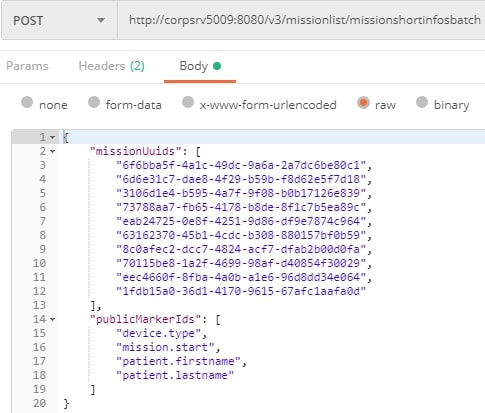
\includegraphics[width=.95\linewidth]{img/exRequestW}  
  \caption{Beispiel des POST-Requests}
  \label{fig:request}
\end{subfigure}
\begin{subfigure}{.5\linewidth}
  \centering
  % include second image
  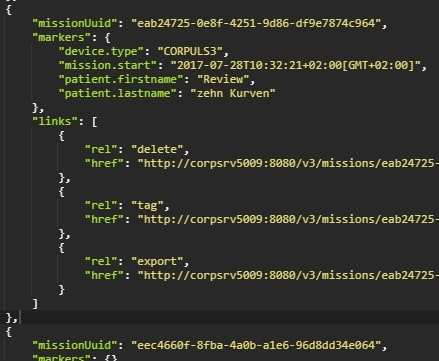
\includegraphics[width=.95\linewidth]{img/exResponse}  
  \caption{Auszug der Antwort auf den POST-Request}
  \label{fig:response}
\end{subfigure}
\caption[Beispiel einer Anfrage und Antwort der POST-Methode]{Beispiel einer Anfrage und Antwort der POST-Methode, um die \gls{MM} der im Body angegebenen Einsätze zu erhalten}
\label{fig:fig}
\end{figure}

In Abbildung \ref{fig:request} ist ein solcher POST-Request zu sehen.
In der URL wird der entsprechende \gls{ANALYSE}-Server adressiert, um auf die Daten der einzelnen Einsätze zugreifen zu können.
Im Body werden hierbei die aus Schritt 1 angeforderten Objekte eingefügt: \glqq missionUuids\grqq{} und \glqq publicMarkerIds\grqq.

Als Antwort erhält man mehrere \glqq Missions-Objekte\grqq{}, welche die \gls{UUID} und die entsprechenden \gls{MM} mit den individuellen Werten einer Mission enthält.
Ein Auszug einer solchen Antwort ist in \ref{fig:response} zu sehen.
Des Weiteren gibt es ein \glqq Link-Objekt\grqq{}, mit welchem ein Einsatz gelöscht, exportiert oder verändert werden kann. 

Positiv an diesem Export ist, dass die Anzahl der exportierten bedingt festgelegt werden kann.
Allerdings wird dieses Schema bei größeren Datenmengen, was genau das Ziel bei den Auswertungen ist, zu Problemen führen.
So kann das entsprechende Objekt mit den Einsatz-\gls{UUID}s sehr groß werden und beim kopieren und einfügen in den darauffolgenden Request-Body Schwierigkeiten bereiten.
Auch der damit resultierende große POST-Befehl ist keine optimale Umsetzung.

Aus diesem Anlass muss dieses Export-Format neu überdacht und für große Datenmengen optimiert werden.

\subsubsection{Überarbeitetes Export-Format}
\label{subsub:ueberarbeutetesformat}
Der Hauptaspekt beim neuen Entwurf der Export-Schnittstelle war das effiziente und sichere Umgehen mit großen Datenmengen.
Hierfür muss ein anderer als der zweistufige, in \ref{subsub:1stexport} beschriebene Prozess, entwickelt werden.

\todo{Alternativen: Direkt auf Platte, Anstoßen und direkt Ergebnis erhalten oder eben Anfrage und später fertige Datei\\
Warum letzteres: Nie Timeout und sicherheit(auth) und universell}
%\lipsum*[104]

Letztendlich wurde sich für ein/das Konzept mit den folgenden möglichen Schritten entschieden:
\begin{enumerate}
\item Die Generierung eines Exports anstoßen
\item Alle angeforderten Exports auflisten
	\begin{enumerate}
	\item Details zu einem explizitem Export bekommen
	\item Bestimmten Export löschen
	\end{enumerate}
\item Objekt/Datei mit allen Einsätzen und zugehörigen Daten mittels eigenem Link abrufen
\end{enumerate} 

Zum Erhalt der Export-Datei sind alle drei Schritte notwendig, 2a) \& b) sind als optionale Funktionen verfügbar.
Auch hier ist bei allen Vorgängen eine entsprechende Authentifizierung notwendig, um entsprechende Aktionen anzustoßen oder Informationen zu erhalten.

\begin{enumerate}
\item \code{-POST http://10.97.3.109:8080/v3/exports}
\end{enumerate}
Der erste Vorgang ist hierbei der POST-Befehl, der auf dem entsprechenden Server die Generierung eines neuen Exports anstößt.
Dabei werden alle verfügbaren Einsätze mit allen vorhandenen \gls{MM} exportiert.
Dies wurde so festgelegt, da der Anwender in der Regel mit einem solchen Export alle Missionen erhalten möchte.
Die Erweiterung um einen ressourcensparenden \glqq Incremental Load\grqq{} wird in \ref{sub:incremental} weiter betrachtet.

\begin{enumerate}[resume]
\item \code{-GET http://10.97.3.109:8080/v3/exports}
\end{enumerate}

Daraufhin ist es mit dem zweiten Schritt möglich, alle angestoßenen, laufenden und fertigen Exports aufzulisten.
Dabei wird mit der identischen URL die GET-Methode ausgeführt.
Hierbei werden pro Export zusätzliche Informationen bereitgestellt (siehe Abbildung \ref{fig:exportListWide}): 

%Die Start-Zeit (\glqq startTime\grqq) als UTC-Zeitstempel in Millisekunden, wann dieser Export angestoßen wurde.
%Analog der End-Zeitpunkt (\glqq endTime\grqq) wann dieser Export fertiggestellt wurde, die Anzahl Missionen, der jeweilige Status, ob angestoßen, laufend oder fertig, Links für weitere Optionen sowie die ID des Exports.

\begin{itemize}
\item Start-Zeit (\glqq startTime\grqq): UTC-Zeitstempel in ms, wann dieser Export angestoßen wurde
\item End-Zeit (\glqq endTime\grqq): UTC-Zeitstempel in ms, wann dieser Export fertiggestellt wurde
\item Anzahl der exportierten Einsätze (\glqq missions\grqq)
\item Status, ob angestoßen, laufend oder fertig
\item Links zu den weiteren Optionen
\item Die ID des Exports
\end{itemize}

\bild
{exportListWide}
{12cm}
{Antwort des Servers - Auszug der Auflistung von zwei fertiggestellten Exports als JSON-Objekte}
{Auflistung von Exports}

Demnach werden angeforderte Exports für eine ausgewählte Dauer gespeichert, was für unterschiedliche Szenarien ein Vorteil sein kann.
Auch die Möglichkeit, einen angeforderten Export wieder zu löschen ist eine hilfreiche Funktion, welche einen Server entlasten kann, sollten beispielsweise zu viele Exporte angefordert worden sein.
Der Status ist ebenfalls eine nützliche Information, welche den Empfang des fertigen Exports an ein \gls{BI}-Werkzeug erleichtern und garantieren kann.

\begin{enumerate}[resume]
\item \code{-GET http://10.97.3.109:8080/v3/exports/\{EXPORT\_ID\}/file}
\end{enumerate}

Im letzten Schritt wird der entsprechend bereitgestellte Link mitels GET-Methode aufgerufen.
Daraufhin erhält der Anwender den gesamten Export mit allen Einsätzen und den dazugehörigen \gls{MM} im JSON-Format. 
Ein Beispiel dieser Antwort ist Abbildung \ref{fig:exportFile} zu entnehmen.
\bild
{exportFile}
{9cm}
{Auszug des Exports mit allen Einsätzen und dazugehörige \gls{MM}}
{Auszug des Exports}

Der größte Vorteil dieses neuen Formats ist der Umgang mit großen Datenmengen.
Es müssen keine riesigen Objekte kopiert und eingefügt oder an eine andere Stelle weitergeleitet werden. 
Auch sind keine weiteren umständlichen Parameter notwendig. \\
Die URL wurde mit dem Schema \\
\colorbox[RGB]{240,240,240}{\texttt{http://\{SERVER\_IP\}/v3/exports}} \\
standardisiert, sodass keine unterschiedlichen URLs mit vielen optionalen Parametern wie in \ref{subsub:1stexport} notwendig sind.
Lediglich beim finalen Anfordern der Export-Datei muss die Standard-URL um \\
\colorbox[RGB]{240,240,240}{\texttt{http://\{SERVER\_IP\}/v3/exports\textcolor{red}{/\{EXPORT\_ID\}/file}}} \\
erweitert werden. 

\subsection{Erweiterung um neue Datenobjekte} %tiefgreifendere? Daten}
\label{sub:erweiterung}
Im Rahmen der \fullref{kap:anforderungsanalyse} kamen bereits erste Fragestellungen zum Vorschein, welche mit den bisherig zur Verfügung stehenden Daten nicht beantwortbar waren.
Im darauffolgenden Laufe der \fullref{kap:konzept} haben sich diverse weitere Problematiken und fehlende Daten für aussagekräftige Auswertungen bestätigt.

So ist beispielsweise eine ausdrucksvolle Analyse zur Drucktiefe in der Reanimation über mehrere Missionen nicht in der Form umsetzbar, wie sie sinnvoll und gewünscht wäre.
Hier ist lediglich der Mittelwert der Drucktiefe von der gesamten Reanimation vorhanden.
Eine inhaltsreiche Auswertung, auch beispielsweise mit Veränderungen innerhalb der Reanimation, sind schlicht nicht möglich.
In diesem Stil gibt es weitere, für Auswertungen sinnvolle Daten, die derzeit gar nicht, oder nur als stark aggregierte Werte vorhanden sind.
Eine Analyse der potentiell verfügbaren Daten ergab folgende Bereiche (Auszug im Anhang \ref{anhangProbleme}):  %Markante Beispiele sind:
\begin{description}
\item [Reanimationsqualität]\hfill \\
Drucktiefe \& -frequenz, Anzahl Kompressionen, Pausenzeiten und \gls{CCF}
\item [Defibrillationen]\hfill \\
Zeitpunkt, Energie, Impedanz, Modus und Pausenzeiten der einzelnen Defibrillationen
\item [\gls{NIBD}]\hfill \\
Zeitpunkt, Modus, Dauer , Patiententyp, Systole, Diastole \& mittlerer arterieller Druck der einzelnen Messungen
\item [Vitalparameter und Trends]\hfill \\
Die Werte aller Vitalparameter zu einem bestimmten Zeitpunkt
\item [Technische- und Patienten-Alarme]\hfill \\
Wann sind welche Patientenalarme mit welchen Alarmgrenzen aufgetreten? \\
Welche technischen Alarme treten zu welcher Zeit auf?
\item [Events]\hfill \\
Welche Events treten wann mit welchen Parameter-Werten auf?
\end{description}

Mit diesen Daten wären weit detailliertere und tiefgreifendere Auswertungen möglich. 
Dabei würde vor allem die explorative Datenanalyse (siehe S.\pageref{subsub:datenanalyse}, \ref{subsub:datenanalyse}) profitieren.

Diese erfordern jedoch eine Überlegung des späteren Datenmodells, da diese das Konzept von multidimensionale Daten darstellen.
Demnach gibt es einen Datensatz mit \textit{n} Einsätzen, wovon jeder Einsatz eine Anzahl \textit{m} Kompressionen, Defibrillationen, Messungen, Alarme und weiteres haben kann.
Einen Entwurf für ein passendes Datenmodell ist in Abbildung \ref{fig:ersterVorschlagDatenmodellC} zu sehen.

Auf Basis dieser Analyse und der herausgefundenen potentiellen neuen Datenquellen werden Anforderungen formuliert und mit der Entwicklungsabteilung kommuniziert, damit diese Daten zur Auswertung bereitstehen können.

\subsubsection{Entwurf für ein Datenmodell}
\label{subsub:datenmodell}
Um die Anforderung, weitere Daten aus den bisherigen Einsätzen auszulesen gerecht zu werden, muss vorab ein geeignetes Datenmodell entworfen werden.
Dieses muss die daraus resultierende Multidimensionalität unterstützen und eine konfliktfreie Umgebung schaffen.
Dabei sollen jedoch so viele Daten wie möglich miteinander kombiniert werden können, damit ein umfassendes exploratives und konfirmatives Analysieren der vorliegenden Daten möglich ist.

Zuvor gab es lediglich die Tabelle \glqq Missions\grqq{}, welche pro Zeile einen Einsatz ablegt und in den dazugehörigen Spalten die Werte zu den entsprechenden \gls{MM}.
Ein Auszug aus hieraus ist in Tabelle \ref{tbl:missions} zu sehen.

\begin{table}[htb]
\centering
%\resizebox{\textwidth}{!}{%
\begin{tabular}{|l|l|l|l|l|}
\hline
\textbf{mission.uuid}   & \textbf{mission.start} & \textbf{hasReanimation} & \textbf{device.type} & \textbf{...} \\ \hline
b14f790f-{[}...{]}863f3 & 2016-08-27T12:13:07    & true                    & corpuls3             & ...          \\ \hline
d7276b88-{[}...{]}2da61 & 2016-09-29T21:02:30    & false                   & corpuls1             & ...          \\ \hline
\end{tabular}%
%}
\caption[Aktuelle Export-Tabelle]{Auszug aus der Tabelle, wie sie im aktuellen Export maximal zur Verfügung steht}
\label{tbl:missions}
\end{table}

Ein geeignetes Datenmodell, welches die mehrdimensionalen Daten einbindet und unterstützt, wurde entworfen und ist in Abbildung \ref{fig:ersterVorschlagDatenmodellC} zu erkennen.
Hierbei wurden die in \ref{sub:erweiterung} genannten neuen Datenquellen hinzugefügt, sodass beispielsweise neue Tabellen zu \gls{CPR}- oder Defibrillationsdaten zu sehen sind.

\bildbreit
{ersterVorschlagDatenmodellC}
{Visualisierung für den Entwurf eines neuen Datenmodells mit mehrdimensionalen Objekten}
{Visualisierung des neuen Datenmodells mit mehrdimensionalen Objekten}

Dabei wurde darauf geachtet, dass keine zirkulären Referenzen entstehen, welche unter anderem bei der gleichen Benennung mehrerer Spalten vorkommen.
Dies wurde präventiv mit einem Präfix der jeweiligen Datenquelle verhindert.
Auch erleichtert dies das spätere Erstellen von Dimensionen oder Kennzahlen, da eine eindeutige Benennung vorhanden ist.

Auch ein gemeinsamer Primärschlüssel sollte in allen neuen Datentabellen vorhanden sein, damit eine Beziehung herrscht.
Hierfür wurde die \gls{UUID} verwendet, da diese garantiert in jedem Einsatz vorhanden und bereits eindeutig ist.
Damit ist gewährleistet, dass theoretisch jeder Datenpunkt mit jedem anderen Datenpunkt verknüpft werden kann, auch wenn nur ein geringer Teil aller Verknüpfungen sich als sinnvoll erweisen wird. 


%\subsection{Incremental Load?}
\subsubsection{Erstellen von Anforderungen für neue Datenquellen} %(als User Stories in JIRA)}
\label{subsub:stories}
Damit die im vorherigen Kapitel herausgefundenen Datenquellen für Auswertungen bereitstehen, muss zunächst deren Extrahierung aus den Einsatzdaten implementiert werden. 
Weiter steht der Export, beziehungsweise das Hinzufügen dieser neuen Daten in den bestehenden, überarbeiteten Export an.

Hierfür wird der bestehende Prozess der Entwicklungsabteilung angewandt, damit eine entsprechende Implementierung im SCRUM-Verfahren möglich ist.
Demnach wird für eine neue Anforderung eine \glqq Story\grqq{} im Projekt- und Aufgabenmanagement-Tool \glqq Jira\grqq{} angelegt.
Diese Story wird einem übergeordneten \gls{Feature} oder \glqq Epic\grqq{} zugeordnet.
So werden beispielsweise dem Feature \glqq \gls{BI} Dashboard\grqq{} alle zugehörigen Storys zugeordnet, wie in einem Auszug davon in Abbildung \ref{fig:jiraEpic} zu sehen ist.
\bild
{jiraEpic}
{12cm}
{Grafische Visualisierung der zugehörigen Storys vom Feature \glqq \gls{BI} Dashboard\grqq{} in Jira}
{Visualisierung der zugehörigen Storys vom Feature BI-Dashboard in Jira}

Weiter muss eine Story laut SCRUM die \glqq Definition of Ready\grqq{} erfüllen, damit sie in den Sprint mit eingeplant werden darf.
Diese soll garantieren, dass unter anderem eine aussagekräftige Beschreibung oder Abnahmekriterien vorhanden sind.
Dementsprechend müssen die erstellten Storys gewisse Qualitätsmerkmale vorweisen, damit sie umgesetzt werden können.

Für das Extrahieren und Exportieren von einem neuen Datenobjekt ist es daher sinnvoll, die geforderten Informationen so detailliert wie möglich darzulegen.
Hierfür ist das vorab in \ref{subsub:datenmodell} entwickelte Datenmodell ein hilfreiches Mittel, um die Storys präzise beschreiben zu können.

\begin{table}[hbt]
\centering
\resizebox{\textwidth}{!}{%
\begin{tabular}{ll|l|l|l|l|l|l|}
\cline{3-8}
                                       &                       & \multicolumn{6}{c|}{\textbf{trend.}}                                                                                                                                              \\ \cline{3-8} 
                                       &                       &                       & \multicolumn{5}{c|}{\textbf{cpr.}}                                                                                                                        \\ \hline
\multicolumn{1}{|l|}{\textbf{}}        & \textbf{mission.uuid} & \textbf{minute} & \textbf{pauses.sum} & \textbf{comp.sum} & \textbf{depth.avg} & \textbf{rate.avg} & \textbf{ccf} \\ \hline
\multicolumn{1}{|l|}{\textbf{Type}}    & uuid                  &                       & int                           & int                                 & float                        & float                       & float                  \\ \hline
\multicolumn{1}{|l|}{\textbf{Unit}}    &                       &                       & s                             &                                     & cm                           & 1/min                       &                        \\ \hline
\multicolumn{1}{|l|}{\textbf{Example}} & sd84-[...]-k9s4s      & 3                     & 13                            & 91                                  & 5.31                         & 112                         & 0.82                   \\ \hline
\end{tabular}%
}
\caption[Gefordertes Exportformat am Beispiel der CPR-Daten]{Auf Basis des entworfenen Datenmodells erstellte Tabelle für das geforderte Export-Format am Beispiel von \gls{CPR}-Daten}
\label{tbl:export}
\end{table}

Für eine solche detaillierte Beschreibung der Story wurde unter anderem eine Tabelle \ref{tbl:export} angelegt.
In dieser Darstellung sind bereits viele Aspekte festgelegt.
So ist beispielsweise die Namensgebung an die bisherige Nomenklatur der \gls{MM} angelehnt, sodass eine innere Konsistenz herrscht.
Auch der jeweilige Datentyp oder die Einheit ist bereits festgelegt, damit ein einheitliches Format der Daten gewährleistet ist.

Die Einheit ist insofern von großer Bedeutung, da diverse Daten in verschiedenen Einheiten gespeichert werden können.
So kann etwa die CO2-Konzentration der Ausatemluft in Millimeter-Quecksilbersäule (mmHg) oder Kilopascal (kPa) gemessen und gespeichert werden.
Damit in der späteren Auswertung keine unterschiedlichen Einheiten vermischt werden, wird in Tabelle \ref{tbl:export} eine Standard-Einheit für den Export festgelegt.

Auch der Aggregierungsgrad wird hier beschrieben, indem die Daten für eine Minute aggregiert werden sollen.
Dies resultierte aus mehreren Diskussionen mit Entwicklern, Produktmanager und Stakeholdern, da die Speicherung von jeder einzelnen Kompression mit ihren vorliegenden Daten auf lange Sicht zu einem Speicher- und Performanceproblem führen könnte.
Dennoch ist es für die Anwender eine deutliche Verbesserung der Auswertungsmöglichkeiten.

Ein Beispiel für exemplarische Daten wird ebenfalls hinzugefügt, damit letzte Unklarheiten zu Feldern oder Datentypen beseitigt werden.
Dieser Prozess wird analog mit allen neu geforderten Objekten (siehe Abbildung \ref{fig:ersterVorschlagDatenmodellC}) durchgeführt. Anhang\ref{AnhangJiraStories?}

\subsubsection{Festlegen des Export-Formats}
Im Zuge der Bereitstellung der neuen Datenobjekte wurde im vorigen Kapitel mittels Beschreibung der Anforderungen und ergänzenden Tabellen das gewünschte Format festgelegt.
Im Laufe der Implementierung gibt es diverse Diskussionen und Abstimmungen mit den Entwicklern und Stakeholdern, wie der finale Export aussehen soll.
Dies geschieht im Zuge der \glqq Sprints\grqq{} in mehreren Zyklen, wird jedoch für die bessere Lesbarkeit dieser Arbeit in diesem Unterkapitel zusammengefasst.

Vorab ist anzumerken, dass im zeitlichen Rahmen dieser Arbeit und unter Berücksichtigung von anderen Entwicklungsprojekten eine Priorisierung des Product-Owners vorgenommen werden musste.
Dabei sind drei der sechs geforderten neuen Datenobjekte aus Abbildung \ref{fig:ersterVorschlagDatenmodellC} für die Erweiterung des Exports  geplant: \gls{CPR}-, \gls{NIBD}- \& Defibrillations-Daten.

Demnach soll es drei optionale neue JSON-Objekte in der Antwort des Servers (siehe Abbildung \ref{fig:exportFile}) geben.
Hier wurden vorab Überlegungen getätigt, wo die entsprechenden neuen Daten hierarchisch zugeordnet werden.
Dabei gibt es generell zwei Optionen:
Die neuen Objekte dem \glqq markers\grqq-Objekt unterordnen (Abbildung \ref{fig:marker}), oder direkt unterhalb des \glqq mission\grqq-Objektes als zweiten Kindknoten (\ref{fig:mission}).

\begin{figure}[ht]
\begin{subfigure}{.5\linewidth}
  \centering
  % include first image
  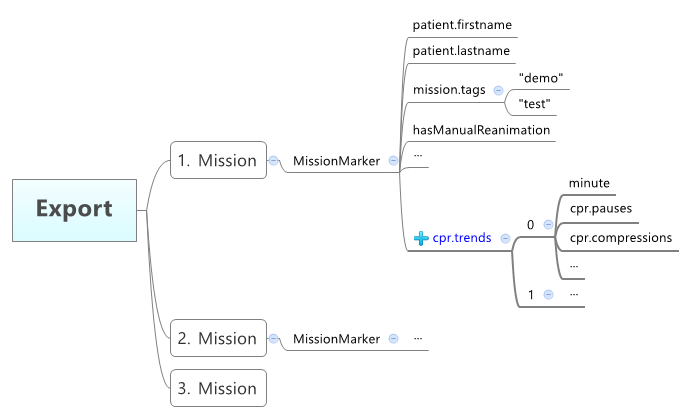
\includegraphics[width=.95\linewidth]{img/format1}  
  \caption{CPR-Objekt unterhalb des \glqq markers\grqq-Objekt}
  \label{fig:marker}
\end{subfigure}
\begin{subfigure}{.5\linewidth}
  \centering
  % include second image
  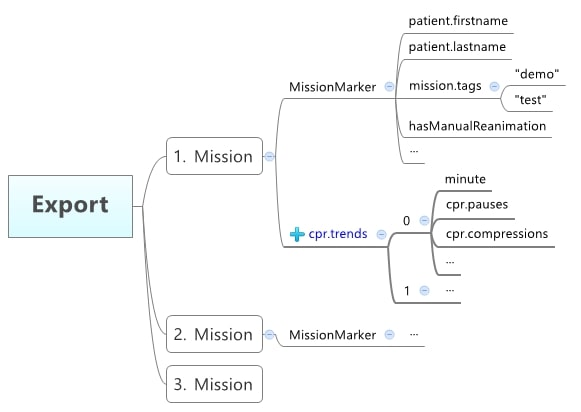
\includegraphics[width=.95\linewidth]{img/format2}  
  \caption{Neues Objekt neben dem \glqq markers\grqq-Objekt}
  \label{fig:mission}
\end{subfigure}
\caption[Beispiel einer Anfrage und Antwort der POST-Methode]{Schematische Darstellung der Erweiterung des Exports am Beispiel vom CPR-Objekt}
\label{fig:tree}
\end{figure}

Da es sich um eigenständige neue Objekte unabhängig von den \gls{MM} handelt, wurde sich für die Variante in Abbildung \ref{fig:mission} entschieden.
Demnach können nun die Objekte \glqq trend.cpr\grqq, \glqq shock.details\grqq{} und \glqq nibp.details\grqq{} in einem Missions-Objekt vorhanden sein.
Ein Beispiel hierfür ist in Abbildung \ref{fig:exportNewObj} zu sehen.

\bild
{exportNewObj}
{9cm}
{Neue JSON-Objekte (hier \glqq trend.cpr\grqq{} \& \glqq shock.details\grqq{}) neben den \glqq markes\grqq{} innerhalb eines Missions-Objektes des Exports}
{Neue JSON-Objekte innerhalb eines Missions-Objektes des Exports}

%(Diese zwei Optionen sind in Abbildung \ref{fig:tree} schematisch dargestellt.
%Dabei ist in \ref{fig:marker} das Schema mit der Unterordnung unterhalb des \glqq markers\grqq-Objekt visualisiert.
%In \ref{fig:mission} ist das \gls{CPR}-Objekt unterhalb der ersten Mission als zweites Kindobjekt neben den \glqq markers\grqq angelegt.)

Des Weiteren wurde entschieden, die neuen Objekte nur zu exportieren, wenn auch tatsächlich Daten hiervon vorhanden sind.
Bei dem \gls{CPR}-Objekt gibt es hierbei eine Besonderheit, da dieses als zeitliches Objekt mit Trenddaten anzusehen ist.
Dadurch gibt es immer Daten ab Minute 0, auch wenn beispielsweise die erste Kompression erst in Minute zwölf stattfand.
Dies soll garantieren, dass eine kontinuierliche Zeitskala gegeben ist, die auch mit anderen Trenddaten vergleichbar ist.
Für eine Vergleichbarkeit von Reanimationen untereinander ist diese Form der Daten nicht geeignet. 
In \ref{subsub:weitereFelder} wird eine Lösung erarbeitet, die dies zusätzlich ermöglichen soll.

Bei den \gls{NIBD}- \& Defibrillations-Objekten ist im Gegensatz zum CPR-Objekt nicht die Minute das führende Feld respektive Primärschlüssel, sondern die hochzählende Nummer der Messung oder der Schockabgabe.
Dadurch ist aufgrund der Objekorientierung eine Repräsentation der Wirklichkeit gegeben, da eine Messung oder eine Defibrillation ein abgeschlossenes Objekt darstellt.

%(json format cpr (siehe mails) (Fotos whiteboard als anhang?),)
%null values bei cpr trends

%% Vor Export?
%\subsection{Datenbankhaltung?}
%\subsubsection{Lasttests?}
%%dummydaten?


%\section{Datenmodell?}

\section{Erstellung der Qlik-App(s)}
\label{sec:erstellung}
%subsUnterschiedliche Apps?
\subsection{ETL-Prozess}
\label{sub:etl}

\subsubsection{Ladeskripte}
\label{subsub:scripts}

\subsubsection{Demo- und Testeinsätze herausfiltern}
\label{subsub:testfilter}

\subsubsection{Weitere manuell hinzugefügte Felder (ReaStart, Calendar, Test...)}
\label{subsub:weitereFelder}


\subsection{Datenmodell (hier oder eigene section?)}
\label{sub:datenmodell}

\subsection{Dimensionen}
\subsection{Kennzahlen}
\subsection{Verwendung von Erweiterungen?}
\subsection{Dashboards}
\subsubsection{Neue mögliche Visualisierungen durch Anforderungen Schocks, Nibp, Cpr}
test
\subsection{Umsetzung der Evaluierungsergebnisse (Auszug)}
\subsubsection{Zielgruppenunterschiedliche Startseiten}
\subsubsection{Lesezeichen?} %vlt so 10 Beispiel Lesezeichen
\subsubsection{Usability/Nutzerführung/Hilfetexte}
\subsubsection{Reduzierung Inhalt pro Arbeitsblatt}
\subsubsection{Weitere}
%subs testeinsätze filtern

\subsection{Einstellungen der Arbeitsblätter und Diagramme}
% (wie zB. Farben bei Auswahl beibehalten)
%CustomThemes?
%subs internationalisierung

% Aspekte vor Erstellung??
\section{Rechtliche Aspekte?}
\subsection{Datenschutz}
\subsection{Anonymisierung}


\section{Sonstige Aspekte?}
\subsection{Auslieferungsprozess?}
\subsection{Internationalisierung}
\subsection{Incremental Load?}
\label{sub:incremental}


\section{Evaluierung der Ergebnisse?}
%subs Usability-Tests?

\chapter{Diskussion}
\label{fazit}
\minitoc\pagebreak

\section{Fazit}
Ziel dieser Arbeit war die Bearbeitung der zugrundeliegenden Fragestellungen (\ref{fragen}).
Demnach sollten Anforderungen respektive Fragen der Nutzergruppen gesammelt und auf benötigte Daten analysiert werden.
Aus diesen Erkenntnissen resultiert die Modellierung eines geeigneten Datenmodells und auf Basis dieses Modells sollten entsprechend aussagekräftige Dashboards entwickelt werden.

Es wurden diverse Interviews mit vielen repräsentativen Personen geführt, um ein Bild der im Raum stehenden Fragen zu erhalten.
Dabei lag der Schwerpunkt auf interne Mitarbeiter, welche aufgrund des häufigen Hintergrundes im Rettungsdienst oder Kontakt zu diesem durchaus eine gefestigte Gruppe mit einer repräsentativen Meinung darstellen.
Es konnte auch ein Treffen zu dieser Thematik mit einem tatsächlichen Kunden der Nutzergruppe \glqq Ärztlicher Leiter Rettungsdienst\grqq{} arrangiert werden, aus welchem die Erkenntnisse mit besonderer Gewichtung in die weitere Entwicklung eingeflossen sind.
Hierbei wurde anfangs die Methodik der Einzelinterviews angewandt, welche sich retrospektiv als positiv erwiesen hat, da die unvoreingenommene Meinung der Einzelpersonen dadurch abgefragt werden konnte.
So entstand ein großes Sammelwerk an Anforderungen, welche in dieser Arbeit die Form von Fragestellungen haben (Auszug im Anhang \ref{att:anforderung}).
Diese wurden in zyklisch-iterativen Vorgängen später weiter analysiert und spezifiziert, so wie es die Prozesse des Requirements Engineering vorsehen \cite{ Bergsmann.2018, Leffingwell.2011, Patig., Pohl.2011}. 
Dabei wurden auch Gruppendiskussionen angesetzt, um ein kollaboratives Evaluieren und eine Auseinandersetzung mit anderen Meinungen zu ermöglichen.

Parallel wurden erste konzeptionelle Prototypen von Diagrammen entwickelt, um herauszufinden, welche Fragen bereits beantwortet werden können.
Auch erste Rückschlüsse für ein Datenmodell konnten hierbei extrahiert werden.
Dabei wurden verschiedene Modelle anhand von methodischen Schemata und Architekturen aus Literatur (\cite{Bauer.2004, Gabriel.2011, Gitelman.2013, Kimball.2013, Mucksch.2000}) herangezogen und mit den vorliegenden Daten untersucht.
Diese Prototypen wurden wiederum mit den entsprechend befähigten Mitarbeitern der Firma evaluiert, sodass auch hier etwaige Kritik berücksichtigt und schnell darauf reagiert werden kann.

Anhand der Ergebnisse dieser Untersuchungen konnten tatsächliche Anforderungen an die Software \gls{ANALYSE} gestellt werden, ob neue Daten aus den Einsätzen zur Verfügung gestellt werden müssen.
Auch die Spezifikation, in welchem Format die Daten benötigt werden (Anhang \ref{att:stories}), sowie das bestmögliche Export-Format (\ref{sub:export}) waren Bestandteil dieser Arbeit. 

Da all diese Prozesse mehr oder minder parallel abliefen, ist eine strikte Trennung nicht möglich.
Es wurden stets neue Fragen erhoben, bestehende analysiert und spezifiziert und währenddessen wurde an dem Datenmodell, Prototyp oder der letztendlichen Umsetzung der Qlik-App gearbeitet.
Dabei wurden auch immerzu diverse Richtlinien, Usability-Erkenntnisse und Grundsätze zur Visualisierung von Daten und Gestaltung von Dashboards (\cite{Bassler.2010, Card.2007, Fischer.2014, FischerStabel.2018, Hichert.2017, Kertzel.2018, Mccormick.1987, Schumann.2000, Ware.2009}) berücksichtigt, um möglichst konflikt-freie und ansprechende Auswertungen für die Anwender zu ermöglichen.
Die endgültigen, in dieser Arbeit entstandenen Dashboards können dem Anhang \ref{att:dashboards} entnommen werden.

\todotext{see comment}

%\section{Vorstellung der Ergebnisse}

%\section{Rückschlüsse für weitere Entwicklung}
%
%\subsection{Rechtliche Aspekte?}
%\label{sub:recht}
%
%%anonymisierung, datenschutz 
%
%%\subsubsection{Datenschutz}
%%\subsubsection{Anonymisierung}
%
%%als sub hier rein?
%\subsection{Sonstige Aspekte?}
%
%\subsubsection{Incremental Load?}
%\label{sub:incremental}
%\subsubsection{Internationalisierung}
%\subsubsection{Auslieferungsprozess?}
%
%
%% Aspekte vor Erstellung??
%
%
%%\section{Aufgetretene Probleme?}
%
%%\section{Erfüllte Anforderungen}
%%\subsection{Nutzeranforderungen}
%%\subsection{Theoriebasierte Anforderungen}

\section{Ausblick}
Die Arbeit hat einen Grundstein gelegt, um aus den zuvor nicht genutzten Daten einen Mehrwert zu erhalten.
Ein Export von relevanten Daten in einem geeigneten Format und die erste Überführung in ein effizientes Datenmodell waren die ersten Schritte in der Richtung \glqq Big Data Analytics\grqq {}.

Da Big Data laut Literatur \cite{Fischer.2014, Hausler.2018} in der Regel unstrukturierte Daten sind, und die für diese Dashboards zugrundeliegende Daten größtenteils strukturiert sind, ist es zum jetzigen Zeitpunkt kein handfestes \glqq Big Data Analytics\grqq{} (siehe  S. \pageref{fig:interrelations}, Abbildung \ref{fig:interrelations}).
Dennoch ist es ein erster Schritt in die entsprechende Richtung und kann in Zukunft weiter ausgeführt werden.

Es ist ein Reporting nach \gls{BI}-Praktiken entstanden, welches Daten aus unmittelbarer Vergangenheit\footnote{Nach Upload einer Mission auf den \gls{ANALYSE}-Server ist eine Aktualisierung der Visualisierungen binnen 5-10 Sekunden möglich (Bei einem Datenbestand von $\approx$ 10.000 Einsätzen; ungefähr linear skalierend)} in den erarbeiteten Dashboards anzeigt.
Bei dem späteren produktiven Einsatz bei Kunden wird es auch die professionelle Variante geben mit der Möglichkeit des Self-Service-Reporting.
Hierbei können die Anwender, statt der vorgefertigten Dashboards, eigene Diagramme und Dashboards auf Basis des hier erarbeiteten Datenmodells und \gls{DWH} zusammenstellen.

In Zukunft ist es denkbar, neue Technologien, Methodiken und Ansätze des Bereichs \glqq Data Analytics\grqq{} anzuwenden.
Spannend ist hierbei vor allem der Bereich \glqq Artificial Intelligence\grqq{} (AI) beziehungsweise künstliche Intelligenz (KI).
Mit Algorithmen wie \glqq Machine Learning\grqq{} oder \glqq Deep Learning\grqq{} sind gänzlich neue Einblicke, Erkenntnisse Trends oder gar Vorhersagen möglich.

Die Basis durch die nun exportierbaren Daten in einem adäquaten Format ist gelegt.
Die theoretischen Algorithmen und entsprechende Bibliotheken zum Programmieren werden immer ausgereifter und bilden so im Einklang mit den technischen und medizinischen Daten die besten Voraussetzungen, bisher unentdeckte Erkenntnisse zu gewinnen, die möglicherweise schon bald viele Leben retten könnten.


%\subsection{Mehrwert}


%%%%%%%%%% ENDE KAPITEL
\pagenumbering{Roman} % römische Ziffern für die Anhänge

\begin{appendix}
% Glossar
%\setglossarysection{section}
%\glsaddall
\setglossarysection{chapter}
\printglossary[numberedsection,style=altlist,title=Begriffsdefinitionen]
\label{chap:Definitionen}

\chapter{Anforderungsermittlung}
\section{Persona}


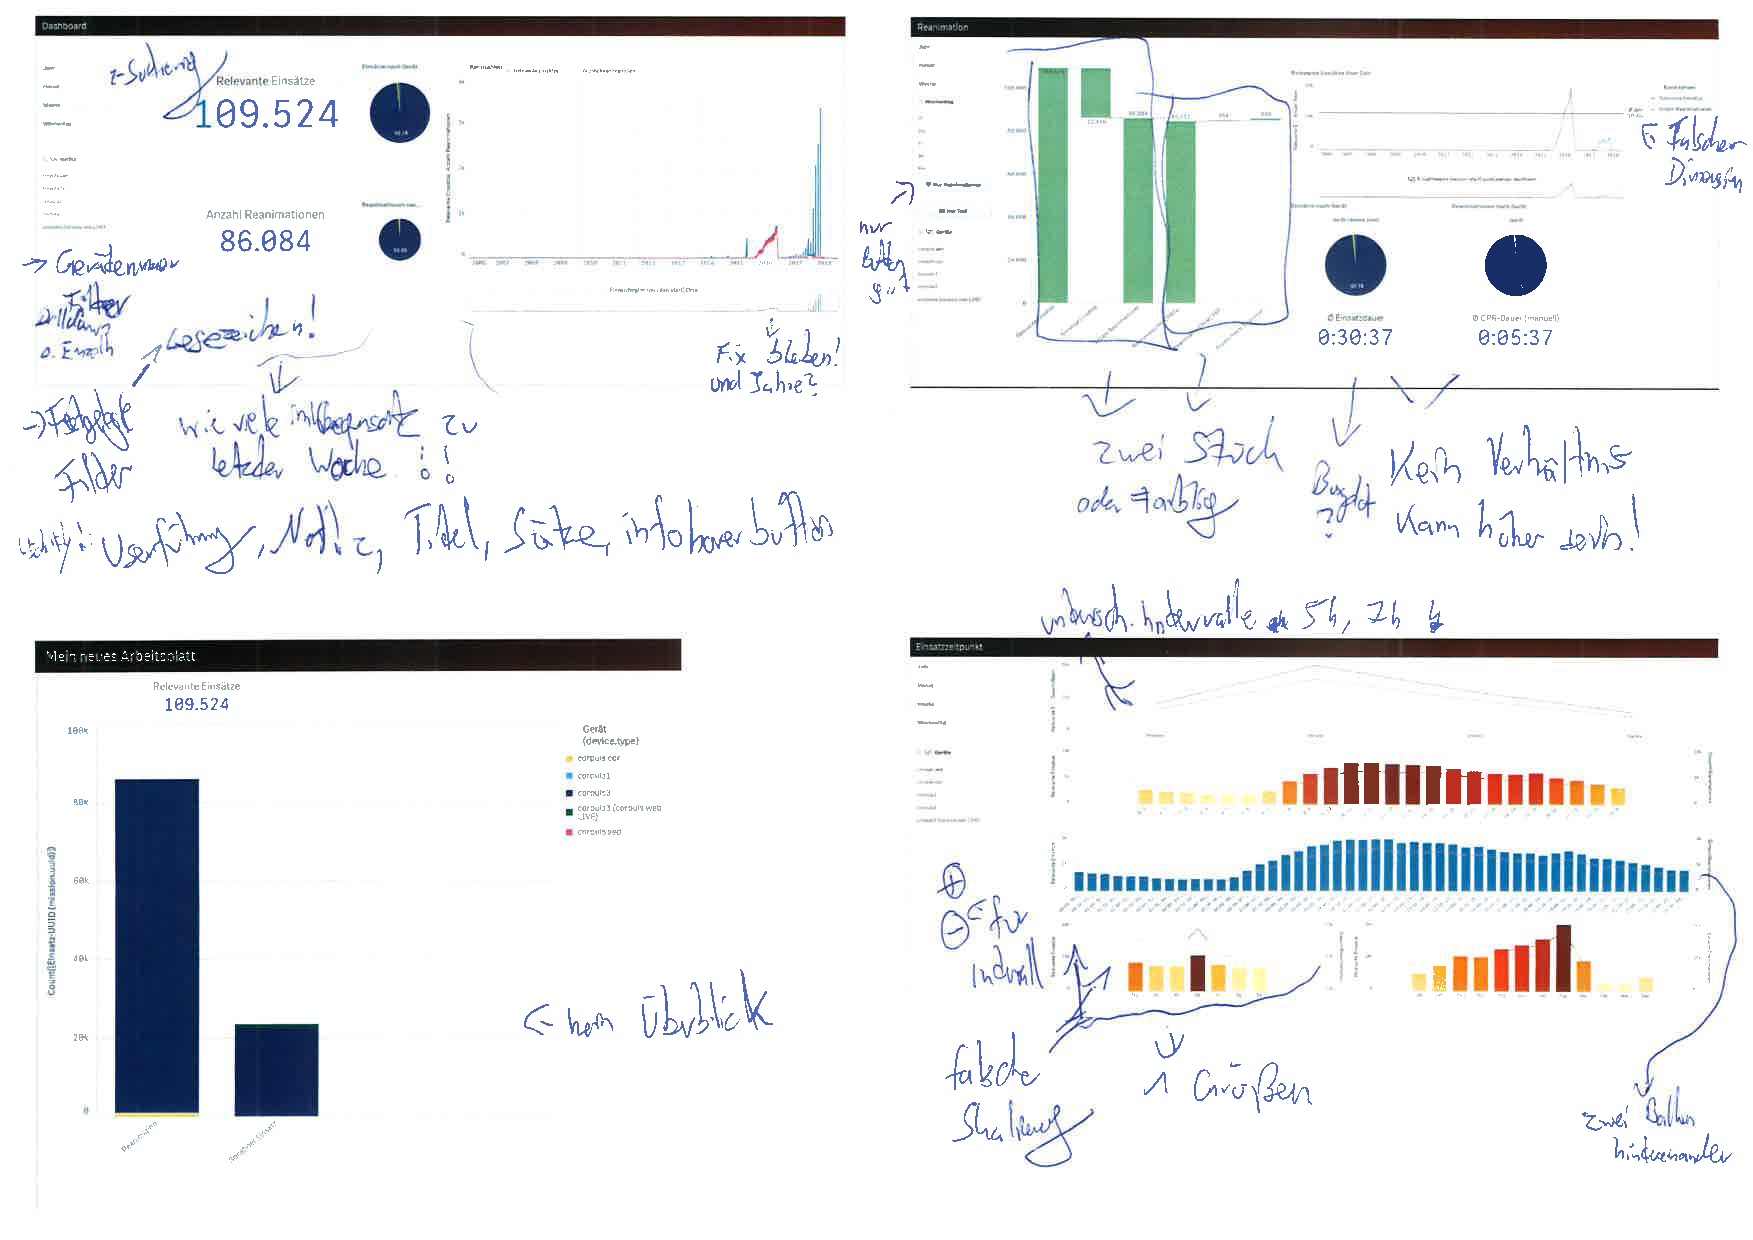
\includepdf[pages=1-2, nup=1x2, scale=0.7, pagecommand=\chapter{Evaluation}\label{att:evaluation}, offset=0 -2cm]{attachments/ALL_EVALUATION2.pdf}
%\includepdf[pages=3, nup=1x2, scale=0.7]{attachments/ALL_EVALUATION2.pdf}
\includepdf[pages=4-15, nup=2x2, scale=0.8,  pagecommand=\thispagestyle{headings}]{attachments/ALL_EVALUATION2.pdf}
\includepdf[pages={3, 16-22}, nup=1x2, scale=0.8, pagecommand=\thispagestyle{headings}]{attachments/ALL_EVALUATION2.pdf}

%\chapter{Dashboards}
%\includepdf[pages=-, nup=1x2, scale=0.6, landscape=true]{attachments/d12.pdf}

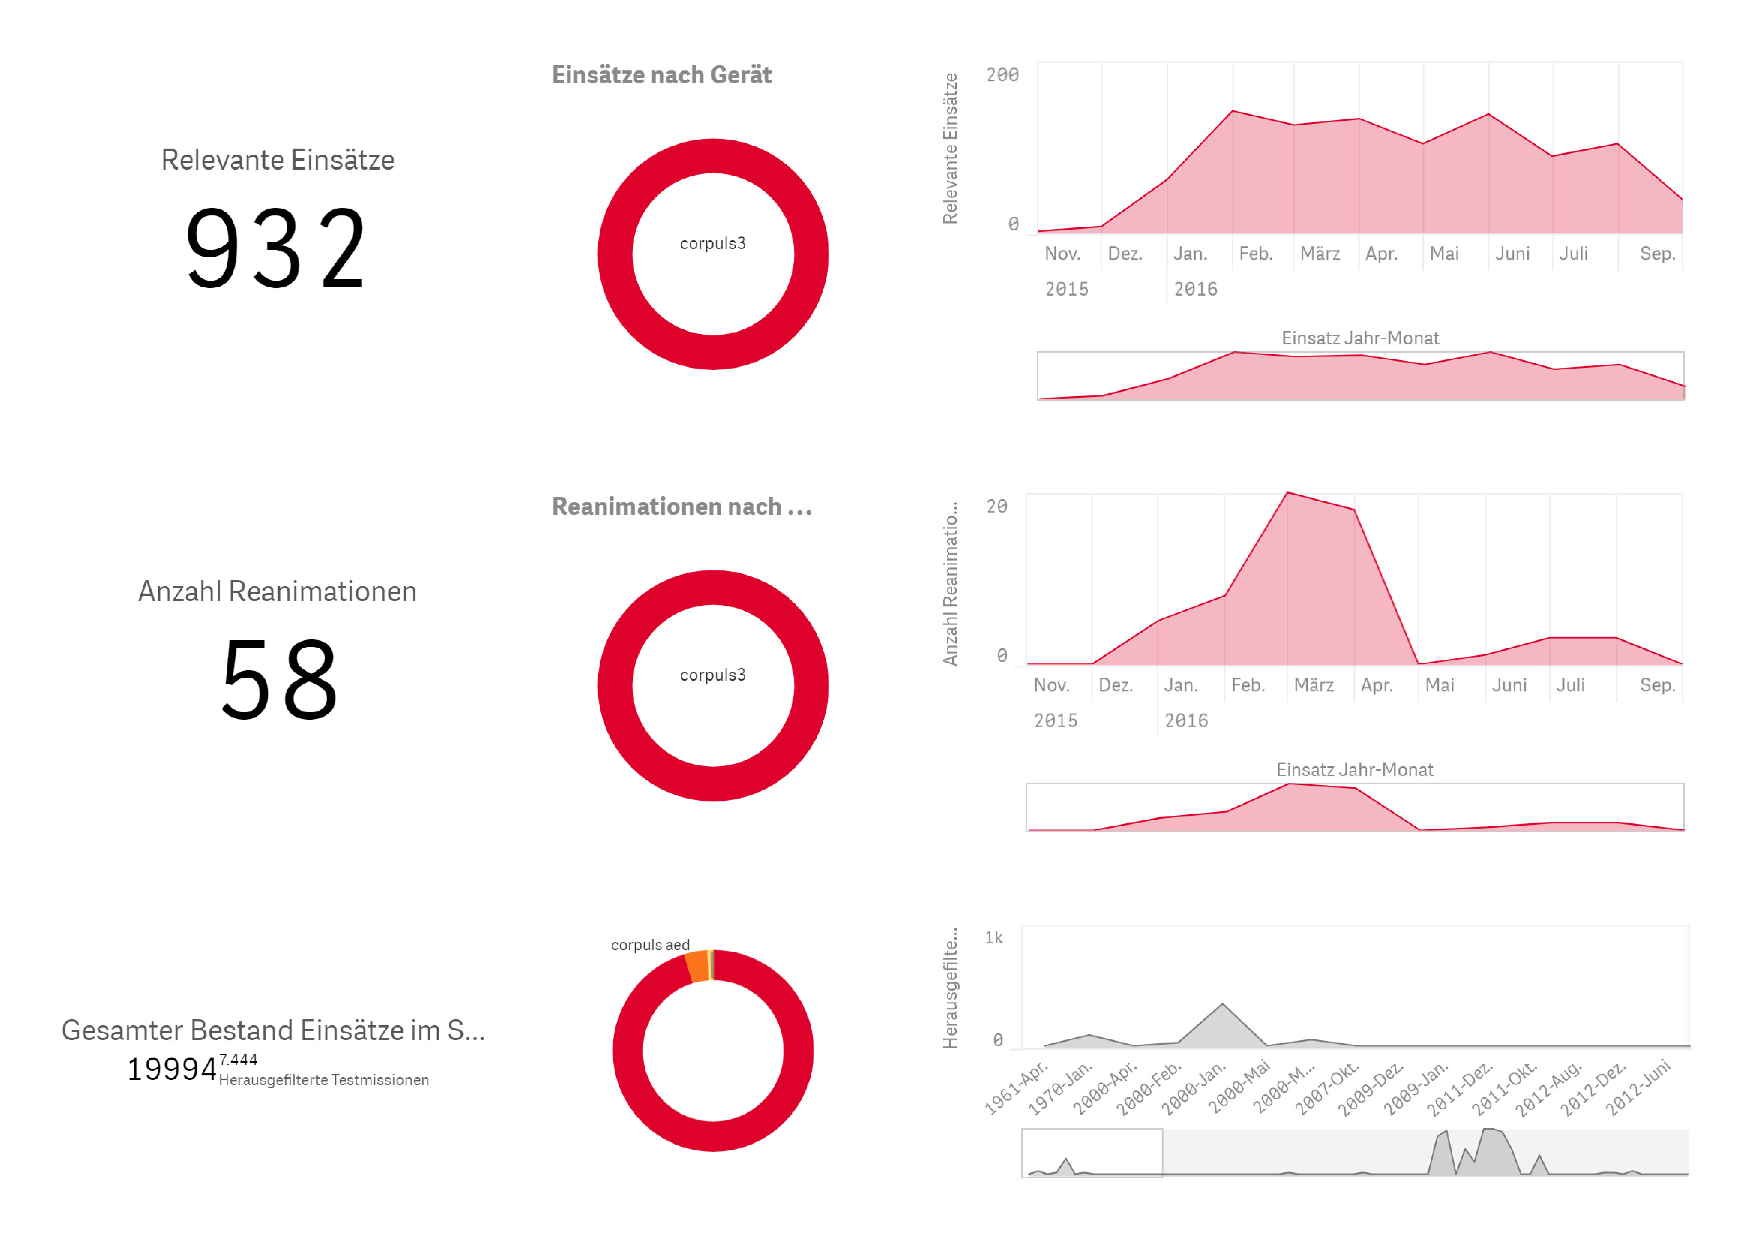
\includepdf[pages=-, nup=1x2, scale=0.7, pagecommand=\chapter{Dashboards}\label{att:dashboards}, offset=0 -2cm]{attachments/d12A1b.pdf}

\chapter{JSON Custom Theme}

\end{appendix}

%%%%% Verzeichnisse (Literatur, Abkürzungen, etc)
\singlespacing
% VERZEICHNISSE

%%%% BEGINN VERZEICHNISSE

% Abkürzungen 
\deftranslation[to=German]{Acronyms}{Abkürzungsverzeichnis}
\printglossary[type=\acronymtype,style=long]

% Abbildungsverzeichnis
\listoffigures

% Tabellenverzeichnis
\listoftables

% Bibliographie
\nocite{*} % Diese Zeile löschen, wenn nur verwendete Literaturangaben auftauchen sollen
\bibliographystyle{abbrvdin}
\bibliography{bibliographie}

%%%% ENDE VERZEICHNISSE
\onehalfspacing

%%%% Danksagungen
\newpage
\chapter*{Danksagung}
\thispagestyle{empty}

dank

%%%%% Eidesstattliche Erklärung
\newpage
\chapter*{Eidesstattliche Erklärung}
\thispagestyle{empty}
Ich erkläre hiermit an Eides statt, dass ich die vorliegende Arbeit selbstständig und ohne Benutzung anderer als der angegebenen Hilfsmittel angefertigt habe.
Die aus fremden Quellen direkt oder indirekt übernommenen Gedanken sind als solche gekennzeichnet.

Die Abbildungen in dieser Arbeit sind eigens erstellt worden oder mit einem entsprechenden Quellennachweis versehen.

Die Arbeit wurde noch nicht veröffentlicht und auch bisher keiner Prüfungsbehörde vorgelegt.
\\\\\\
\noindent Fulda, den 08.04.2019
\begin{flushright}
$\overline{~~~~~~~~~\mbox{(Joshua Hirsch)}~~~~~~~~~}$
\end{flushright}

\end{document}
